\documentclass[11pt, a4paper]{article}

\usepackage{amsmath, amsfonts, amsthm, mathtools, fullpage, hyperref, url}
\usepackage[inline]{enumitem}
%\usepackage{extarrows}

\numberwithin{equation}{section}

\newcommand{\bigO}{\mathcal{O}}
\newcommand{\E}{\mathrm{E}}
\newcommand{\id}{\mathbf{1}}
\newcommand{\compC}{\mathbb{C}}
\newcommand{\realR}{\mathbb{R}}
\newcommand{\intZ}{\mathbb{Z}}
\newcommand{\ie}{i.e.}
\newcommand{\iid}{i.i.d.}
\newcommand{\Unitary}{\mathrm{U}}
\newcommand{\Orthogonal}{\mathrm{O}}
\newcommand{\SOrthogonal}{\mathrm{SO}}
\newcommand{\symplectic}{\mathfrak{sp}}
\newcommand{\Symplectic}{\mathrm{Sp}}
\newcommand{\todistr}{\stackrel{d}{\rightarrow}}
\newcommand{\toprobab}{\stackrel{p}{\rightarrow}}
\newcommand{\Normal}{\mathrm{N}}
\newcommand{\Prob}{\mathbb{P}}
\newcommand{\doublystochastic}{\mathfrak{X}}
\newcommand{\Lstar}{\mathcal{L}^*}
\newcommand{\Hbeta}{\mathbf{H}_{\beta}}
\newcommand{\Levy}{L\'{e}vy}
\newcommand{\Andreief}{Andr\'{e}ief}
\newcommand{\Ramirez}{Ram{\'{\i}}rez}
\newcommand{\Virag}{Vir{\'a}g}
\newcommand{\Holder}{H\"older}
\newcommand{\Arzela}{Arzel\'{a}}
\renewcommand{\vec}[1]{\mathbf{#1}}

\DeclareMathOperator{\diag}{diag}
\DeclareMathOperator{\Tr}{Tr}
\DeclareMathOperator{\spn}{span}
\DeclareMathOperator{\adj}{adj}
\DeclareMathOperator{\verygood}{vg}
\DeclareMathOperator{\sgn}{sgn}
\DeclareMathOperator{\Ai}{Ai}
\DeclareMathOperator{\Airy}{Airy}
\DeclareMathOperator{\pre}{pre}
\DeclareMathOperator{\TW}{TW}

\newtheorem{thm}{Theorem}
\newtheorem{lem}{Lemma}
\theoremstyle{definition}
\newtheorem{defn}{Definition}
\theoremstyle{remark}
\newtheorem{rmk}{Remark}

\title{Lecture notes of MA6252: Random matrix theory}
\author{WANG Dong}

\begin{document}

\maketitle

\section{Time reversal symmetry and the three Gaussian ensembles: GUE, GOE and GSE} \label{sec:three_Gaussian_ensembles}

This section follows mainly \cite[Chapter 2]{Mehta04}. Another reference is \cite[Chapter 1]{Forrester10}.

\subsection{Three kinds of random matrix models corresponding to physical systems with different time reversal properties}

\paragraph{Idea from physics}

How to find a random Hermitian operator to model a generic Hamiltonian operator with discrete spectrum?

In quantum mechanics, the Hamiltonian of a physical system that determines the time-evolution of the system, is represented by a self-adjoint Hamiltonian operator. If it has only discrete spectrum (or if we only care about the discrete part of its spectrum), we would like to use a finitely dimensional Hermitian operator, \ie, an $N \times N$ Hermitian matrix, to model it.

We want to model a generic Hamiltonian, and most special properties of a physical system can be safely ignored. But one property is too fundamental to ignore: the time-reversal symmetry. Later it will be clear that the spectra of Hamiltonians of generic physical systems in different time-reversal invariance classes, and that of generic physical systems without time-reversal invariance, are quite different in the local behaviour.

First we model the generic Hamiltonian without time-reversal invariance. We would like the $N \times N$ random Hermitian matrix to satisfy the following properties.
\begin{enumerate}
\item \label{enu:condition_for_GUE:1}
  The probability measure $p(H) dH$ where
  \begin{equation}
    dH = \prod_{j \leq k} d \Re H_{jk} \prod_{j < k} d \Im H_{jk}
  \end{equation}
  is invariant under the automorphism
  \begin{equation}
    H \to U^{-1} H U
  \end{equation}
  where $U \in \Unitary(N)$ is any unitary matrix.
\item
  The probability density function $p(H)$ can be written into the form
  \begin{equation}
    p(H) dH = \prod_{j \leq k} f^{(0)}_{jk}(H_{jk}) d \Re H_{jk} \prod_{j < k} f^{(1)}_{jk}(H_{jk}) d \Im H_{jk}. 
  \end{equation}
\end{enumerate}
Later we will see that these conditions almost define the Gaussian unitary ensemble (GUE).

\paragraph{Time-reversal operator in quantum mechanics}

In quantum mechanics, the time-reversal operator $T$ is antiunitary, \ie, $\langle T \psi, T \varphi \rangle = \overline{\langle \psi, \varphi \rangle}$. Then $T$ can be decomposed as
\begin{equation}
  T = KC,
\end{equation}
where $C$ is the complex conjugation operator such that $C \psi = \bar{\psi}$, and $K$ is a unitary operator, since
\begin{equation}
  \langle K \psi, K \varphi \rangle = \langle T \bar{\psi}, T \bar{\varphi} \rangle = \overline{\langle \bar{\psi}, \bar{\varphi} \rangle} = \langle \psi, \varphi \rangle.
\end{equation}
Since applying time-reversal twice one gets the identity transformation, in quantum mechanics
\begin{equation}
  T^2 = \alpha I, \quad \text{where} \quad \lvert \alpha \rvert = 1.
\end{equation}
Equivalently,
\begin{equation}
  (KC)(KC) = K(CK)C = K(\bar{K}C)C = K\bar{K}(CC) = K\bar{K} = \alpha I,
\end{equation}
where we use the identity that for any $\psi$
\begin{equation}
  CK \psi = \overline{K \psi} = \bar{K} \bar{\psi} = \bar{K}C \psi.
\end{equation}
Since $K$ is a unitary operator with $KK^* = K(\bar{K})^T = I$, we have
\begin{equation}
  \bar{K} = \alpha(\bar{K})^T \quad \Leftrightarrow \quad K = \bar{\alpha}K^T.
\end{equation}
By using it twice
\begin{equation}
  K = \bar{\alpha}(\bar{\alpha} K^T)^T = \bar{\alpha}^2 K,
\end{equation}
we find
\begin{equation}
  \alpha = 1 \quad \text{or} \quad \alpha = -1,
\end{equation}
and $K$ is then symmetric or antisymmetric respectively.

Now we see that there are two cases of time-reversal invariant systems corresponding to symmstric and antisymmetric $K$, and for some physical reasons we call them even-spin case and odd-spin case respectively.

\begin{rmk}
  The original reference for the discussion of time-reversal operator is \cite{Wigner59}, but modern textbooks on quantum field theory, like \cite{Weinberg05} may be more accessible.
\end{rmk}

\paragraph{Even-spin case of time-reversal invariant Hamiltonians}

Suppose $H$ is an Hermitian operator invariant under time-reversal, then
\begin{equation} \label{eq:time_reversal_invariance}
  THT^{-1} = H \quad \Leftrightarrow \quad KCHC^{-1}K^{-1} = H.
\end{equation}
Noting that
\begin{equation}
  (CHC^{-1}) \psi = C(H \bar{\psi}) = \overline{H \bar{\psi}} = \bar{H} \psi,
\end{equation}
we see that \eqref{eq:time_reversal_invariance} is equivalent to
\begin{equation} \label{eq:transformation_of_H_by_K}
  K H^T K^{-1} = H.
\end{equation}

Since $K$ is a symmetric operator and we assume that it is finitely dimensional, \ie, $K$ is an $N \times N$ matrix, we apply \emph{Takagi's factorization} (proved in Appendix \ref{subsec:Takagi_and_antisymm}) and write it as
\begin{equation} \label{eq:Takagi's_factorization_of_K}
  K = U D U^T
\end{equation}
where $U$ is unitary and $D$ is a real nonnegative diagonal matrix such that the diagonal elements of $D$ are the nonnegative square roots of the eigenvalues of $KK^*$. Note that $K$ is also unitary, so $KK^* = I$ and $D = I$. Thus \eqref{eq:Takagi's_factorization_of_K} implies
\begin{equation} \label{eq:simplified_Takagi's_factorization_of_K}
  K = UU^T.
\end{equation}
Taking a unitary transformation of the representation of the states by $U^{-1}$ such that $\psi \mapsto U^{-1} \psi$, where $U$ is that in \eqref{eq:simplified_Takagi's_factorization_of_K}, we find that the time-reversal operator $T$ transforms to
\begin{equation}
  T \mapsto U^{-1} T U = U^{-1} (UU^T C) U = (U^T C) U = (C \overline{U^T}) U = C.
\end{equation}
Thus in the new representation, the operator $K$ becomes the identity matrix. Then the relation \eqref{eq:transformation_of_H_by_K} means that $H$ is a symmetric Hermitian matrix, that is, a real symmetric matrix.

To model the generic Hamiltonian in the even-spin case of time-reversal invariance class, we would like the $N \times N$ random real symmetric matrix to satisfy the following conditions.
\begin{enumerate}
\item \label{enu:first_condition_of_GOE}
  The probability measure $p(H) dH$ where
  \begin{equation} \label{eq:measure_for_real_symm_matrix}
    dH = \prod_{j \leq k} dH_{jk}
  \end{equation}
  is invariant under the automorphism
  \begin{equation} \label{eq:orthogonal_similarity_for_GOE}
    H \to W^{-1} H W
  \end{equation}
  where $W \in \Orthogonal(N)$ is any real orthogonal matrix.
\item
  The probability density function $p(H)$ can be written into the form
  \begin{equation}
    p(H) dH = \prod_{j \leq k} f_{jk}(H_{jk}) dH_{jk}.
  \end{equation}
\end{enumerate}
Later we show that these conditions almost define the Gaussian orthogonal ensemble (GOE).

\paragraph{Odd-spin case of time-reversal invariant Hamiltonians}

We consider $K$ as an antisymmetric matrix of dimension $N$. Then by the theorem on the normal form of an antisymmetric matrix under unitary congruence (proved in Appendix \ref{subsec:Takagi_and_antisymm}), we have
\begin{equation} \label{eq:decomposition_of_antisymm_K}
  K = U \Sigma U^T
\end{equation}
where $U \in \Unitary(N)$  is a unitary matrix and $\Sigma$ is of the form
\begin{equation}
  \Sigma = \diag \left(
    \underbrace{
      \begin{pmatrix}
        0 & \sigma_1 \\
        -\sigma_1 & 0
      \end{pmatrix},
      \begin{pmatrix}
        0 & \sigma_2 \\
        -\sigma_2 & 0
      \end{pmatrix},
      \dotsc,
      \begin{pmatrix}
        0 & \sigma_n \\
        -\sigma_n & 0
      \end{pmatrix}
    }_n ,
    \underbrace{0, \dotsc, 0}_{N - 2n} \right),
\end{equation}
where $\sigma_i$ are all positive numbers. From the unitarity of $K$, we have $N = 2n$ since $K$ is nonsingular, and $\sigma_1 = \dotsb = \sigma_n = 1$. Thus
\begin{equation}
  \Sigma = \diag \left(
    \underbrace{
      \begin{pmatrix}
        0 & 1 \\
        -1 & 0
      \end{pmatrix},
      \begin{pmatrix}
        0 & 1 \\
        -1 & 0
      \end{pmatrix},
      \dotsc,
      \begin{pmatrix}
        0 & 1 \\
        -1 & 0 
      \end{pmatrix}
    }_n
  \right).
\end{equation}

Similar to the derivation in the even-spin case, taking the unitary transformation of the representation of the states by $U^{-1}$ where $U$ is that in \eqref{eq:decomposition_of_antisymm_K}, we have
\begin{equation}
  T \mapsto U^{-1} T U = U^{-1} (U \Sigma U^T C) U = \Sigma C,
\end{equation}
and then in the new representation,
\begin{equation}
  K = \Sigma.
\end{equation}
By relation \eqref{eq:transformation_of_H_by_K}, we see that $H$ in the even-spin case satisfies $\Sigma H^T \Sigma^{-1} = H$, or equivalently
\begin{equation} \label{eq:self_dule_formula_of_H}
  \Sigma H^T = H \Sigma.
\end{equation}
People who are familar with classical groups recognise immediately that \eqref{eq:self_dule_formula_of_H} is similar to the formula $\Sigma A^T = -\Sigma A$  that defines the element of $\symplectic(2n)$, the symplectic Lie algebra. Another concept related is the unitary symplectic group $\Symplectic(n)$ whose elements are unitary matrices $W \in \Unitary(N)$ such that
\begin{equation}
  \Sigma = W \Sigma W^T.
\end{equation}
Below we analyse \eqref{eq:self_dule_formula_of_H} in an elementary way, without appealing to Lie group/algebra.

Since our $H$ and $\Sigma$ are both $2n \times 2n$, we think them as block matrices in $2 \times 2$ blocks. Each $2 \times 2$ complex matrix is the complex linear combination of
\begin{equation}
  1 =
  \begin{pmatrix}
    1 & 0 \\
    0 & 1
  \end{pmatrix}, \quad
  e_1 =
  \begin{pmatrix}
    i & 0 \\
    0 & -i
  \end{pmatrix}, \quad
  e_2 =
  \begin{pmatrix}
    0 & 1 \\
    -1 & 0
  \end{pmatrix}, \quad
  e_3 =
  \begin{pmatrix}
    0 & i \\
    i & 0
  \end{pmatrix}
\end{equation}
in the way
\begin{equation}
  \begin{pmatrix}
    a & b \\
    c & d
  \end{pmatrix}
  = \frac{1}{2}(a + d) 1 - \frac{i}{2}(a - d) e_1 + \frac{1}{2}(b - c) e_2 - \frac{i}{2}(b + c) e_3.
\end{equation}
In these notations, we have
\begin{equation} \label{eq:quaternionic_expr_of_Sigma}
  \Sigma = e_2 I.
\end{equation}
It is better to understand $1, e_1, e_2, e_3$ as the standard basis of quaternion, usually written as $1, i, j, k$. But we do not use these notations in fear of namespace conflicts. Note that one matrix representation of the quaternion $a + bi + cj + dk$ is
\begin{equation} \label{eq:2_by_2_representation_of_quaternion}
  a + bi + cj + dk \to
  \begin{pmatrix}
    a + bi & c + di \\
    -c + di & a - bi
  \end{pmatrix},
\end{equation}
a $2 \times 2$ complex matrix of a special form. General $2 \times 2$ complex matrices correspond to a generalisation of quaternions, called the biquaternions (or complexified quaternions), in the sense that $a, b, c, d$ can be complex numbers in the left-hand side of \eqref{eq:2_by_2_representation_of_quaternion}, where the $i$ along with $j,k$ are different from the imaginary basis for the complex numbers.

Now we write the biquaternion, \ie, $2 \times 2$ complex matrix, in the form of
\begin{equation}
  q = q^{(0)} + \vec{q} \cdot \vec{e}, \quad \text{where} \quad \vec{q} = (q^{(1)}, q^{(2)}, q^{(3)}), \ \vec{e} = (e_1, e_2, e_3).
\end{equation}
The \emph{quaternion conjugate} of $q$ is
\begin{equation}
  q^* = q^{(0)} - \vec{q} \cdot \vec{e}, \quad \text{or equivalently} \quad
  \begin{pmatrix}
    a_1 + a_2 i & b_1 + b_2 i \\
    c_1 + c_2 i & d_1 + d_2 i
  \end{pmatrix}^*
  =
  \begin{pmatrix}
    d_1 + d_2 i & -b_1 - b_2 i \\
    -c_1 - c_2 i & a_1 + a_2 i
  \end{pmatrix};
\end{equation}
the \emph{complex conjugate} of $q$ is ($\bar{\vec{q}} = (\overline{q^{(1)}}, \overline{q^{(2)}}, \overline{q^{(3)}})$)
\begin{equation}
  q^{\star} = \overline{q^{(0)}} + \bar{\vec{q}} \cdot \vec{e}, \quad \text{or equivalently} \quad
  \begin{pmatrix}
    a_1 + a_2 i & b_1 + b_2 i \\
    c_1 + c_2 i & d_1 + d_2 i
  \end{pmatrix}^{\star}
  =
  \begin{pmatrix}
    d_1 - d_2 i & -c_1 + c_2 i \\
    -b_1 + b_2 i & a_1 - a_2 i
  \end{pmatrix};
\end{equation}
the \emph{Hermitian conjugate} of $q$ is
\begin{equation}
  q^{\dagger} = (q^*)^{\star} = \overline{q^{(0)}} - \bar{\vec{q}} \cdot \vec{e}, \quad \text{or equivalently} \quad
  \begin{pmatrix}
    a_1 + a_2 i & b_1 + b_2 i \\
    c_1 + c_2 i & d_1 + d_2 i
  \end{pmatrix}^{\dagger}
  =
  \begin{pmatrix}
    a_1 - a_2 i & c_1 - c_2 i \\
    b_1 - b_2 i & d_1 - d_2 i
  \end{pmatrix}.
\end{equation}
Note that $q^{\dagger} = q$ if and only if $q$ is represented by a $2 \times 2$ Hermitian matrix. These three conjugates satisfies
\begin{equation}
  (q_1 q_2)^* = q^*_2 q^*_1, \quad (q_1 q_2)^{\star} = q^{\star}_1 q^{\star}_2, \quad (q_1 q_2)^{\dagger} = q^{\dagger}_2 q^{\dagger}_1.
\end{equation}

Expressing
\begin{equation}
  H = (q_{jk})^n_{j, k = 1}, \quad \text{where} \quad q_{j, k} =
  \begin{pmatrix}
    a_{jk} & b_{jk} \\
    c_{jk} & d_{jk}
  \end{pmatrix}
  \quad \text{are biquaternions.}
\end{equation}
We see that the Hermitian property $H = H^* = \bar{H}^T$ implies that
\begin{equation}
  \begin{pmatrix}
    a_{kj} & b_{kj} \\
    c_{kj} & d_{kj}
  \end{pmatrix}
  =
  \begin{pmatrix}
    \overline{a_{jk}} & \overline{c_{jk}} \\
    \overline{b_{jk}} & \overline{d_{jk}} 
  \end{pmatrix},
  \quad \text{or equivalently} \quad q_{kj} = q^{\dagger}_{jk}.
\end{equation}
On the other hand, if we write $H^T$ into $2 \times 2$ blocks, the $(j, k)$ block is
\begin{equation}
  \begin{pmatrix}
    a_{kj} & c_{kj} \\
    b_{kj} & d_{kj}
  \end{pmatrix}
  = -
  \begin{pmatrix}
    0 & 1 \\
    -1 & 0
  \end{pmatrix}
  \begin{pmatrix}
    d_{kj} & -b_{kj} \\
    -c_{kj} & a_{kj}
  \end{pmatrix}
  \begin{pmatrix}
    0 & 1 \\
    -1 & 0
  \end{pmatrix}
\end{equation}
and we have
\begin{equation}
  (H^T)_{jk} = (-e_2 q^*_{kj} e_2).
\end{equation}
Thus by \eqref{eq:quaternionic_expr_of_Sigma}, the time-reversal relation $\Sigma H^T = H \Sigma$ is equivalent to the blockwise identity
\begin{equation}
  e_2 (-e_2 q^*_{kj} e_2) = q_{jk} e_2 \quad \Leftrightarrow \quad q^*_{kj} = q_jk.
\end{equation}
The (bi)quaternion matrix $q_{jk}$ satisfying $q^*_{kj} = q_{jk}$ is said to be self-dual. Thus a finite dimensional Hamiltonian that is time-reversal invariant of the odd-spin class has to be of even dimension, and in the respresentation where $T = \Sigma C$, it is both Hermitian and self-dual if written in the biquaternion form.

Note that the self-dual Hermitian property of $H$ implies
\begin{equation}
  q^*_{jk} = q^{\dagger}_{jk} \quad \Leftrightarrow \quad a_{jk} = \overline{d_{jk}} \quad \text{and} \quad b_{jk} = -\overline{c_{jk}},
\end{equation}
or equivalently, each $q_{jk} = q^{(0)}_{jk} + q^{(1)}_{jk} + q^{(2)}_{jk} + q^{(3)}_{jk}$ is a \emph{real} quanternion in the sense that $q^{(0)}_{jk}, q^{(1)}_{jk}, q^{(2)}_{jk}, q^{(3)}_{jk}$ are all real numbers. Furthermore we have that $(q^{(0)}_{jk})^n_{j, k = 0}$ forms a real symmetric matrix while $(q^{(i)}_{jk})^n_{j, k = 0}$ forms a real antisymmetric matrix for $i = 1, 2, 3$. It is straightforward to check that these conditions on $(q^{(0)}_{jk})^n_{j, k = 0}$ and $(q^{(i)}_{jk})^n_{j, k = 0}$ are equivalent to the self-dual Hermitian condition.

One more remark on self-dual Hermitian matrices is that if $H$ is self-dual Hermitian and $W \in \Symplectic(n)$ is an element of the unitary symplectic group, then $W^{-1} H W$ is also self-dual Hermitian.

The result we obtained above means that we need to study random self-dual Hermitian matrices along with random real symmetric matrices. We consider the random matrix as follows.
\begin{enumerate}
\item \label{enu:condition_for_GSE:1}
  The probability measure $p(H) dH$ where
  \begin{equation}
    dH = \prod_{j \leq k} d q^{(0)}_{jk} \prod^3_{i = 1} \prod_{j < k} d q^{(i)}_{jk}
  \end{equation}
  is invariant under the automorphism
  \begin{equation}
    H \to W^{-1} H W
  \end{equation}
  where $W \in \Symplectic(n)$ is any unitary symplectic matrix.
\item
  The probability density function $p(H)$ can be written into the form
  \begin{equation}
    p(H) dH = \prod_{j \leq k} f^{(0)}_{jk}(q^{(0)}_{jk}) d q^{(0)}_{jk} \prod^3_{ i = 1} \prod_{j < k} f^{(i)}_{jk}(q^{(i)}_{jk}) d q^{(i)}_{jk}.
  \end{equation}
\end{enumerate}
Later we will see that these conditions almost define the Gaussian symplectic ensemble (GSE).

\subsection{The probability density function of Gaussian orthogonal ensemble (GOE)}

The even-spin time-reversal invariant systems are modeled by random real symmetric matrices satisfying two conditions specified on Page \pageref{enu:first_condition_of_GOE}. Now we give a concrete description of this random matrix model which is called the Gaussian orthogonal ensemble (GOE). It will be clear why it is called ``Gaussian''.

Before dealing with the probability measure $p(H) dH$, we first show that the measure $dH$ defined in \eqref{eq:measure_for_real_symm_matrix} is invariant under the orthogonal similarity transformation \eqref{eq:orthogonal_similarity_for_GOE}. To show this, we recall the Givens rotation in $\SOrthogonal(N)$
\begin{equation}
  G(j, k; \theta) =
  \begin{pmatrix}
    \ddots & & & & \\
     & \cos \theta & \dots & -\sin \theta & \\
     & \vdots & & \vdots & \\
     & \sin \theta & \dots & \cos \theta \\
     & & & & \ddots
  \end{pmatrix}.
\end{equation}
where the $(j, j), (j, k), (k, j), (k, k)$ entries constitute a plane rotation matrix and other $(i,j)$ entries are simply $\delta_{ij}$. It is well known that any rotation matrix in $\SOrthogonal(N)$ is the product of Givens rotations \cite[Section 5.2.3]{Golub-Van_Loan96}. On the other hand, the Givens rotation $G(j, k; \theta)$ is the product of $G(1, 2; \theta)$ and permutation matrices. For example,
\begin{equation}
  \begin{pmatrix}
    \cos \theta & 0 & -\sin \theta \\
    0 & 1 & 0 \\
    \sin \theta & 0 & \cos \theta
  \end{pmatrix}
  =
  \begin{pmatrix}
    1 & 0 & 0 \\
    0 & 0 & 1 \\
    0 & 1 & 0
  \end{pmatrix}
  \begin{pmatrix}
    \cos \theta & -\sin \theta & 0 \\
    \sin \theta & \cos \theta & 0 \\
    0 & 0 & 1
  \end{pmatrix}
  \begin{pmatrix}
    1 & 0 & 0 \\
    0 & 0 & 1 \\
    0 & 1 & 1
  \end{pmatrix}.
\end{equation}
Thus $G(1, 2; \theta)$ and permutation matrices generates the orthogonal group $\Orthogonal(N)$. Hence we need only to show that $dH$ is invariant under the conjugations of
\begin{enumerate*}[label=(\alph*)]
\item \label{enu*:permutation_dH}
  the permutation matrices, and
\item \label{enu*:Givens_dH}
  $G(1, 2; \theta)$.
\end{enumerate*}
Condition \ref{enu*:permutation_dH} is obvious satisfied, and condition \ref{enu*:Givens_dH} is reduced into a $2 \times 2$ matrix problem. Let
\begin{equation}
  \begin{pmatrix}
    u & v \\
    v & w
  \end{pmatrix}
  :=
  \begin{pmatrix}
    \cos \theta & \sin \theta \\
    -\sin \theta & \cos \theta
  \end{pmatrix}
  \begin{pmatrix}
    x & y \\
    y & z
  \end{pmatrix}
  \begin{pmatrix}
    \cos \theta & -\sin \theta \\
    \sin \theta & \cos \theta
  \end{pmatrix},
  \end{equation}
where
\begin{align}
  u = {}& x \cos^2 \theta + 2y \cos \theta \sin \theta + d \sin^2 \theta, \label{eq:u_on_xyz} \\
  v = {}& (z - x) \cos \theta \sin \theta + y (\cos^2 \theta - \sin^2 \theta), \\
  w = {}& x \sin^2 \theta - 2y \cos \theta \sin \theta + z \cos^2 \theta. \label{eq:w_on_xyz} 
\end{align}
Then the Jacobian
\begin{equation}
  \frac{\partial(u, v, w)}{\partial(x, y, z)} = 1.
\end{equation}
We conclude that $dH$ is invariant under the conjugation of $G(1, 2; \theta)$, and prove the claim.

To show $p(H) dH$ is invariant under similarity transformation, we now only need to show the function $p(H) = \prod_{j \leq k} f_{jk}(H_{jk})$ is invariant under the conjugation of 
\begin{enumerate*}[label=(\alph*)]
\item \label{enu*:permutation_p(H)}
  the permutation matrices, and
\item \label{enu*:Givens_p(H)}
  $G(1, 2; \theta)$.
\end{enumerate*}

Condition \ref{enu*:permutation_p(H)} is equivalent to that
\begin{align}
  f_{jj}(x) = {}& f_{kk}(x), && \\
  f_{jk}(x) = {}& f_{lm}(x), && \text{where $1 \leq j < k \leq N$ and $1 \leq l < m \leq N$.}
\end{align}
Hence we denote $f(x)$ and $g(x)$ as the probability density functions for diagonal entries and off-diagonal entries of $H$ respectively.

Condition \ref{enu*:Givens_p(H)} is again reduced to a $2 \times 2$ matrix problem
\begin{equation} \label{eq:relation_of_p(H)_after_Givens}
  f(u)g(v)f(w) = f(x)g(y)f(z)
\end{equation}
where $u, v, w$ depend on $x, y, z$ by \eqref{eq:u_on_xyz}--\eqref{eq:w_on_xyz}.

Consider the case that $\theta = \epsilon$ is infinitesimal. Then \eqref{eq:relation_of_p(H)_after_Givens} becomes
\begin{equation}
  f(x + 2y\epsilon) g(y + (z - x)\epsilon) f(z - 2y\epsilon) = f(x)g(y)f(z) + \bigO(\epsilon^2).
\end{equation}
When $f(x)g(y)f(z) \neq 0$, the identity between $\epsilon$ coefficients becomes
\begin{equation}
  2y \left( \frac{f'(x)}{f(x)} - \frac{f'(z)}{f(z)} \right) = (x - z) \frac{g'(y)}{g(y)}.
\end{equation}
By separation of variables, we find a constant $c$ such that
\begin{align}
  \frac{1}{2y} \frac{g'(y)}{g(y)} = {}& -c, \\
  \frac{1}{(x - z)} \left( \frac{f'(x)}{f(x)} - \frac{f'(z)}{f(z)} \right) = {}& -c. \label{eq:separated_GOE_terms_xz}
\end{align}
Using separation of variables again to \eqref{eq:separated_GOE_terms_xz}, we find a canstant $b$ such that
\begin{align}
  \frac{f'(x)}{f(x)} = {}& -cx + b, \\
  \frac{f'(x)}{f(x)} = {}& -cz + b.
\end{align}
Therefore the probability density functions $f$ and $g$ are solved as
\begin{align}
  f(x) = {}& \sqrt{\frac{c}{2\pi}}e^{-\frac{b^2}{2c}} e^{-\frac{c}{2}x^2 + bx}, \\
  g(x) = {}& \sqrt{\frac{c}{\pi}} e^{-cy^2},
\end{align}
and the density function $p(H)$ can be written in a more compact form as
\begin{equation}
  p(H) = \frac{1}{C_N} \exp(\Tr( -\frac{c}{2} H^2 + bH)).
\end{equation}
After a simple shifting and scaling, we need only to analyse the model where
\begin{equation}
  p(H) = \frac{1}{C_N} \exp(-\frac{N}{4} \Tr H^2),
\end{equation}
which is the definition of the Gaussian orthogonal ensemble (GOE). An equivalent definition is that the diagonal entries are in $\Normal(0, 2N^{-1})$, upper-triangular entries are in $\Normal(0, N^{-1})$ distributions, and they are all independent.

\paragraph{Exercises}

\begin{enumerate}
\item \label{enu:Ex_Sec_1:1}
  Show that the random Hermitian matrix $H$ satisfying the two conditions on page \pageref{enu:condition_for_GUE:1} has distribution $p(H) dH = \frac{1}{C_N} \exp(\Tr(-\frac{c}{2} H^2 + bH)) dH$. Thus it is essentially equivalent to the \emph{Gaussian unitary ensemble} where
  \begin{equation}
    p(H) = \frac{1}{C_N} \exp(-\frac{N}{2} \Tr H^2).
  \end{equation}
  An equivalent way to describe it is that the diagonal entries are real and in $\Normal(0, N^{-1})$, upper-triangular entries are complex with both real and imaginary parts in independent $\Normal(0, \frac{1}{2}N^{-1})$ distributions, and they are all independent.
\item
  Show that the random self-dual Hermitian matrix $H$ satisfying the two conditions on page \pageref{enu:condition_for_GSE:1} has distribution $p(H) dH = \frac{1}{C_N} \exp(\Tr(-\frac{c}{2} H^2 + bH)) dH$. Thus it is equivalent to the \emph{Gaussian symplectic ensemble} where
  \begin{equation}
    p(H) = \frac{1}{C_N} \exp(-\frac{N}{2} \Tr H^2).
  \end{equation}
\end{enumerate}

\section{Semicircle law and Stieltjes transform} \label{sec:semicircle_law}

The standard reference for this section is \cite[Chapter 2, especially Section 2.3]{Bai-Silverstein10}. The textbooks \cite[Chapter 2, especially Section 2.4]{Anderson-Guionnet-Zeitouni10} and \cite[Section 2.4]{Tao12} are also good expositions.

\subsection{Statement of the theorem}

With the help of newly invented computers, numerical study of high-dimensional random matrices became possible in 1950's. First people were interested in the empirical distribution of eigenvalues of a large random matrix (especially when they are distributed on the real line).

\begin{defn}
  Let $M$ be an $N \times N$ matrix that has $N$ real eigenvalues $\lambda^N_1, \dotsc, \lambda^N_N$. The \emph{empirical spectral distribution} (ESD) is
  \begin{equation}
    F^M(x) := \frac{\text{the number of $j$ such that $\lambda^N_j \leq x$}}{N}.
  \end{equation}
\end{defn}

Define the \emph{semicircle law} as the probability distribution with density function $\sigma(x)$ and cumulative distribution function $F(x)$ given by
\begin{equation}
  \sigma(x) = \frac{1}{2\pi} \sqrt{4 - x^2} \id_{\lvert x \rvert \leq 2}, \quad F(x) = \int^x_{-\infty} \sigma(t) dt.
\end{equation}
It was observed that if $M_N$ is the GOE or GUE random matrix, then as $N \to \infty$, the random ESD of $M_N$ converges weakly, in probability, to the semicircle distribution, $F^{M_N}(x) \to F(x)$, in the sense that for any bounded and continuous function $f$ on $\realR$, and any $\epsilon > 0$,
\begin{equation}
  \lim_{N \to \infty} \Prob \left( \left\lvert \int f(x) dF^{M_N}(x) - \int f(x) dF(x) \right\rvert > \epsilon \right) = 0.
\end{equation}

We are going to prove a more general theorem for the \emph{Wigner matrix}. Let $\{ Z_{ij} \}_{1 \leq i < j}$ and $\{ Y_i \}_{1 \leq i}$ be two independent families of independent and identically distributed random variables. We assume that $Y_1$ is real valued and has zero mean, $Z_{1, 2}$ is complex valued, has zero mean, and $\E(Z_{1, 2} \bar{Z}_{1, 2}) = 1$, and all moments of $Y_1$ and $\lvert Z_{1, 2} \rvert$ are finite. Let $X_N$ be a Hermitian $N \times N$ matrix with entries
\begin{equation} \label{eq:entries_of_Wigner}
  X_N(i, j) =
  \begin{cases}
    \frac{Z_{ij}}{\sqrt{N}} & \text{if $i < j$,} \\
    \frac{Y_i}{\sqrt{N}} & \text{if $i = j$.}
  \end{cases}
\end{equation}
We call such a matrix a Wigner matrix. Note that the GUE random matrix is a special case of the Wigner matrix, so is the GOE random matrix (where $\Im Z_{12} = 0$).

\begin{thm} \label{thm:Wigner_ESD}
  As $N \to \infty$, the ESD of the Wigner matrix $X_N$ converges weakly, in probability to the semicircle law: $F^{X_N}(x) \to F(x)$.
\end{thm}

\subsection{Preliminaries of Stietjes transform}

Let $\mu$ be a positive, finite measure on $\realR$. The \emph{Stieltjes transform} of $\mu$ is an analytic function on $\compC \setminus \realR$ defined as
\begin{equation}
  S_{\mu}(z) = \int \frac{d\mu}{t - z}.
\end{equation}
From the Stieltjes transform, we can reconstruct the measure practically.
\begin{thm} \label{thm:Stieltjes_reconstruction}
  For any open interval $(a, b)$ where neither $a$ nor $b$ is an atom of $\mu$ (\ie, $\mu(\{ a \}) = \mu(\{ b \}) = 0$), then
  \begin{equation}
    \mu((a, b)) = \lim_{\epsilon \to 0^+} \frac{1}{\pi} \int^b_a \Im S_{\mu}(\lambda + i\epsilon)) d\lambda.
  \end{equation}
\end{thm}
\begin{proof}
  First we find a lower bound of $\frac{1}{\pi} \int^b_a \Im S_{\mu}(\lambda + i\epsilon)) d\lambda$.
  \begin{equation} \label{eq:lower_bound_of_Stieltjes}
    \begin{split}
      \frac{1}{\pi} \int^b_a \Im S_{\mu}(\lambda + i\epsilon) d\lambda ={}& \int^b_a \left( \frac{1}{\pi} \int^{\infty}_{-\infty} \frac{\epsilon}{(\lambda - x)^2 + \epsilon^2} d\mu(x) \right) d\lambda \\
      \geq {}& \int^b_a \left( \int^{b - \sqrt{\epsilon}}_{a + \sqrt{\epsilon}} \frac{1}{\pi} \frac{\epsilon}{(\lambda - x)^2 + \epsilon^2} d\mu(x) \right) d\lambda \\
      = {}& \int^{b - \sqrt{\epsilon}}_{a + \sqrt{\epsilon}} \left( \int^b_a \frac{1}{\pi} \frac{\epsilon}{(\lambda - x)^2 + \epsilon^2} d\lambda \right) d\mu(x) \\
      \geq {}& \int^{b - \sqrt{\epsilon}}_{a + \sqrt{\epsilon}} \left( \int^{x + \sqrt{\epsilon}}_{x + \sqrt{\epsilon}} \frac{1}{\pi} \frac{\epsilon}{(\lambda - x)^2 + \epsilon^2} d\lambda \right) d\mu(x) \\
      = {}& \int^{b - \sqrt{\epsilon}}_{a + \sqrt{\epsilon}} (1 + \bigO(\epsilon)) d\mu(x) \\
      = {}& (1 + \bigO(\epsilon)) \mu((a + \sqrt{\epsilon}, b - \sqrt{\epsilon})).
    \end{split}
  \end{equation}
  On the other hand, we have similarly
  \begin{equation}
    \begin{split}
      \frac{1}{\pi} \int^b_a \Im S_{\mu}(\lambda + i\epsilon)) d\lambda ={}& \int^{\infty}_{-\infty} \left( \int^b_a \frac{1}{\pi} \frac{\epsilon}{(\lambda - x)^2 + \epsilon^2} d\lambda \right) d\mu(x) \\
      = {}& \int^{b + \sqrt{\epsilon}}_{a - \sqrt{\epsilon}} d\mu(x) + \int^{\infty}_{b + \sqrt{\epsilon}} d\mu(x) + \int^{a - \sqrt{\epsilon}}_{-\infty} d\mu(x) \left( \int^b_a \frac{1}{\pi} \frac{\epsilon}{(\lambda - x)^2 + \epsilon^2} d\lambda \right).
    \end{split}
  \end{equation}
  Note that
  \begin{equation}
    \int^b_a \frac{1}{\pi} \frac{\epsilon}{(\lambda - x)^2 + \epsilon^2} d\lambda
    \begin{cases}
      < 1 & \text{for $x \in (a - \sqrt{\epsilon}, b + \sqrt{\epsilon})$,} \\
      = \bigO(\epsilon) & \text{for $t \leq a - \sqrt{\epsilon}$ or $t \geq b + \sqrt{\epsilon}$}.
    \end{cases}
  \end{equation}
  We find that
  \begin{equation} \label{eq:upper_bound_of_Stieltjes}
    \frac{1}{\pi} \int^b_a \Im S_{\mu}(\lambda + i\epsilon)) d\lambda \leq \mu((a - \sqrt{\epsilon}, b + \sqrt{\epsilon})) + \bigO(\epsilon) \mu(\realR \setminus (a - \sqrt{\epsilon}, b + \sqrt{\epsilon})).
  \end{equation}
  Combine \eqref{eq:lower_bound_of_Stieltjes} and \eqref{eq:upper_bound_of_Stieltjes}, we finish the proof.
\end{proof}

We need the property of Stieltjes transform that the convergence of measures implies the convergence of their Stieltjes transforms, and vice versa. To be precise, we state the following theorem.

\begin{thm} \label{thm:Stieltjes_trans_limit}
  Let $\mu_n$ be a sequence of probability measures.
  \begin{enumerate}
  \item \label{enu:Stieltjes_conv:1}
    If $\mu_n$ converges weakly to a probability measure $\mu$, then $S_{\mu_n}(z)$ converges to $S_{\mu}(z)$ for each $z \in \compC \setminus \realR$.
  \item \label{enu:Stieltjes_conv:2}
    If $S_{\mu_n}(z)$ converges to $S_{\mu}$ for each $z \in \compC \setminus \realR$ to a limit $S(z)$, then $S(z)$ is the Stieltjes transform of a sub-probability measure $\mu$ (\ie, $\mu(\realR) \leq 1$) and $\mu_n$ converges vaguely to $\mu$ (\ie, for any continuous function $f$ on $\realR$ such that $\lim_{x \to \pm \infty} f(x) = 0$, $\int f d\mu_n \to \int f d\mu$).
  \item \label{enu:Stieltjes_conv:3}
    If the probability measure $\mu_n$ are random and, for each $z \in \compC \setminus \realR$, $S_{\mu_n}(z)$ converges in probability to a deterministic limit $S(z)$ that is the Stieltjes transform of a probablility measure $\mu$, then $\mu_n$ converges weakly in probability to $\mu$.
  \end{enumerate}
\end{thm}

\begin{proof}
  \begin{itemize}
  \item[\ref{enu:Stieltjes_conv:1}]
    By definition: $\mu_n \todistr \mu$ implies $\frac{1}{2\pi i} \int \frac{d\mu_n(x)}{x - z} \to \frac{d\mu(x)}{x - z}$, since $\frac{1}{2\pi i (x - z)}$ is bounded and continuous in $x$, if $z \notin \realR$.
  \item[\ref{enu:Stieltjes_conv:2}]
    By Helly's selection theorem \cite[Section 4.3]{Chung01}, a subsequence $\mu_{n_k}$ vaguely converges to a sub-probability measure $\mu$. Suppose $\mu$ is not the vague limit of $\mu_n$, that is, there is a positive constant $\epsilon$ and a function $f$ that is continuous and vanishing at $\pm \infty$, such that for a subsequence $\mu_{n'_k}$, $\lvert \int f d\mu_{n'_k} - \int f d\mu \rvert > \epsilon$. Using Helly's selection theorem again, a subsequence of $\mu_{n'_k}$ converges vaguely to $\mu' \neq \mu$. On the other hand, since $S_{\mu_n}(z)$ converges, we have $S_{\mu}(z) = S_{\mu'}(z)$, and get a contradiction to Theorem \ref{thm:Stieltjes_reconstruction}.
  \item[\ref{enu:Stieltjes_conv:3}] 
    (By Tao \cite[Section 4.2]{Tao12}). We show that for each $f$ that is continuous and vanishing at $\pm \infty$, $\int f d\mu_n \toprobab \int f d\mu$. Then $\mu_n$ converges \emph{vaguely} in probability to $\mu$. Since we assume that $\mu$ is a probability measure, the vague convergence is equivalent to weak convergence.

    To show that
    \begin{equation}
      \lim_{n \to \infty} \Prob \left( \left\lvert \int f d\mu_n - \int f d\mu \right\rvert > \epsilon \right) = 0,
    \end{equation}
    we need only to find an $\tilde{f}$ such that
    \begin{equation} \label{eq:relation_between_f_tilde_f}
      \max_{x \in \realR} \lvert f(x) - \tilde{f}(x) \rvert < \frac{\epsilon}{3}
    \end{equation}
    and 
    \begin{equation} \label{eq:approx_inprobab_conv_Stieltjes}
      \lim_{n \to \infty} \Prob \left( \left\lvert \int \tilde{f} d\mu_n - \int \tilde{f} d\mu \right\rvert > \epsilon \right) = 0.
    \end{equation}
    Such an $\tilde{f}$ can be chosen as (see Exercise \ref{enu:ex_2_1})
    \begin{equation} \label{eq:form_of_tilde_f}
      \tilde{f}(x) = \sum^m_{k = 1} c_k \Im \frac{1}{x - z_k} = \sum^m_{k = 1} \frac{c_k b_k}{(x - a_k)^2 + b^2_k} \quad \text{where} \quad z_k = a_k + i b_k.
    \end{equation}
    Then \eqref{eq:approx_inprobab_conv_Stieltjes} becomes
    \begin{equation}
      \lim_{n \to \infty} \Prob \left( \left\lvert \sum^m_{k = 1} c_k (S_{\mu_n}(z_k) - S_{\mu}(z_i) \right\rvert > \frac{\epsilon}{3} \right) = 0,
    \end{equation}
    which is a consequence of $S_{\mu_n}(z_k) \toprobab S_{\mu}(z_k)$.
  \end{itemize}
\end{proof}

For an $N \times N$ Hermitian matrix $X$, define the Stieltjes transform of its ESD as
\begin{equation}
  S_X(z) = S_{dF^X}(z) = \int \frac{dF^X(z)}{x - z} = \frac{1}{N} \sum^N_{k = 1} \frac{1}{\lambda^N_k - z}.
\end{equation}
Note that
\begin{equation} \label{eq:Stieltjes_trans_of_matrix}
  S_X(z) = \frac{1}{N} \Tr(X - zI)^{-1}.
\end{equation}
For the analysis of Wigner matrix, we state a linear algebraic result for Hermitian matrix.
\begin{lem} \label{lem:trick_for_Stieltjes}
  Let $X$ be an $N \times N$ symmetric matrix, and let $\vec{x}_k$ denote the $k$-th column of $X$ with the entry $x_{kk}$ removed. Let the $(N - 1) \times (N - 1)$ matrix $X_{kk}$ be the minor of $X$ obtained by removing the $k$-th column and $k$-th row. Then for $z \in \compC \setminus \realR$, the $(k, k)$ entry of $(X - zI)^{-1}$ is
  \begin{equation} \label{eq:trick_for_Stieltjes}
    (X - zI)^{-1}(k, k) = \frac{1}{x_{kk} - z - \bar{\vec{x}}^T_k (X_{kk} - z I_{N - 1})^{-1} \vec{x}_k}.
  \end{equation}
\end{lem}
Therefore \eqref{eq:Stieltjes_trans_of_matrix} can be written as
\begin{equation} \label{eq:Stieltjes_for_matrix}
  S_X(z) = \frac{1}{N} \sum^N_{k = 1} \frac{1}{x_{kk} - z - \bar{\vec{x}}^T_k (X_{kk} - z I_{N - 1})^{-1} \vec{x}_k}.
\end{equation}
\begin{proof}[Proof of Lemma \ref{lem:trick_for_Stieltjes}]
  Without loss of generality, we consider the $k = 1$ case. From basis linear algebra,
  \begin{equation}
    (X - zI)^{-1}(1, 1) = \frac{\det(X_{1, 1} - zI)}{\det(X - zI)} = \frac{1}{\det(X - zI) / \det(X_{1, 1} - zI)}.
  \end{equation}
  Computing $\det(X_{1, 1} - zI)$ by Laplace's formula along the first row $(x_{1, 1} - z, \bar{\vec{x}}^T_1)$, and then divide it by $\det(X_{1, 1} - zI)$, we have
  \begin{equation} \label{eq:Laplace_formula_for_Stieltjes}
    \frac{\det(X - zI)}{\det(X_{1, 1} - zI)} = (x_{1, 1} - z) - \sum^N_{k = 2} (-1)^k  \bar{x}_{k, 1} \frac{\det(X_{k, 1} - zI_{k, 1})}{\det(X_{1, 1} - zI)}.
  \end{equation}
  The form of $\frac{\det(X_{k, 1} - zI_{k, 1})}{\det(X_{1, 1} - zI)}$ give us reminiscence of Cramer's rule, and we have that $(-1)^k \frac{\det(X_{k, 1} - zI_{k, 1})}{\det(X_{1, 1} - zI)} = a_k$, where $a_2, \dotsc, a_N$ are solution to
  \begin{equation}
    (X_{1, 1} - zI)
    \begin{pmatrix}
      a_2 \\
      \vdots \\
      a_N
    \end{pmatrix}
    =
    \begin{pmatrix}
      x_{2, 1} \\
      \vdots \\
      x_{N, 1}
    \end{pmatrix}.
  \end{equation}
  Then \eqref{eq:Laplace_formula_for_Stieltjes} becomes
  \begin{equation}
    \frac{\det(X_{1, 1} - zI)}{\det(X_{1, 1} - zI)} = (x_{1, 1} - z) - \bar{\vec{x}}^T_1 \cdot (X_{1, 1} - zI) \vec{x}_1,
  \end{equation}
  and we prove \eqref{eq:trick_for_Stieltjes} when $k = 1$.
\end{proof}

\subsection{Limiting ESD of truncated Wigner matrices}

Before giving the proof of Theorem \ref{thm:Wigner_ESD}, we consider the truncated version of Wigner matrix. In this subsection, we assume the random variables $Y_i$ and $Z_{ij}$ that define the Wigner matrix satisfy the follows.

\paragraph{Truncation conditions}

\begin{enumerate}
\item \label{enu:trunc_Wigner_diag}
  $Y_1 = 0$.
\item \label{enu:trunc_Wigner_off_diag}
  The support of $Z_{11}$ is compact, \ie, there exists $C > 0$ such that $\Prob(\lvert Z_{11} \rvert > C) = 0$.
\end{enumerate}
We prove Theorem \ref{thm:Wigner_ESD} under these two conditions.

Here and later, for notational simplicity we write $X_N$ as $X$ if there is no confusion, \ie, $S_{X_N}(z)$ is written as $S_X(z)$.

Since the diagonal entries are $0$, \eqref{eq:Stieltjes_for_matrix} becomes
\begin{equation}
  S_X(z) = \frac{-1}{N} \sum^N_{k = 1} \frac{1}{z + \bar{\vec{x}}^T_k (X_{kk} - z I_{N - 1})^{-1} \vec{x}_k}.
\end{equation}

\paragraph{Two heuristic observation}

\begin{enumerate}
\item \label{enu:heuristic_observation_Wigner:1}
  The ESD of $X_{kk}$ is close to the ESD of $X$, due to the Cauchy interlacing inequality \cite[Section 4.3]{Horn-Johnson90}, \cite[Section 1.4]{Courant-Hilbert53}. Suppose eigenvalues of $X$ are $\{ \lambda^N_j \}$ and those of $X_{kk}$ are $\{ \lambda^{N - 1}_j \}$, both in increasing order, then
  \begin{equation}
    \lambda^N_1 \leq \lambda^{N - 1}_1 \leq \lambda^N_2 \leq \lambda^{N - 1}_2 \leq \dotsb \leq \lambda^N_{N - 1} \leq \lambda^{N - 1}_{N - 1} \leq \lambda^N_N.
  \end{equation}
  Thus $S_{X_{kk}}(z) \sim S_X(z)$.
\item
  Note that $X_{kk} - zI_{N - 1}$ is a \emph{normal} matrix, such that
  \begin{equation}
    \begin{split}
      (X_{kk} - zI)^* (X_{kk} - zI) = {}& (X_{kk} - \bar{z}I) (X_{kk} - zI) = X^2_{kk} - zX_{kk} - \bar{z}X_{kk} + \lvert z \rvert^2 I \\
      = {}& (X_{kk} - zI) (X_{kk} - zI)^*.
    \end{split}
  \end{equation}
  Then $(X_{kk} - zI_{N - 1})^{-1}$ is also normal. Let $\lambda^{(N - 1)}_1, \dots, \lambda^{(N - 1)}_{N - 1}$ be eigenvalues of $X_{kk}$ and denote
  \begin{equation} \label{eq:defn_of_z_j_from_lambda_j}
    z_j = \frac{1}{\lambda^{(N - 1)}_j - z}, \quad \text{for $j = 1, \dotsc, N - 1$,}
  \end{equation}
  then $z_1, \dots, z_{N - 1}$ are eigenvalues of $(X_{kk} - zI_{N - 1})^{-1}$. By the property of normal matrices \cite[Section 2.5]{Horn-Johnson90}, there exists a unitary matrix $U \in \Unitary(N - 1)$ such that
  \begin{equation}
    (X_{kk} - zI_{N - 1})^{-1} = U^* D U, \quad \text{where} \quad D = \diag(z_1, \dotsc, z_{N - 1}),
  \end{equation}
  and
  \begin{equation}
    \vec{x}^T_k (X_{kk} - z I_{N - 1})^{-1} \vec{x}_k = \bar{\vec{y}}^T_k D \vec{y}_k, \quad \text{where} \quad \vec{y}_k = U \vec{x}_k.
  \end{equation}
  In the special case that all components of $\vec{x}_k$ are in \iid\ $\Normal(0, \frac{1}{2}) + i\Normal(0, \frac{1}{2})$ distribution, then components of $\vec{y}_k$ are also in \iid\ $\Normal(0, \frac{1}{2}) + i\Normal(0, \frac{1}{2})$ distribution (exercise). In this special case, by (a stretch of) law of large numbers,
  \begin{equation}
    \bar{\vec{y}}^T_k D \vec{y}_k = \sum^{N - 1}_{j = 1} \overline{\vec{y}_k(j)} \vec{y}_k(j) z_j \sim \frac{1}{N} \sum^{N - 1}_{j = 1} z_j = S_{X_{kk}}(z) \sim S_X(z),
  \end{equation}
  where in the last approximate identity we use the heuristic observation \ref{enu:heuristic_observation_Wigner:1}.
\end{enumerate}

The idea of the following transformation is then clear: To approximate $\vec{x}^T_k (X_{kk} - z I_{N - 1})^{-1} \vec{x}_k$ by $S_X(z)$.
\begin{equation}
  \begin{split}
    S_X(z) = {}& \frac{-1}{N} \sum^N_{k = 1} \frac{1}{z + S_X(z) + (\bar{\vec{x}}^T_k (X_{kk} - z I_{N - 1})^{-1} \vec{x}_k - S_X(z))} \\
    = {}& -\frac{1}{z + S_X(z)} + \delta_N(z),
  \end{split}
\end{equation}
where
\begin{equation}
  \delta_N(z) = \frac{1}{N} \sum^N_{k = 1} \frac{\epsilon_{k, N}}{(z + S_X(z))(z + S_X(z) + \epsilon_{k, N})}, \quad \text{with} \quad \epsilon_{k, N} = \bar{\vec{x}}^T_k (X_{kk} - zI_{N - 1})^{-1} \vec{x}_k - S_X(z).
\end{equation}

The next task os to show that for any $z \notin \compC \setminus \realR$,
\begin{equation} \label{eq:delta_N(z)_vanish}
  \delta_N(z) \toprobab 0.
\end{equation}
Suppose this is true, then
\begin{equation}
  S_X(z) + \frac{1}{z + S_X(z)} = \delta_N(z) \toprobab 0.
\end{equation}
Note that for any $z \notin \compC \setminus \realR$, the equation in $w$
\begin{equation}
  w + \frac{1}{z + w} = 0
\end{equation}
has two solutions
\begin{equation}
  w_1(z) = \frac{-z + \sqrt{z^2 - 4}}{2}, \quad w_2(z) = \frac{-z - \sqrt{z^2 - 4}}{2}.
\end{equation}
So for any $\epsilon > 0$
\begin{equation}
  \lim_{N \to \infty} \Prob(S_X(z) \in N_{\epsilon}(w_1(z)) \cup N_{\epsilon}(w_2(z))) = 1.
\end{equation}
From the definition of Stieltjes transform, it is clear that $\Im S_X(z)$ has the same sign as $\Im z$. Therefore $S_X(z) \toprobab w_1(z)$, which is the Stieltjes transform of the semicircle law $F(z)$. Verification:
\begin{equation}
  \lim_{\epsilon \to 0^+} \Im w_1(x + i\epsilon) =
  \begin{cases}
    \frac{1}{2\pi} \sqrt{4 - x^2} & \text{if $x \in (-2, 2)$,} \\
    0 & \text{if $x \in \realR \setminus (-2, 2)$.}
  \end{cases}
\end{equation}
Then by Theorem \ref{thm:Stieltjes_trans_limit}, we prove Theorem \ref{thm:Wigner_ESD} under the two trancation conditions.

To show $\delta_N(z) \toprobab 0$, note that for any $z$ in the upper half plane, $\Im z > 0$ and $\Im S_X(z) > 0$, and then
\begin{equation} \label{eq:est_of_delta_deno}
  \lvert z + S_X(z) \rvert \geq \lvert \Im z + \Im S_X(z) \rvert > \lvert \Im z \rvert.
\end{equation}
For $z$ in the lower half plane, the result of \eqref{eq:est_of_delta_deno} also holds. Therefore if we can show that
\begin{equation}
  \max_{1 \leq k \leq N} \lvert \epsilon_{k, N} \rvert \toprobab 0,
\end{equation}
then the absolute value of the denominator of each summand of $\delta_N(z)$ is bounded when $\lvert \epsilon_{k, N} \rvert$ is small, and then \eqref{eq:delta_N(z)_vanish} is proved.

To estimate $\lvert \epsilon_{k, N} \rvert$, we write it as
\begin{equation}
  \epsilon_{k, N} = \epsilon_{k, N}(1) + \epsilon_{k, N}(2),
\end{equation}
where
\begin{equation}
  \begin{split}
    \epsilon_{k, N}(1) = {}& \bar{\vec{x}}^T_k (X_{kk} - zI_{N - 1})^{-1} \vec{x}_k - \frac{N - 1}{N} S_{X_{kk}}(z) \\
    = {}& \bar{\vec{x}}^T_k (X_{kk} - zI_{N - 1})^{-1} \vec{x}_k - \frac{1}{N}\Tr(X_{kk} - zI_{N - 1})^{-1},
  \end{split}
\end{equation}
and
\begin{equation}
  \epsilon_{k, N}(2) = \frac{N - 1}{N} S_{X_{kk}}(z) - S_X(z) = \frac{1}{N} \left( \Tr(X_{kk} - zI_{N - 1})^{-1} - \Tr(X - zI_N)^{-1} \right).
\end{equation}

To estimate $\epsilon_{k, N}(1)$, we take short-handed notations
\begin{equation}
  \sqrt{N}\vec{x}_k = (\xi_1, \dotsc, \xi_{N - 1}) \quad \text{and} \quad (X_{kk} - zI_{N - 1})^{-1} = B.
\end{equation}
Note that $\xi_j$ are independent and has the same distribution as $Z_{12}$, and the $\xi_j$'s are independent to $B$. Further write
\begin{equation}
  \epsilon_{k, N}(1) = \epsilon_{k, N}(3) + \epsilon_{k, N}(4), \quad \text{where} \quad \left\{ 
\begin{aligned}
  \epsilon_{k, N}(3) = {}& \frac{1}{N} \sum^{N - 1}_{j = 1} (\bar{\xi}_j \xi_j - 1) B(j, j), \\
  \epsilon_{k, N}(4) = {}& \frac{1}{N} \sum^{N - 1}_{\substack{j, l = 1 \\ j \neq l}} \bar{\xi}_j \xi_l B(j, l).
\end{aligned}
\right.
\end{equation}

By the property of $\xi_j$, $\E(\bar{\xi}_j \xi_j - 1) = 0$. Since $B(j, j)$ is independent to $\xi_j$, we see that each summand of $\epsilon_{k, N}(3)$ has mean $0$, and then $\E(\epsilon_{k, N}(3)) = 0$.

Now we consider the conditional expectation of $\lvert \epsilon_{k, N}(3) \rvert^2$ when $B$ is fixed.
\begin{equation}
  \begin{split}
    \E(\lvert \epsilon_{k, N}(3) \rvert^2 \mid B = B_0) = {}& \frac{1}{N^2} \E \left( \left( \sum^{N - 1}_{j = 1} (\bar{\xi}_j \xi_j - 1) B(j, j) \right) \left( \sum^{N - 1}_{j = 1} (\bar{\xi}_j \xi_j - 1) \overline{B(j, j)} \right) \right) \\
    = {}& \frac{1}{N^2} \sum^{N - 1}_{j = 1} \E((\bar{\xi}_j \xi_j - 1)^2) \lvert B_0(j, j) \rvert^2,
  \end{split}
\end{equation}
where in the second identity we use the independence of $\xi_j$'s. We know that $\E((\bar{\xi}_j \xi_j - 1)^2) = \E((\bar{Z}_{12} Z_{12} - 1)^2)$ is a constant, and need to estimate $\lvert B(j, j) \rvert^2$.

Recall the facterisation $B = U^* D U$ where $U \in \Unitary(N - 1)$ and $D = \diag(z_1, \dotsc, z_{N - 1})$ and $z_j$ are defined in \eqref{eq:defn_of_z_j_from_lambda_j}. Let the $j$-th column of $U$ be $\vec{u}_j$ that is a unit vector. Then
\begin{equation}
  B(j, j) = \vec{u}^* D \vec{u},
\end{equation}
and
\begin{equation}
  \lvert B(j, j) \rvert \leq \lVert D \rVert = \max_{1 \leq j \leq N - 1} \lvert z_j \rvert.
\end{equation}
(Recall the operator norm $\lVert D \rVert = \max_{\lvert \vec{v} \rvert = 1} \lvert D \vec{v} \rvert$.) From the definition of $z_j$, it is clear that
\begin{equation}
  \lvert z_j \rvert = \frac{1}{\lvert z - \lambda^{(N - 1)}_j \rvert} = \frac{1}{\lvert \Im z + (\Re z - \lambda^{(N - 1)}_j) \rvert} \leq \frac{1}{\lvert \Im z \rvert}.
\end{equation}
Hence $B(j, j)$ is bounded by $\lvert \Im z \rvert^{-1}$. We conclude that $\E(\lvert \epsilon_{k, N}(3) \rvert^2 \mid B = B_0)$ is bounded by $cN^{-1}$ where $c$ is a positive constant independent to $B$ and $k$. We further conclude that
\begin{equation} \label{eq:2nd_moment_Stieltjes}
  \E(\lvert \epsilon_{k, N}(3) \rvert^2) < cN^{-1},
\end{equation}
with the same $c$ independent to $k$.

This result is good, and by $\E(\lvert \epsilon_{k, N}(3) \rvert^2)$ we directly find $\epsilon_{k, N}(3) \toprobab 0$. But this is not enough, since our goal is to estimate $\max_{1 \leq k \leq N} \epsilon_{k, N}$, so we need
\begin{equation} \label{eq:est_of_epsilon_3}
  \max_{1 \leq k \leq N} \epsilon_{k, N}(3) \toprobab 0.
\end{equation}
This cannot be proved by the estimate of second moment \eqref{eq:2nd_moment_Stieltjes}. How to remedy it? Keep computing higher moments!
\begin{equation}
  \begin{split}
    & \E(\lvert \epsilon_{k, N}(3) \rvert^4 \mid B = B_0) \\
    = {}& \frac{1}{N^4} \E \left( \left( \sum^{N - 1}_{j = 1} (\bar{\xi}_j \xi_j - 1) B(j, j) \right)^2 \left( \sum^{N - 1}_{j = 1} (\bar{\xi}_j \xi_j - 1) \overline{B(j, j)} \right)^2 \right) \\
    = {}& \frac{1}{N^4} \left( \sum^{N - 1}_{j = 1} \E((\bar{\xi}_j \xi_j - 1)^4) \lvert B_0(j, j) \rvert^4 + \sum_{1 \leq j < l \leq N - 1} \E((\bar{\xi}_j \xi_j - 1)^2) \E((\bar{\xi}_l \xi_l - 1)^2) \right. \\
    & \left. \vphantom{\sum^{N - 1}_{j = 1} + \sum_{1 \leq j < l \leq N - 1}} \times (2 B_0(j, j)^2 \overline{B_0(l, l)}^2 + 2 \overline{B_0(j, j)}^2 B_0(l, l)^2 + 8 \lvert B_0(j, j) \rvert^2 \lvert B_0(j, j) \rvert^2) \right) \\
    < {}& \frac{c}{N^2}.
  \end{split}
\end{equation}
and by arguments the same as in the discussion of the second moment, we see that $\E(\lvert \epsilon_{k, N}(3) \rvert^2) < cN^{-1}$ for a constant independent of $k$. Then by Chebyshev's inequality \cite[Section 3.2]{Chung01}, we find that for any $\epsilon > 0$,
\begin{equation}
  \Prob(\lvert \epsilon_{k, N}(3) \rvert > \epsilon) = \bigO(N^{-2}),
\end{equation}
and prove \eqref{eq:est_of_epsilon_3} by
\begin{equation}
  \Prob(\max_{1 \leq k \leq N} \lvert \epsilon_{k, N}(3) \rvert > \epsilon) = \bigO(N^{-1}).
\end{equation}

Similarly, we can show that (exercise)
\begin{equation}
  \E(\lvert \epsilon_{k, N}(4) \rvert^4) < \frac{c}{N^2}.
\end{equation}
for some $c$ independent of $k$, and then show
\begin{equation} \label{eq:est_of_epsilon_4}
  \max_{1 \leq k \leq N} \epsilon_{k, N}(4) \toprobab 0.
\end{equation}
Therefore we conlude from \eqref{eq:est_of_epsilon_3} and \eqref{eq:est_of_epsilon_4} that $\max_{1 \leq k \leq N} \epsilon_{k, N}(1) \toprobab 0$.

Next we need to estimate $\epsilon_{k, N}(2)$. Denote $\hat{X}_{kk}$ as the $N \times N$ Hermitian matrix with entries in the $k$-th column and $k$-th row $0$ and all other entries the same as those of $X$. The eigenvalues of $\hat{X}_{kk}$ are those of $X_{kk}$, \ie, $\lambda^{(N - 1)}_1, \dotsc, \lambda^{(N - 1)}_{N - 1}$ and $0$. Then
\begin{equation}
  \Tr((X_{kk} - zI_{N - 1})^{-1}) = \sum^{N - 1}_{j = 1} \frac{1}{\lambda^{(N - 1)}_j - z} = \Tr((\hat{X}_{kk} - zI_N)^{-1}) - \frac{1}{z},
\end{equation}
and
\begin{equation}
  \epsilon_{k, N}(2) = \frac{1}{N} \left( \Tr((\hat{X}_{kk} - zI_N)^{-1}) - \Tr((\hat{X}_{kk} - zI_N)^{-1}) - \frac{1}{z} \right).
\end{equation}
To estimate the $\Tr(\hat{X}_{kk} - zI_N) - \Tr(\hat{X}_{kk} - zI_N)$, we apply the following linear algebraic theorem.
\begin{thm}[Hoffman-Wielandt] \label{thm:Hoffman-Wielandt_Hermitian}
  Let $A, B$ be $N \times N$ Hermitian matrices, with eigenvalues $\lambda^A_1 \leq \lambda^A_2 \leq \dotsb \leq \lambda^A_N$ and $\lambda^B_1 \leq \lambda^B_2 \leq \dotsb \leq \lambda^B_N$. Then
  \begin{equation}
    \sum^N_{j = 1} \lvert \lambda^A_j - \lambda^B_j \rvert^2 \leq \Tr((A^* - B^*)(A - B)).
  \end{equation}
\end{thm}
The proof of Theorem \ref{thm:Hoffman-Wielandt_Hermitian} is given in Appendix \ref{subsec:H-W_theorem}. Here we note that For any $A = (a_{jk})^n_{j, k = 1}$, $\Tr(A^* A) = \sum^n_{j, k = 1} \lvert a_{jk} \rvert^2$.
Denoting the eigenvalues of $\hat{X}_{kk}$ as $\lambda_1 \leq \dotsb \leq \lambda_N$ and the eigenvalues of $X$ as $\lambda^{(N)}_1 \leq \dotsb \leq \lambda^{(N)}_N$, we have
\begin{equation}
  \begin{split}
    \left\lvert \Tr((\hat{X}_{kk} - zI_N)^{-1}) - \Tr((\hat{X}_{kk} - zI_N)^{-1}) \right\rvert = {}& \left\lvert \sum^N_{j = 1} \left( \frac{1}{\lambda_j - z} - \frac{1}{\lambda^{(N)}_j - z} \right) \right\rvert \\
    = {}& \left\lvert \sum^N_{i = 1} \frac{\lambda^{(N)}_j - \lambda_j}{(\lambda_j - z)(\lambda^{(N)}_j - z)} \right\rvert \\
    \leq {}& \sum^N_{j = 1} \frac{\lvert \lambda^{(N)}_j - \lambda_j \rvert}{\lvert \lambda_j - z \rvert \lvert \lambda^{(N)}_j - z \rvert} \\
    \leq {}& \frac{1}{\lvert \Im z \rvert^2} \sum^N_{j = 1} \lvert \lambda^{(N)}_j - \lambda_j \rvert \\
    \leq {}& \frac{1}{\lvert \Im z \rvert^2} \left( \sum^N_{j = 1} \lvert \lambda^{(N)}_j - \lambda_j \rvert^2 \right)^{\frac{1}{2}} \left( \sum^N_{j = 1} 1 \right)^{\frac{1}{2}} \\
    \leq {}& \frac{\sqrt{N}}{\lvert \Im z \rvert^2} \left( \sum^N_{j = 1} \lvert \lambda^{(N)}_j - \lambda_j \rvert^2 \right)^{\frac{1}{2}}.
  \end{split}
\end{equation}
By Hoffman-Wielandt theorem,
\begin{equation}
  \sum^N_{j = 1} \lvert \lambda^{(N)}_j - \lambda_j \rvert^2 \leq 2 \sum^N_{j = 1} \lvert X(j, k) \rvert^2 \leq 2C^2,
\end{equation}
where $C$ is the upper bound of $Z_{12}$. Thus we find that $\epsilon_{k, N}(2)$ converges to $0$ surely. Now we finish the proof of Theorem \ref{thm:Wigner_ESD} under the two trancation conditions.

\subsection{Limiting ESD for general Wigner matrices}

In this subsection, we show that the semicircle law proved for trancated Wigner matrices also holds for general Wigner matrices.

\paragraph{Restore the truncation on diagonal entries}

First, let $X_N$ be the trancated Wigner matrix considered in last subsection, and $\tilde{X}_N$ be the Wigner matrix that satisfies Condition \ref{enu:trunc_Wigner_off_diag} but not Condition \ref{enu:trunc_Wigner_diag} for truncated Wigner matrix. Namely, the diagonal entries of $\tilde{X}_N$ are given by \iid\ random variables $N^{-1/2} Y_i$ where $Y_1$ has mean $0$ and every moment finite, and the off-diagonal entries of $\tilde{X}_N$ are the same as those of $X_N$. Then a direct application of the Hoffman-Wielandt theorem shows that
\begin{equation}
  \sum^N_{i = 1} \lvert \lambda^{(N)}_i - \tilde{\lambda}^{(N)}_i \rvert^2 \leq \Tr((\tilde{X}^*_N - X^*_N)(\tilde{X}_N - X_N)) = \frac{1}{N} \sum^N_{i = 1} \lvert Y_i \rvert^2,
\end{equation}
where $\lambda^{(N)}_i$ and $\tilde{\lambda}^{(N)}_i$ are eigenvalues of $X_N$ and $\tilde{X}_N$ respectively, and are sorted in increasing orders.

By the law of large numbers, we see that $\frac{1}{N} \sum^N_{i = 1} \lvert Y_i \rvert^2$ converges to $\E(\lvert Y_1 \rvert^2)$ almost surely (and also in probability). Since we are interested in the weak, inprobability convergence of the random ESD measures, we apply the following theorem.
\begin{thm}[{\protect\cite[Exercise 9 in Section 4.4]{Chung01}}] \label{thm:Levy_dist}
  Let $\mu_n$ be a sequence of probability measures with cumulative functions $F_n(x) = \int^x_{-\infty} 1 d\mu_n$. Then $\mu_n$ converges weakly to a probability measure $\mu$ if and only if $\rho(F_n, F) \to 0$, where $F$ is the cumulative distribution function of $\mu$ and $\rho$ is the \Levy\ distance
  \begin{equation}
    \rho(F, G) = \inf \{ \epsilon \mid F(x - \epsilon) - \epsilon \leq G(x) \leq F(x + \epsilon) + \epsilon \text{ for all $x$} \}.
  \end{equation}
\end{thm}
The proof of this theorem is an exercise. Note that if $\rho(F, G) > \epsilon$, without loss of generality, we can assume $F(x_0 - \epsilon) - \epsilon > G(x_0)$ for an $x_0 \in \realR$ and then
\begin{equation}
  \int^{\infty}_{-\infty} \lvert F(x) - G(x) \rvert dx \geq \int^{x_0}_{x_0 - \epsilon} F(x) - G(x) dx \geq \epsilon^2.
\end{equation}
Geometrically, it means that we can put a square with size $\epsilon$ between the graphs of $F(x)$ and $G(x)$. 

Now we consider $\rho(F^{\tilde{X}_N}, F^{X_N})$ where $F^{\tilde{X}_N}$ and $F^{X_N}$ are the ESDs of $\tilde{X}_N$ and $X_N$.
\begin{equation} \label{eq:levy_dist_diag_entries}
  \rho(F^{\tilde{X}_N}, F^{X_N})^2 \leq \int^{\infty}_{-\infty} \lvert F^{\tilde{X}_N} - F^{X_N} \rvert dx = \frac{1}{N} \sum^N_{i = 1} \lvert \tilde{\lambda}^{(N)}_i - \lambda^{(N)}_i \rvert \leq \frac{1}{\sqrt{N}} \left( \sum^N_{i = 1} (\tilde{\lambda}^{(N)}_i - \lambda^{(N)}_i)^2 \right)^{\frac{1}{2}},
\end{equation}
where we use the Cauchy-Schwarz inequality. Now it is clear that $\rho((F^{\tilde{X}_N}, F^{X_N}) \toprobab 0$ (actually the convergence is almost sure). We know as well that $\rho((F^{X_N}, F) \toprobab 0$ from the result in last subsection, where $F$ is the ESD of the semicircle law. Hence $\rho((F^{\tilde{X}_N}, F) \toprobab 0$, \ie, $F^{\tilde{X}_N}$ converges weakly, in probability to the seimicircle law, and we prove Theorem \ref{thm:Wigner_ESD} for $\tilde{X}_N$ whose off-diagonal entries are truncated but diaagonal entries are general.

\paragraph{Restore the truncation on off-diagonal entries}

Now we consider the general Wigner matrix, and denote it as $\hat{X}_N$ for fear of namespace conflict. Then the diagonal and off-diagonal entries of $\hat{X}_N$ are given by $Y_i$ and $Z_{ij}$ by \eqref{eq:entries_of_Wigner} with $X_N$ substituted by $\hat{X}_N$. We compare $\hat{X}_N$ with $\tilde{X}_N$ analysed above. To make them related, below we define $\tilde{X}_N$ by $\hat{X}_N$ as
\begin{gather}
  \tilde{X}_N(i, i) = \hat{X}_N(i, i), \quad \text{for $i = 1, \dotsc, N$,} \\
  \tilde{X}_N(i, j) = \hat{X}_N(i, j) - \id_{\sqrt{N} \lvert \hat{X}_N(i, j) \rvert \leq C} - \E(\hat{X}_N(i, j) - \id_{\sqrt{N} \lvert \hat{X}_N(i, j) \rvert \leq C}), \quad \text{for $1 \leq i < j \leq N$,}
\end{gather}
where $C$ is a large but finite number independent of $N$.

Using the Hoffman-Wielandt theorem again (now $\hat{\lambda}^{(N)}_i$ are eigenvalues of $\hat{X}_N$ in increasing order), we have
\begin{equation}
  \sum^N_{i = 1} \lvert \hat{\lambda}^{(N)}_i - \tilde{\lambda}^{(N)}_i \rvert^2 = \Tr((\hat{X}^*_N - \tilde{X}^*_N)(\hat{X}_N - \tilde{X}_N)) = \frac{2}{N} \sum_{1 \leq i < j \leq N} \lvert \hat{Z}_{12} \rvert^2,
\end{equation}
where
\begin{equation}
  \hat{Z}_{ij} = Z_{ij} \id_{\lvert Z_{ij} \rvert > C} - \E(Z_{ij} \id_{\lvert Z_{ij} \rvert > C}).
\end{equation}
The expectation $\E(Z_{ij} \id_{\lvert Z_{ij} \rvert > C})$ depends on $C$, and we denote is as $\epsilon(C)$. It is not difficult to see (exercise) that
\begin{equation}
  \lim_{C \to \infty} \epsilon(C) = 0.
\end{equation}
By the law of large numbers,
\begin{equation} \label{eq:LLN_of_off_diag_part}
  \frac{1}{N} \sum^N_{i = 1} \lvert \hat{\lambda}^{(N)}_i - \tilde{\lambda}^{(N)}_i \rvert^2 \toprobab \epsilon(C).
\end{equation}
For any $\epsilon > 0$, there is a $C$ such that $\epsilon(C) < \epsilon^2/4$. Then \eqref{eq:LLN_of_off_diag_part} implies that
\begin{equation} \label{eq:tail_est_off_diag}
  \lim_{N \to \infty} \Prob \left( \frac{1}{N} \sum^N_{i = 1} \lvert \hat{\lambda}^{(N)}_i - \tilde{\lambda}^{(N)}_i \rvert^2 > \frac{\epsilon^2}{4} \right) = 0.
\end{equation}
Analogous to \eqref{eq:levy_dist_diag_entries}, we have 
\begin{equation}
  \rho(F^{\hat{X}_N}, F^{\tilde{X}_N}) \leq \int^{\infty}_{-\infty} \lvert F^{\hat{X}_N} - F^{\tilde{X}_N} \rvert dx = \frac{1}{N} \sum^N_{i = 1} \lvert \tilde{\lambda}^{(N)}_i - \lambda^{(N)}_i \rvert \leq \left( \frac{1}{N} \sum^N_{i = 1} (\tilde{\lambda}^{(N)}_i - \lambda^{(N)}_i)^2 \right)^{\frac{1}{2}},
\end{equation}
and by \eqref{eq:tail_est_off_diag},
\begin{equation}
  \lim_{N \to \infty} \Prob \left( \rho(F^{\hat{X}_N}, F^{\tilde{X}_N}) > \frac{\epsilon}{2} \right) = 0.
\end{equation}
On the other hand, the weak, inprobability convergence of the ESD of $\tilde{X}_N$ implies (via Theorem \ref{thm:Levy_dist})
\begin{equation}
  \lim_{N \to \infty} \Prob \left( \rho(F^{\tilde{X}_N}, F) > \frac{\epsilon}{2} \right) = 0.
\end{equation}
Thus 
\begin{equation}
  \lim_{N \to \infty} \Prob \left( \rho(F^{\hat{X}_N}, F) > \epsilon \right) = 0.
\end{equation}
By Theorem \ref{thm:Levy_dist} and the arbitrariness of $\epsilon$, we see that the ESD of $\hat{X}_N$ converges weakly, in probability to the semicircle law. Finally we prove Theorem \ref{thm:Wigner_ESD} in the general case.

\paragraph{Exercises}

\begin{enumerate}
\item \label{enu:ex_2_1}
  Let $f(x)$ be a continuous function on $\realR$ and $\lim_{x \to \pm \infty} f(x) = 0$.
  \begin{enumerate}
  \item \label{enu:enu:ex_2_1:1}
    Define
    \begin{equation}
      f_{\delta}(x) = \frac{1}{\pi} \int_{\realR} \frac{\delta}{(t - x)^2 + \delta^2} f(t) dt.
    \end{equation}
    Prove that as $\delta \to 0$, $f_{\delta}(x)$ converges uniformly to $f(x)$.
  \item
    By result \ref{enu:enu:ex_2_1:1}, show the existence of the function $\tilde{f}(x)$ that is in the form of \eqref{eq:form_of_tilde_f} and satisfies \eqref{eq:relation_between_f_tilde_f}.
  \end{enumerate}
\item
  Prove Theorem \ref{thm:Levy_dist}.
\end{enumerate}

\section{Local properties of the distribution of eigenvalues in GUE} \label{sec:local_prop_GUE}

In this section we focus on random matrices in Gaussian Unitary Ensemble (GUE), or GUE matrix for short. The definition of GUE matrix is given in Exercise \ref{enu:Ex_Sec_1:1}, and it is a special case of the Wigner matrix defined by \eqref{eq:entries_of_Wigner} where $Y_1$ has distribution $\Normal(0, 1)$ and $Z_{12}$ has distribution $\Normal(0, \frac{1}{2}) + i\Normal(0, \frac{1}{2})$.

GUE matrix is a very special Wigner matrix in the sense that it is invariant under unitary conjugation, while all other Wigner matrices, except for those equivalent to the GUE matrix up to scaling and translation, are not. See Exercise \ref{enu:Ex_Sec_1:1}. Some powerful techniques involving orthogonal polynomials can be applied to GUE matrix so that we can analyse the local properties of the distributions of its eigenvalues, expecially the asymptotic behaviours as $N \to \infty$. Many of these properties can be generalised to Wigner matrices with $\Re Y_{12}$ and $\Im Y_{12}$ in identical distribution, but the proofs are much more difficult.

\subsection{Joint distribution of eigenvalues of a GUE matrix} \label{subsec:jpdf_GUE}

In this subsection we prove the following theorem:
\begin{thm} \label{thm:jpdf_GUE}
  Let $H = H_N$ be the $N \times N$ random matrix in GUE. The distribution of its eigenvalues $\lambda_1, \dotsc, \lambda_N$ is
  \begin{equation} \label{eq:jpdf_w_order}
    P(\lambda_1, \dotsc, \lambda_N) = \frac{1}{C_N} \Delta(\lambda)^2 \prod^N_{i = 1} e^{\frac{N}{2} \lambda^2_i},
  \end{equation}
  where $\Delta(\lambda) = \prod_{1 \leq i < j \leq N} (\lambda_j - \lambda_i)$ is the Vandermonde determinant and $C_N$ is a constant; or equivalently, if we assume $\lambda_1, \dotsc, \lambda_N$ are in increasing order,
  \begin{equation} \label{eq:jpdf_ordered}
    P(\lambda_1, \dotsc, \lambda_N) = \frac{1}{C'_N} \Delta(\lambda)^2 \prod^N_{i = 1} e^{\frac{N}{2} \lambda^2_i} \id_{\lambda_1 \leq \dotsb \leq \lambda_N},
  \end{equation}
  where $C'_N = (N!)^{-1} C_N$.
\end{thm}

Note that the distribution of $\lambda_1, \dotsc, \lambda_N$ is a \emph{marginal} distribution of $X$. Recall the standard method to compute the marginal distribution function from the joint distribution function:
\begin{equation}
  P(x) = \int P(x, y) dy.
\end{equation}
The question is: What is $y$?

The idea of the proof of Theorem \ref{thm:jpdf_GUE} is that
\begin{equation} \label{eq:decomp_of_Hermitian}
  H = U D U^*, \quad \text{where} \quad D = \diag(\lambda_1, \dotsc, \lambda_N), \quad U = (u_{ij})^N_{i, j = 1} \in \Unitary(N).
\end{equation}
We show that except for a measure zero part of the probability space of $H$, which can be assumed to be $\realR^{N^2}$, the decomposition above is unique and $U$ is parametrised smoothly by $N(N - 1)$ variables, say $\theta_1, \dotsc, \theta_{N(N - 1)}$, and then obtain the marginal distribution of $\lambda_1, \dots, \lambda_N$ by integrating out the variables $\theta_1, \dotsc, \theta_{N(N - 1)}$. However, we only know that the probability distribution function of $X = (h_{ij})^n_{i, j = 1}$, given in coordinates $h_{ii}$ ($1 \leq i \leq N$), $\Re h_{jk}$ and $\Im h_{jk}$ ($1 \leq j < k \leq N$) is
\begin{equation} \label{eq:density_of_GUE}
  \begin{split}
    P(h_{ii}, \Re h_{jk}, \Im h_{jk}) = {}& \prod^N_{i = 1} \frac{\sqrt{N}}{\sqrt{2\pi}} e^{-\frac{N}{2} x^2_{ii}} \prod_{1 \leq j < k \leq N} \frac{N}{\pi} e^{-N (\Re h_{jk})^2} e^{-N (\Im h_{jk})^2} \\
    = {}& 2^{-\frac{N}{2}} \left( \frac{N}{\pi} \right)^{\frac{N^2}{2}} e^{-\frac{N}{2} \Tr H^2} \\
    = {}& 2^{-\frac{N}{2}} \left( \frac{N}{\pi} \right)^{\frac{N^2}{2}} \prod^N_{i = 1} e^{-\frac{N}{2} \lambda^2_i}.
  \end{split}
\end{equation}
To obtain the probability distribution function of $H$ in coordinates $\lambda_1, \dotsc, \lambda_N, \theta_1, \dotsc, \theta_{N(N - 1)}$, we need
\begin{equation} \label{eq:change_of_variables_GUE_jpdf}
  P(\lambda_1, \dotsc, \lambda_N, \theta_1, \dotsc, \theta_{N(N - 1)}) = P(h_{ii}, \Re h_{jk}, \Im h_{jk}) \frac{\partial(\lambda_1, \dotsc, \lambda_N, \theta_1, \dotsc, \theta_{N(N - 1)})}{\partial(h_{ii}, \Re h_{jk}, \Im h_{jk})},
\end{equation}
where the Jacobian
\begin{equation} \label{eq:formula_of_Jacobian}
  \frac{\partial(\lambda_1, \dotsc, \lambda_N, \theta_1, \dotsc, \theta_{N(N - 1)})}{\partial(h_{ii}, \Re h_{jk}, \Im h_{jk})} = \det{\vec{H}}, \quad \text{and} \quad \vec{H} = \det
  \begin{pmatrix}
    \frac{\partial h_{ii}}{\partial \lambda_k} & \frac{\partial h_{ii}}{\partial \theta_k} \\
    \frac{\partial \Re h_{jl}}{\partial \lambda_k} & \frac{\partial \Re h_{jl}}{\partial \theta_k} \\
    \frac{\partial \Im h_{jl}}{\partial \lambda_k} & \frac{\partial \Im h_{jl}}{\partial \theta_k}
  \end{pmatrix}
\end{equation}
is the determinant of an $N^2 \times N^2$ matrix, whose six blocks are of size $N \times N$, $N(N - 1)/2 \times N$, $N \times N(N - 1)$ and $N(N - 1)/2 \times N(N - 1)$. The computation of the Jacobian in \eqref{eq:change_of_variables_GUE_jpdf} turns out to be the trickiest step.

To prove the ``bad'' part has zero probability, we need an apparently obvious result.
\begin{lem} \label{lem:variaety_measure_0}
  Given any nonzero polynomial from $\realR^n$ to $\realR$, its zero set has Lebesgue measure zero.
\end{lem}
The proof is left as an exercise. Below we identify the (real) linear space of $N \times N$ Hermitian matrices as $\realR^{N^2}$ with coordinates $h_{ii}, \Re h_{jk}, \Im h_{jk}$, in order to apply the lemma above.

\begin{lem} \label{lem:repeated_eigenvalues}
  In the space of $N \times N$ Hermitian matrices, the set of matrices with repeated eigenvalues has Lebesgue measure zero.
\end{lem}
\begin{proof}
  The \emph{discriminant} of an $N \times N$ matrix $H = (h_{ij})^N_{i, j = 1}$ is defined as $\prod_{1 \leq j < k \leq N} (\lambda_k - \lambda_j)^2$ where $\lambda_1, \dotsc, \lambda_N$ are eigenvalues of $H$. Actually it is the discriminant of the characteristic polynomial of $H$. We need the property that the discriminant of $H$ is a polynomial in $h_{ij}$ (\cite[Exercise 19 in Section 2]{Serre10}) and hence a polynomial in $h_{ii}, \Re h_{jk}, \Im h_{jk}$, and the zero set of the discriminant consists of matrices with repeated eigenvalues. A direct application of Lemma \ref{lem:variaety_measure_0} finishes the proof.
\end{proof}

Suppose $H$ is an $N \times N$ Hermitian matrix with distinct eigenvalues, then in the decomposition \eqref{eq:decomp_of_Hermitian},
\begin{equation}
  U = (\vec{u}_1, \dots, \vec{u}_N),
\end{equation}
where $\vec{u}_k$ are eigenvectors such that $H \vec{u}_k = \lambda_k \vec{u}_k$. All $u_k$ are linear independent, and they are unique up to a factor $e^{i\theta_k}$. Then if one $U$ in decomposition \eqref{eq:decomp_of_Hermitian} has all its entries nonzero, then all possible $U$, given that the eigenvalues of $H$ are distinct, consist of nonzero entries. For $H$ that satisfies
\begin{enumerate*}
\item 
  all eigenvalues are distinct, and
\item
  in one (and hence all) $U$, all entries are nonzero,
\end{enumerate*}
it has a \emph{good} decomposition
\begin{equation} \label{eq:decomp_for_good_Hermitian}
  H = U \diag(\lambda_1, \dotsc, \lambda_N) U^*, \quad \text{where} \quad \lambda_1 < \dotsb < \lambda_N \quad \text{and} \quad u_{jj} \in \realR_+ \text{ for $j = 1, \dotsc, N$}.
\end{equation}

The following lemma shows that we need only to consider Hermitian matrices with good decomposition.
\begin{lem} \label{lem:nonzero_U}
  In the space of $N \times N$ Hermitian matrices, the set
  \begin{equation}
    \{ H \mid \text{ in at least one decomposition $H = U D U^*$, $U$ has a zero entry} \}
  \end{equation}
  has Lebesgue measure zero.
\end{lem}
\begin{proof}
  Based on last lemma, we need to consider only the Hermitian matrices with distinct eigenvalues.

  For each $k = 1, \dotsc, N$, we find a condition that  $\vec{u}_k$ has all components nonzero. Note that $A := H - \lambda_k$ is a matrix with corank $1$. Hence its adjoint matrix $A^{\adj}$ (whose $(i, j)$ entry is $(-1)^{i + j} \det(A_{ji})$ where $A_{ji}$ is the $(N - 1) \times (N - 1)$ matrix by removing the $i$-th row and $j$-th column of $A$) is a nonzero matrix, and $A A^{\adj} = 0$. It means that each column of $A^{\adj}$ is a multiple of $\vec{u}_k$. Hence if for all $j = 1, \dotsc, N$, $A^{\adj}(j, j) = \det(H_{jj} - \lambda_k I)$ are nonzero, then all components of $\vec{u}_k$ are nonzero.

  Therefore, if for all $j, k = 1, \dotsc, N$, $\det(H_{jj} - \lambda_k I) \neq 0$, then all entries of $U$ are nonzero. Or equivalently, for all $j = 1, \dotsc, N$, the \emph{resultant} of $H_{jj}$ and $H$, which means the resultant of the characteristic polynomials of the pair of matrices, does not vanish, then all entries of $U$ are nonzero. Because of the fact that the resultant of $A$ and $B$ can be written as a polynomial in entries of $A$ and $B$ (exercise, which you can solve in a similar way as in \cite[Exercise 19 in Section 2]{Serre10} for resultant), we prove this lemma by Lemma \ref{lem:variaety_measure_0} and the conclusion that all Hermitian matrices in the set considered are zeros of a polynomial in $h_{ii}, \Re h_{jk}, \Im h_{jk}$.
\end{proof}

Among the good Hermitian matrices, we define the \emph{very good} Hermitian matrices as those whose $U$ in decomposition \eqref{eq:decomp_for_good_Hermitian} has all its minors nonzero. Similarly, we call a unitary matrix $U \in \Unitary(N)$ \emph{very good} if all its minors are non zero, that is, for each $k = 1, \dotsc, N$, and for any pair of $I, J \subseteq \{1, \dotsc, k \}$ with $\lvert I \rvert = \lvert J \rvert$, $\det(u_{ij})_{i \in I, j \in J} \neq 0$. We define $T: \Unitary(N)^{\verygood} := \{ U \in \Unitary(N) \mid \text{$U$ is very good} \} \to \compC^{N(N - 1)/2}$
\begin{equation}
  T(U) = \left( \frac{u_{21}}{u_{11}}, \dotsc, \frac{u_{N1}}{u_{11}}, \frac{u_{32}}{u_{22}}, \dotsc, \frac{u_{N2}}{u_{22}}, \dotsc, \frac{u_{N, N-1}}{u_{N - 1, N - 1}} \right).
\end{equation}

\begin{lem} \label{eq:unitary_parametrized}
  $T$ is injective with smooth inverse, and $\compC^{N(N - 1)/2} \setminus T(\Unitary(N)^{\verygood})$ has Lebesgue measure zero.
\end{lem}

\begin{proof}
  We define for each $k = 1, \dotsc, N$ the mapping $T_k$, whose domain is the array of mutually orthogonal vectors $(\vec{v}_1, \dotsc, \vec{v}_k)$, with $v_i(i) = 1$, all components nonzero, and for any pair of $I, J \subseteq \{1, \dotsc, k \}$ with $\lvert I \rvert = \lvert J \rvert$, $\det(\vec{v}_i(j))_{i \in I, j \in J} \neq 0$, and whose value is in $\compC^{(N - 1) + (N - 2) + \dotsb + (N - k)}$, such that
  \begin{equation}
    T_k(\vec{v}_1, \dotsc, \vec{v}_k) = (\vec{v}_1(2), \dotsc, \vec{v}_1(N), \vec{v}_2(3), \dotsc, \vec{v}_2(N), \dotsc, \vec{v}_k(k + 1), \dotsc, \vec{v}_k(N)).
  \end{equation}
  Note that $T_N$ is equivalent to $T$. Given $U = (\vec{u}_1, \dotsc, \vec{u}_N) \in \Unitary(N)^{\verygood}$ and let $\vec{v}_i = \vec{u}_i / u_{ii}$, then $T_N(\vec{v}_1, \dotsc, \vec{v}_N) = T(U)$; on the other hand, given $(\vec{v}_1, \dotsc, \vec{v}_N)$ in the domain of $T_N$, $U = (\vec{v}_1 /   \lVert \vec{v}_1 \rVert, \dotsc, \vec{v}_1 /   \lVert \vec{v}_1 \rVert)$ is in $\Unitary(N)^{\verygood}$, and $T(U) = T_N(\vec{v}_1, \dotsc, \vec{v}_N)$.

  $T_1$ is obviously injective, and its range is all points in $\compC^{N - 1}$ with all coordinates nonzero. Furthermore $T^{-1}_1(z_1, \dotsc, z_{N - 1}) = (1, z_1, \dotsc, z_{N - 1})^{\perp}$.

  To show that $T_2$ is injective, we only need to show that given any pair of vectors $(\vec{v}_1, \vec{v}_2)$ in the domain of $T_2$, if $\vec{v}_1(1) = 1, \vec{v}_1(2), \dotsc, \vec{v}_1(N), \vec{v}_2(2) = 1, \vec{v}_2(3), \dotsc, \vec{v}_2(N)$ are fixed (by the value of $T_2(\vec{v}_1, \vec{v}_2)$), then $\vec{v}_2(1)$ is unique. This is clear, since by the orthogonality, $\overline{\vec{v}_1(1)} \vec{v}_2(1) + \sum^N_{j = 2} \overline{\vec{v}_1(j)} \vec{v}_2(j) = 0$ and $\overline{\vec{v}}_1(1) = 1$, $\vec{v}_2(1)$ is uniquely solved. We have
  \begin{equation} \label{eq:inverse_of_T_2}
    T^{-1}_2(z^{(1)}_2, \dotsc, z^{(1)}_N, z^{(2)}_3, \dotsc, z^{(2)}_N) = ((1, z^{(1)}_2, \dotsc, z^{(1)}_N)^{\perp}, (-(\overline{z^{(1)}_2} + \sum^N_{j = 3} \overline{z^{(1)}_j} z^{(2)}_j), 1, z^{(2)}_3, \dotsc, z^{(2)}_N)^{\perp}).
  \end{equation}

  To show $T_k$ is injective for $k = 3, \dotsc, N$, given that $T_{k - 1}$ is injective, it suffices to show that given $(\vec{v}_1, \dotsc, \vec{v}_k)$ in the domain of $T_k$, we can recover $\vec{v}_k(1), \dotsc, \vec{v}_k(k - 1)$ from the other components of $\vec{v}_k$ and the components of $\vec{v}_1, \dotsc, \vec{v}_{k - 1}$. By the orthogonality, the $k - 1$ components satisfied $k - 1$ linear equations
  \begin{equation} \label{eq:solve_v_k(j)}
    \left\{
      \begin{aligned}
        \overline{\vec{v}_1(1)} \vec{v}_k(1) + \dotsb + \overline{\vec{v}_1(k - 1)} \vec{v}_k(k - 1) = {}& -\sum^N_{j = k} \overline{\vec{v}_1(j)} \vec{v}_k(j), \\
        & \vdots \\
        \overline{\vec{v}_{k - 1}(1)} \vec{v}_k(1) + \dotsb + \overline{\vec{v}_{k - 1}(k - 1)} \vec{v}_k(k - 1) = {}& -\sum^N_{j = k} \overline{\vec{v}_{k - 1}(j)} \vec{v}_k(j).
      \end{aligned}
      \right.
  \end{equation}
  By the condition that $\det(\vec{v}_i(j))^{k - 1}_{i, j = 1} \neq 0$, we find that $\vec{v}_k(1), \dotsc, \vec{v}_k(k - 1)$ are uniquely determined. By induction, we find that $T_N$ is injective. Although we are not going to write the explicit formula of $T^{-1}_N$, inductively we find that it is smooth like $T^{-1}_2$ in \eqref{eq:inverse_of_T_2}.

  On the other hand, we set up the necessary and sufficient conditions on $(z^{(1)}_2, \dotsc, \linebreak[0] z^{(1)}_N, \dotsc, \linebreak[0] z^{(2)}_3, \dotsc, \linebreak[0] z^{(2)}_N, \dotsc, \linebreak[0] z^{(N - 1)}_N)$ that it is in the range of $T_N$.
  \begin{itemize}
  \item[(1)]
    All of them are nonzero.
  \item[(2)]
    $\vec{v}_2(1)$ as shown in \eqref{eq:inverse_of_T_2} is nonzero.
  \item[(k)] (where $k$ runs from $3$ to $N$ repeatedly)
    \begin{itemize}
    \item[(k1)]
      $\vec{v}_k(1), \dotsc, \vec{v}_k(k - 1)$ solved by \eqref{eq:solve_v_k(j)} are nonzero.
    \item[(k2)]
      All $\det(\vec{v}_i(j))_{i \in I, j \in J}$ are nonzero, for $I, J \subseteq {1, \dotsc, k}$ and $\lvert I \rvert = \lvert J \rvert$, where $\vec{v}_i(j) = z^{(i)}_j$ if $j < i$; $\vec{v}_i(j) = 1$ if $j < i$; $\vec{v}_i(j)$ is solved in step (2) or (i1) if $j < i$.
    \end{itemize}
  \end{itemize}
  The points that do not satisfy all of the conditions are in the union of zero sets of polynomials in $\Re z^{(i)}_j$ and $\Im z^{(i)}_j$, so they are of Lebesgue measure zero.
\end{proof}

The following lemma shows that most Hermitian matrices are very good.

\begin{lem} \label{lem:very_good_Lebesgue}
  The $N \times N$ Hermitian matrices that are not very good have Lebesgue measure zero.
\end{lem}

\begin{proof}
  For $k = 2, \dotsc, N$, we consider the Hermitian matrices $H$ such that in at least one of its decomposition $H = U D U^*$ as in \eqref{eq:decomp_of_Hermitian}, $U$ has a zero $k$-minor, \ie, there is a pair of $I, J \subseteq \{ 1, \dotsc, N \}$ with $\lvert I \rvert = \lvert J \rvert = k$ and the minor $U_{IJ} = \det(u_{ij})_{i \in I, j \in J}$ of $U$ is zero. If we can show for each $k$ the set of such Hermitian matrices have Lebesgue measure zero, the lemma is proven. We note that the $k = 1$ case of the result is exactly Lemma \ref{lem:nonzero_U}.

  Below we prove the $k = 2$ case. For any $N \times N$ matrix $X$, we define the $N(N - 1)/2 \times N(N - 1)/2$ matrix
  \begin{equation}
    \wedge^2 X := (X_{IJ})_{\substack{I, J \subseteq \{ 1, \dotsc, N \} \\ \lvert I \rvert = \lvert J \rvert = 2}}, \quad \text{where} \quad X_{IJ} =
    \begin{vmatrix}
      x_{i_1, j_1} & x_{i_1, j_2} \\
      x_{i_2, j_1} & x_{i_2, j_2}
    \end{vmatrix}.
  \end{equation}
  Although the order of $I = (i_1, i_2)$ is not important, we may take the lexicographic order.

  It is obvious that $\wedge^2 I_N = I_{N(N - 1)/2}$. It is also not difficult to see that for any $X$,
  \begin{equation}
    \wedge^2 X^* = (\wedge^2 X)^*.
  \end{equation}
  So if $H$ is Hermitian, then $\wedge^2 H$ is also Hermitian, and if $U \in \Unitary(N)$, then $\wedge^2 U \in \Unitary(N(N - 1)/2)$. A not so easy result is that
  \begin{equation}
    \wedge^2(XY) = (\wedge^2 X)(\wedge^2 Y).
  \end{equation}
  To see it, we note that
  \begin{equation} \label{eq:Cauchy_Binet_2}
    \begin{split}
      (XY)_{(i_1, i_2)(j_1, j_2)} = {}&
      \begin{vmatrix}
        (XY)_{i_1, j_1} & (XY)_{i_1, j_2} \\
        (XY)_{i_2, j_1} & (XY)_{i_2, j_2}
      \end{vmatrix} \\
      = {}&
      \begin{vmatrix}
        \sum^N_{k = 1} x_{i_1, k} y_{k, j_1} & \sum^N_{l = 1} x_{i_1, l} y_{l, j_2} \\
        \sum^N_{k = 1} x_{i_2, k} y_{k, j_1} & \sum^N_{l = 1} x_{i_2, l} y_{l, j_2}
      \end{vmatrix} \\
      = {}& \sum^N_{k = 1} \sum^N_{l = 1}
      \begin{vmatrix}
        x_{i_1, k} y_{k, j_1} & x_{i_1, l} y_{l, j_2} \\
        x_{i_2, k} y_{k, j_1} & x_{i_2, l} y_{l, j_2}
      \end{vmatrix} \\
      = {}& \frac{1}{2} \sum^N_{k = 1} \sum^N_{l = 1}
      \begin{vmatrix}
        x_{i_1, k} y_{k, j_1} + x_{i_1, l} y_{l, j_1} & x_{i_1, k} y_{k, j_2} + x_{i_1, l} y_{l, j_2} \\
        x_{i_2, k} y_{k, j_1} + x_{i_2, l} y_{l, j_1} & x_{i_2, k} y_{k, j_2} + x_{i_2, l} y_{l, j_2}
      \end{vmatrix} \\
      = {}& \frac{1}{2} \sum^N_{k = 1} \sum^N_{l = 1}
      \begin{vmatrix}
        x_{i_1, k} & x_{i_1, l} \\
        x_{i_2, k} & x_{i_2, l}
      \end{vmatrix}
      \begin{vmatrix}
        y_{k, j_1} & y_{k, j_2} \\
        y_{l, j_1} & y_{l, j_2}
      \end{vmatrix} \\
      = {}& \sum_{1 \leq k < l \leq N} X_{(i_1, i_2)(k, l)} Y_{(k, l), (j_1, j_2)}.
    \end{split}
  \end{equation}

  Hence we have for a Hermitian matrix $H = U D U^*$ as in \eqref{eq:decomp_of_Hermitian},
  \begin{equation}
    \wedge^2 H = (\wedge^2 U) (\wedge^2 D) (\wedge^2 U)^*
  \end{equation}
  is also a decomposition in the form of \eqref{eq:decomp_of_Hermitian}. Note that $U$ has vanishing $2$-minor is equivalent to that $\wedge^2 U$ has vanishing entries. As shown in the proof of Lemma \eqref{lem:nonzero_U}, $\wedge^2 U$ has zero entries only if the enties of $\wedge^2 H$ satisfies a polynomial equation, which implies that the entries of $H$ satisfies a polynomial equation. Thus by Lemma \eqref{lem:variaety_measure_0}, such $H$ have Lebesgue measure zero.

  The $k = 3, \dotsc, N$ cases are left for exercise. The method is similar to the $k = 2$ case, but we need the Cauchy-Binet formula \cite[Section 0.8.7]{Horn-Johnson90} in place of \eqref{eq:Cauchy_Binet_2}. Thus we prove the lemma.
\end{proof}

Now we are ready to prove Theorem \ref{thm:jpdf_GUE}. Since Hermitian matrices that are not very good has Lebesgue measure zero, they have zero probability as the density function is given by \eqref{eq:density_of_GUE}. Thus we need only to consider the very good Hermitian matrices such that they have the unique decomposition \eqref{eq:decomp_for_good_Hermitian} and the unitary matrix $U$ is determined uniquely and smoothly as $U = T^{-1}(\vec{z})$, where $\vec{z} = (z^{(1)}_2, \dotsc, \linebreak[0] z^{(1)}_N, \dotsc, \linebreak[0] z^{(2)}_3, \dotsc, \linebreak[0] z^{(2)}_N, \dotsc, \linebreak[0] z^{(N - 1)}_N)$. To parametrise $U$ in real parameters, we define $\theta_1, \dotsc, \theta_{N(N - 1)}$ as $\theta_{2k-1} = \Re(\text{the $k$-th component of $\vec{z}$})$ and $\theta_{2k} = \Im(\text{the $k$-th component of $\vec{z}$})$. Then we write $U = T^{-1}(\theta_1, \dotsc, \theta_{N(N - 1)})$.

\begin{proof}[Proof of Theorem \ref{thm:jpdf_GUE}]
  For each $\theta_k$ where $k = 1, \dotsc, N(N - 1)$, we consider $\frac{\partial U}{\partial \theta_k}$. Since $U^* U = I$, we have
  \begin{equation}
    \frac{\partial U^*}{\partial \theta_k}U + U^*\frac{\partial U}{\partial \theta_k} = 0.
  \end{equation}
  Denote
  \begin{equation}
    S^{(k)} := U^*\frac{\partial U}{\partial \theta_k} = -\frac{\partial U^*}{\partial \theta_k}U,
  \end{equation}
  we have that $S^{(k)}$ is anti-Hermitian, \ie, $(S^{(k)})^* = -S^{(k)}$. By differentiation on the identity $H = U \diag(\lambda_1, \dotsc, \lambda_N) U^*$, we have
  \begin{equation}
    \frac{\partial H}{\partial \theta_k} = \frac{\partial U}{\partial \theta_k} \diag(\lambda_1, \dotsc, \lambda_N) U^* + U \diag(\lambda_1, \dotsc, \lambda_N) \frac{\partial U^*} {\partial \theta_k},
  \end{equation}
  and then
  \begin{equation}
    \begin{split}
      U^* \frac{\partial H}{\partial \theta_k} U = {}& U^* \frac{\partial U}{\partial \theta_k} \diag(\lambda_1, \dotsc, \lambda_N) + \diag(\lambda_1, \dotsc, \lambda_N) \frac{\partial U^*} {\partial \theta_k} U \\
      = {}& S^{(k)} \diag(\lambda_1, \dotsc, \lambda_N) - \diag(\lambda_1, \dotsc, \lambda_N) S^{(k)}.
    \end{split}
  \end{equation}
  In terms of entries,
  \begin{equation} \label{eq:derivative_theta_k}
    \sum^N_{m, n = 1} \left( \frac{\partial H}{\partial \theta_k} \right)_{mn} \bar{u}_{mj} u_{nl} = \left( U^* \frac{\partial H}{\partial \theta_k} U \right)_{jl} = (\lambda_l - \lambda_j) S^{(k)}_{jl}.
  \end{equation}
  Similarly, for any $k = 1, \dotsc, N$,
  \begin{equation} \label{eq:derivative_lambda_k}
    \sum^N_{m, n = 1} \left( \frac{\partial H}{\partial \lambda_k} \right)_{mn} \bar{u}_{mj} u_{nl} = \left( U^* \frac{\partial H}{\partial \lambda_k} U \right)_{jl} = \delta_{jk}\delta_{lk}.
  \end{equation}

  Note that we use $h_{ii}, \Re h_{jk}, \Im h_{jk}$ as coordinates of $H$, and
  \begin{equation} \label{eq:real_and_imag_part_decomp}
    \left( \frac{\partial H}{\partial \mu} \right)_{mn} =
    \begin{cases}
      \frac{\partial \Re h_{mn}}{\partial \mu} + i \frac{\partial \Im h_{mn}}{\partial \mu} & \text{if $m < n$}, \\
      \frac{\partial h_{mm}}{\partial \mu} & \text{if $m = n$}, \\
      \frac{\partial \Re h_{nm}}{\partial \mu} - i \frac{\partial \Im h_{nm}}{\partial \mu} & \text{if $m > n$},
    \end{cases}
    \quad \text{where $\mu$ stands for $\theta_k$ or $\lambda_k$.}
  \end{equation}

  From \eqref{eq:real_and_imag_part_decomp}, we see that if we arrange $\frac{\partial h_{ii}}{\partial \mu}, \frac{\partial \Re h_{jl}}{\partial \mu}, \frac{\partial \Im h_{jl}}{\partial \mu}$ as a vector and $\frac{\partial h_{mn}}{\partial \mu}$ as another vector, both of dimension $N^2$, there is a linear transformation, expressed by an $N^2 \times N^2$ matrix $V_1$, such that
  \begin{equation}
    V_1
    \begin{pmatrix}
      \frac{\partial h_{ii}}{\partial \mu} \\
      \frac{\partial \Re h_{jl}}{\partial \mu} \\
      \frac{\partial \Im h_{jl}}{\partial \mu}
    \end{pmatrix}
    =
    \begin{pmatrix}
      \frac{\partial h_{mn}}{\partial \mu}
    \end{pmatrix}.
  \end{equation}
  Although we do not write down $V_1$ explicitly, it is clear that $\det(V_1) \neq 0$ is a constant. Similarly, from \eqref{eq:derivative_theta_k} and \eqref{eq:derivative_lambda_k}, we find a linear transformation, expressed by an $N^2 \times N^2$ matrix $V_2$, such that
  \begin{equation}
    V_2
    \begin{pmatrix}
      \frac{\partial h_{mn}}{\partial \theta_k}
    \end{pmatrix}
    =
    \begin{pmatrix}
      (\lambda_l - \lambda_j) S^{(k)}_{jl}
    \end{pmatrix},
    \quad
    V_2
    \begin{pmatrix}
      \frac{\partial h_{mn}}{\partial \lambda_k}
    \end{pmatrix}
    =
    \begin{pmatrix}
      \delta_{jk} \delta_{lk}
    \end{pmatrix}.
  \end{equation}
  Note that $V_2$ depends on $u_{ij}$ and hence depends on $\theta_k$ but not $\lambda_k$. Also $V_2$ is unitary (exercise) and so $\det(V_2) \neq 0$.
  
  Recall the matrix $\vec{H}$ in \eqref{eq:formula_of_Jacobian}. We have
  \begin{equation} \label{eq:reduction_of_Jacobian_H}
    V_2 V_2 \vec{H} =
    \begin{pmatrix}
      \delta_{jk} \delta_{lk} & (\lambda_l - \lambda_j) S^{(k)}_{jl} 
    \end{pmatrix},
  \end{equation}
  where then index $k$ runs to the right and the index $(jl)$ runs to the bottom. Note that each factor $(\lambda_l - \lambda_j)$ appears in one row on the right-hand side of \eqref{eq:reduction_of_Jacobian_H}, \eqref{eq:reduction_of_Jacobian_H} implies
  \begin{equation}
    \det(V_2) \det(V_1) \det(\vec{H}) = \prod_{1 \leq j < l \leq N} (\lambda_l - \lambda_j)^2 \det(\vec{S}),
  \end{equation}
  where entries of $\vec{S}$ are given by $0$, $1$ and $S^{(k)}_{jl}$. Note that $S^{(k)}_{jl}$ are expressed in $\theta_k$, and so is $\det\vec{S}$.

  Therefore
  \begin{equation}
    \det(\vec{H}) = \prod_{1 \leq j < l \leq N} (\lambda_l - \lambda_j)^2 f(\theta_1, \dotsc, \theta_{N(N - 1)}),
  \end{equation}
  and by \eqref{eq:density_of_GUE}, \eqref{eq:change_of_variables_GUE_jpdf} and \eqref{eq:formula_of_Jacobian}, we have
  \begin{equation}
    P(\lambda_1, \dotsc, \lambda_N, \theta_1, \dotsc, \theta_{N(N - 1)}) = 2^{-\frac{N}{2}} \left( \frac{N}{\pi} \right)^{\frac{N^2}{2}} \prod^N_{i = 1} e^{-\frac{N}{2} \lambda^2_i} \prod_{1 \leq j < l \leq N} (\lambda_l - \lambda_j)^2 f(\theta_1, \dotsc, \theta_{N(N - 1)}).
  \end{equation}
  After intergration with respect to $\theta_1, \dotsc, \theta_{N(N - 1)}$, we derive \eqref{eq:jpdf_ordered}, and then \eqref{eq:jpdf_w_order} is equivalent.
\end{proof}

\subsection{Cumulative probability distribution of the largest eigenvalue in GUE}

We have derived the joint probability density function of the eigenvalues in the $N \times N$ GUE in Theorem \ref{thm:jpdf_GUE}. The next question is: What is the distribution of the largest eigenvalue, especially as $N \to \infty$?

The semicircle law suggests that as $N \to \infty$, the largest eigenvalue is at $\sqrt{2}$. But it is only a speculation. Actually it is true for all Wigner matrices considered in Section \ref{sec:semicircle_law}. We prove it for GUE and furthermore derive the limiting distribution of the largest eigenvalue after scaling.

Write
\begin{equation}
  P(\lambda_1, \dotsc, \lambda_N) = \frac{1}{C_N}
  \begin{vmatrix}
    1 & \dots & 1 \\
    \lambda_1 & \dots & \lambda_N \\
    \vdots & & \vdots \\
    \lambda^{N - 1}_1 & \dots & \lambda^{N - 1}_N
  \end{vmatrix}^2
  \prod^N_{i = 1} e^{\frac{N}{2} \lambda^2_i}.
\end{equation}
It is clear that if $p_j(x)$ and $q_j(x)$ are polynomials of degree $j$ and the leading coefficients nonzero, then
\begin{equation}
  P(\lambda_1, \dotsc, \lambda_N) = \frac{1}{C'_N}
  \begin{vmatrix}
    p_0(\lambda_1) & \dots & p_0(\lambda_N) \\
    p_1(\lambda_1) & \dots & p_1(\lambda_N) \\
    \vdots & & \vdots \\
    p_{N - 1}(\lambda_1) & \dots & p_{N - 1}(\lambda^{N - 1}_N)
  \end{vmatrix}
  \begin{vmatrix}
    q_0(\lambda_1) & \dots & q_0(\lambda_N) \\
    q_1(\lambda_1) & \dots & q_1(\lambda_N) \\
    \vdots & & \vdots \\
    q_{N - 1}(\lambda_1) & \dots & q_{N - 1}(\lambda^{N - 1}_N)
  \end{vmatrix}
  \prod^N_{i = 1} e^{\frac{N}{2} \lambda^2_i}.
\end{equation}
The following identity was discovered by \Andreief\ in 1886 \cite{Andreief86}:
\begin{thm}
  Let $f_1(x), \dotsc, f_n(x)$ and $g_1(x), \dotsc, g_n(x)$ be $L^2$ functions on $\realR$, then
  \begin{equation}
    \int_{\realR^n} \det(f_i(x_j))^n_{i, j = 1} \det(g_i(x_j))^n_{i, j = 1} dx_1 \dotsm dx_n = n! \det \left( \int_{\realR} f_i(x) g_j(x) dx \right)^n_{i, j = 1}.
  \end{equation}
\end{thm}
\begin{proof}
  By the Leibniz formula for determinants,
  \begin{equation}
    \begin{split}
      {}& \int_{\realR^n} \det(f_i(x_j))^n_{i, j = 1} \det(g_i(x_j))^n_{i, j = 1} dx_1 \dotsm dx_n \\
      = {}& \sum_{\sigma \in S_n} (-1)^{\sgn(\sigma)} \int_{\realR^n}
      \begin{vmatrix}
        f_1(x_1) & \dots & f_1(x_n) \\
        \vdots & & \vdots \\
        f_n(x_1) & \dots & f_n(x_n) 
      \end{vmatrix}
      \prod^n_{j = 1} g_{\sigma(j)}(x_j) dx_1 \dotsm dx_n \\
      = {}& \sum_{\sigma \in S_n} (-1)^{\sgn(\sigma)} \int_{\realR^n}
      \begin{vmatrix}
        f_1(x_1) g_{\sigma(1)}(x_1) & \dots & f_1(x_n) g_{\sigma(n)}(x_n) \\
        \vdots & & \vdots \\
        f_n(x_1) g_{\sigma(1)}(x_1) & \dots & f_n(x_n) g_{\sigma(n)}(x_n)
      \end{vmatrix}
      dx_1 \dotsm dx_n \\
      = {}& \sum_{\sigma \in S_n} (-1)^{\sgn(\sigma)}
      \begin{vmatrix}
        \int_{\realR} f_1(x_1) g_{\sigma(1)}(x_1) dx_1 & \dots & \int_{\realR} f_1(x_n) g_{\sigma(n)}(x_n) dx_n \\
        \vdots & & \vdots \\
        \int_{\realR} f_n(x_1) g_{\sigma(1)}(x_1) dx_1 & \dots & \int_{\realR} f_n(x_n) g_{\sigma(n)}(x_n) dx_n
      \end{vmatrix} \\
      = {}& \sum_{\sigma \in S_n} (-1)^{\sgn(\sigma)} \det \left( \int_{\realR} f_i(x) g_{\sigma(j)}(x) dx \right)^n_{i, j = 1} \\
      = {}& \sum_{\sigma \in S_n} (-1)^{\sgn(\sigma)} (-1)^{\sgn(\sigma)} \det \left( \int_{\realR} f_i(x) g_j(x) dx \right)^n_{i, j = 1} \\
      = {}& n! \sum_{\sigma \in S_n} \det \left( \int_{\realR} f_i(x) g_j(x) dx \right)^n_{i, j = 1}.
    \end{split}
  \end{equation}
\end{proof}

We want to consider the probability $\Prob(\lambda_{\max} = \max_{1 \leq j \leq N}(\lambda_j) < a)$ for any $a \in \realR$. It is equal to
\begin{equation} \label{eq:gap_prob}
  \begin{split}
    & \Prob(\lambda_1 < a, \dotsc, \lambda_N < a) \\
    = {}& \frac{1}{C'_N} \int_{\realR^N} \det(p_{i - 1}(x_j) e^{-\frac{N}{4}x^2_j} \id_{(-\infty, a)}(x_j))^N_{i, j = 1} \det(q_{i - 1}(x_j) e^{-\frac{N}{4}x^2_j} \id_{(-\infty, a)}(x_j))^N_{i, j = 1} dx_1 \dotsm dx_N \\
    = {}& \frac{N!}{C'_N} \det \left( \int_{\realR} p_{i - 1}(x) q_{j - 1}(x) e^{-\frac{N}{2}x^2} \id_{(-\infty, a)}(x) dx \right)^N_{i, j = 1}.
  \end{split}
\end{equation}
To eliminate the annoying constant $C'_N$, we note that let $a = +\infty$, \eqref{eq:gap_prob} becomes
\begin{equation}
  1 = \frac{N!}{C'_N} \det \left( \int_{\realR} p_{i - 1}(x) q_{j - 1}(x) e^{-\frac{N}{2}x^2} dx \right)^N_{i, j = 1}
\end{equation}
and then
\begin{equation} \label{eq:gap_prob_as_ratio}
  \Prob(\lambda_{\max} < a) = \frac{\det \left( \int_{\realR} p_{i - 1}(x) q_{j - 1}(x) e^{-\frac{N}{2}x^2} \id_{(-\infty, a)}(x) dx \right)^N_{i, j = 1}}{\det \left( \int_{\realR} p_{i - 1}(x) q_{j - 1}(x) e^{-\frac{N}{2}x^2} dx \right)^N_{i, j = 1}}.
\end{equation}
To simplify \eqref{eq:gap_prob_as_ratio}, we assume $q_j(x) = p_j(x)$, and let them be the \emph{orthogonal} polynomials such that
\begin{equation} \label{eq:orthogonality_for_p}
  \int_{\realR} p_i(x) p_j(x) e^{-\frac{N}{2}x^2} dx = \delta_{ij}.
\end{equation}
Then \eqref{eq:gap_prob_as_ratio} becomes
\begin{equation}
  \Prob(\lambda_{\max} < a) = \det \left( \int_{\realR} p_{i - 1}(x) q_{j - 1}(x) e^{-\frac{N}{2}x^2} \id_{(-\infty, a)}(x) dx \right)^N_{i, j = 1}.
\end{equation}
Below we will see that the orthogonality can bring us more advantages.

Now let $A: L^2(\realR) \mapsto \ell^2(N)$ and $B: \ell^2(N) \mapsto L^2(\realR)$ be the operators defined by the kernels
\begin{equation} \label{eq:expr_of_A_B}
  A(s, i) = p_{i - 1}(s) e^{-\frac{N}{4}s^2}, \quad B(j, s) = q_{j - 1}(s) e^{-\frac{N}{4}s^2}, \quad i, j = 1, \dotsc, N,
\end{equation}
such that for any $f(s) \in L^2(\realR)$, $A(f) \in \ell^2(N)$ is
\begin{equation}
  A(f) = \left( \int_{\realR} A(s, 1) f(s) ds, \dotsc, \int_{\realR} A(s, N) f(s) ds \right)^{\perp}
\end{equation}
and for any $\vec{k} = (k_1, \dotsc, k_N)^{\perp} \in \ell^2(N)$, $B(\vec{k}) \in L^2(\realR)$ is
\begin{equation}
  B(\vec{k}) = \sum^N_{j = 1} k_j B(j, s).
\end{equation}
Then $AB$ is a linear transformation from $\ell^2(N)$ to itself, represented by the $N \times N$ matrix
\begin{equation}
  AB(i, j) = \int_{\realR} A(s, i) B(j, s) ds,
\end{equation}
and $BA$ is a linear transformation from $L^2(\realR)$ to itself, represented by the kernel
\begin{equation}
  BA(s, t) = \sum^N_{j = 1} B_j(s) A_j(t).
\end{equation}
Similarly, we define $A_{\pm}: L^2(\realR) \mapsto \ell^2(N)$ and $B_{\pm}: \ell^2(N) \mapsto L^2(\realR)$ by
\begin{equation} \label{eq:A_B_pm}
  \begin{aligned}
    A_-(s, i) = {}& A(s, i) \id_{(-\infty, a)}(s), & A_+(s, i) = {}& A(s, i) \id_{(a, \infty)}(s), \\
    B_-(j, s) = {}& B(j, s) \id_{(-\infty, a)}(s), & B_+(j, s) = {}& B(j, s) \id_{(a, \infty)}(s).
  \end{aligned}
\end{equation}
Then $A_- B_-: \ell^2(N) \mapsto \ell^2(N)$ and $B_- A_-: L^2(\realR) \mapsto L^2(\realR)$ are represented by the matrices
\begin{equation}
  A_- B_-(i, j) = \int_{\realR} A(s, i) B(j, s) \id_{(-\infty, a)}(s) ds
\end{equation}
and the kernel
\begin{equation} \label{eq:kernel_B-A-}
  B_- A_-(s, t) = \id_{(-\infty, a)}(s) \left( \sum^N_{j = 1} B_j(s) A_j(t) \right) \id_{(-\infty, a)}(t),
\end{equation}
and $A_+ B_+$ and $B_+ A_+$ are represented anlogously.

Noting that
\begin{equation}
  A_- B_- + A_+ B_+ = AB = I,
\end{equation}
the probability $\Prob(\lambda_{\max} < a)$ becomes
\begin{equation} \label{eq:I-AB}
  \Prob(\lambda_{\max} < a) = \det(A_- B_-) = \det(I - A_+ B_+).
\end{equation}

A heuristic idea to simplify \eqref{eq:I-AB} is to use the identity $\det(A_- B_-) = \det(B_- A_-)$ and transform the determiant of a large matrix into the determinant of an integral operator. This approach does not work, since $\det(XY) = \det(YX)$ holds only if $X$ and $Y$ are square matrices, which is not true in our case. ($A$ and $B$ can be regarded as $N \times \infty$ and $\infty \times N$ matrices respectively.) Nevertheless, a similar identity that does not require squareness saves us:
\begin{thm}
  Let $X$ and $Y$ be $m \times n$ and $n \times m$ matrices respectively. Then
  \begin{equation}
    \det(I_{m \times m} + XY) = \det(I_{n \times n} + YX).
  \end{equation}
\end{thm}
\begin{proof}
  Exercise. Hint: Cauchy-Binet formula.
\end{proof}

The theorem above serves as an inspiration for us. The real technical tool is
\begin{thm} \label{thm:change_to_Fred_det}
  Let $X$ be a linear transformation from $L^2(\realR)$ to $\ell^2(n)$ and $Y$ be a linear transformation from $\ell^2(n)$ to $L^2(\realR)$. Then
  \begin{equation}
    \det(I + XY) = \det(1 + YX),
  \end{equation}
  where on the left-hand side the determinant is the usual one for $n \times n$ matrices, and on the right-hand side the determinant os the \emph{Fredholm determinant} for trace class operators.
\end{thm}
Before giving the proof of the theorem, we need to explain what a Fredholm determinant is. The abstract definition for general trace class operators is given in the appendix, and a special definition below suffices for us.
\begin{defn}
  Let $K$ be an integral operator on $\realR$ either with a piecewise continuous and rapidly decreasing kernel or of finte rank. Then the Fredholm determinant of $1 + K$ is
  \begin{equation} \label{eq:ad_hoc_defn_of_Fredholm_det}
    \det(1 + K) = 1 + \sum^{\infty}_{n = 1} \frac{1}{n!} \int_{\realR^n} \det(K(x_i, x_j))^n_{i, j = 1} dx_1 \dotsm dx_n.
  \end{equation}
\end{defn}
The convergence of the series in \eqref{eq:ad_hoc_defn_of_Fredholm_det} can be verified directly when $K(x, y)$ is rapidly decreasing, \ie, as $\max(\lvert x \rvert, \lvert y \rvert) \to \infty$, $\lvert K(x, y) \rvert \to 0$ faster than any power function. It will be shown that if $K$ is of rank $m < \infty$, \ie, $K = \sum^m_{i = 1} f_i(x) g_i(y)$, then the series terminates after $m$ terms.

\begin{proof}[Proof of Theorem \ref{thm:change_to_Fred_det}]
  Expressing $X$ and $Y$ like we did for $A$ and $B$ in \eqref{eq:expr_of_A_B}, we have
  \begin{equation} \label{eq:Fred_det_expanded}
    \begin{split}
      \det(1 + YX) = {}& \det \left( 1 + \sum^n_{l = 1} Y(l, s) X(t, l) \right) \\
      = {}& 1 + \sum^{\infty}_{k = 1} \frac{1}{k!} \int_{\realR^k} \det \left( \sum^n_{l = 1} Y(l, x_i) X(x_j, l) \right)^k_{i, j = 1} dx_1 \dotsm dx_k \\
      = {}& 1 + \sum^{\infty}_{k = 1} \frac{1}{k!} \sum^n_{l_1, \dotsc, l_k = 1} \int_{\realR^k} \det(Y(l_j, x_i) X(x_j, l_j))^k_{i, j = 1} dx_1 \dotsm dx_k \\
      = {}& 1 + \sum^n_{k = 1} \frac{1}{k!} \sum^n_{l_1, \dotsc, l_k = 1} \int_{\realR^k} \det(Y(l_j, x_i) X(x_j, l_j))^k_{i, j = 1} dx_1 \dotsm dx_k \\
      = {}& 1 + \sum^n_{k = 1} \frac{1}{k!} \sum^n_{l_1, \dotsc, l_k = 1} \det \left( \int_{\realR^k} Y(l_i, x) X(x, l_j) dx \right)^k_{i, j = 1}.
    \end{split}
  \end{equation}
  Note that in the last step we use the fact that the series terminates when $k > n$. The reason is that if $l_1, \dotsc, l_k$ are not distinct, then the integral of $\det(Y(l_j, x_i) X(x_j, l_j))^k_{i, j = 1}$ vanishes due to identical rows.

  On the other hand, we have
  \begin{multline}
    \det(I + XY) = \\
    \det
    \begin{pmatrix}
      1 + \int_{\realR} X(s, 1) Y(1, s) ds & \int_{\realR} X(s, 1) Y(2, s) ds & \dots & \int_{\realR} X(s, 1) Y(n, s) ds \\
      \int_{\realR} X(s, 2) Y(1, s) ds & 1 + \int_{\realR} X(s, 2) Y(2, s) ds & \dots & \int_{\realR} X(s, 2) Y(n, s) ds \\
      \vdots & \vdots & & \vdots \\
      \int_{\realR} X(s, n) Y(1, s) ds & \int_{\realR} X(s, n) Y(2, s) ds & \dots & 1 + \int_{\realR} X(s, n) Y(n, s) ds
    \end{pmatrix}.
  \end{multline}
  To compare this determinant with the Fredholm determinant expressed in \eqref{eq:Fred_det_expanded}, we use the following expansion of determinant. Let $M = (m_{ij})^n_{i, j = 1}$ be an $n \times n$ matrix and $t$ be a variable, then
  \begin{equation}
    \det(I + tM) =
    \begin{vmatrix}
      1 + t m_{11} & t m_{12} & \dots & t m_{1n} \\
      t m_{21} & 1 + t m_{22} & \dots & t m_{2n} \\
      \vdots & \vdots & & \vdots \\
      t m_{n1} & 1 + t m_{n2} & \dots & 1 + t m_{nn}
    \end{vmatrix}
  \end{equation}
  is a degree $n$ polynomial in $t$. Computing its coefficient of each $t^k$ ($k = 0, \dotsc, n$), we have
  \begin{equation}
    \begin{split}
    \det(I + tM) = {}& 1 + \sum^n_{k = 1} t^k \sum_{1 \leq l_1 < \dotsb < l_k \leq n} \det(m_{l_i, l_j})^k_{i, j = 1} \\
    = {}& 1 + \sum^n_{k = 1} t^k \frac{1}{k!} \sum^n_{l_1, \dotsc, l_k = 1} \det(m_{l_i, l_j})^k_{i, j = 1}.
    \end{split}
  \end{equation}
  Let $t = 1$ and $M = XY$, we have
  \begin{equation} \label{eq:expansion_I+XY}
    \det(I + XY) = 1 + \sum^n_{k = 1} \frac{1}{k!} \sum^n_{l_1, \dotsc, l_k = 1} \det \left( \int_{\realR} X(x, l_i) Y(l_j, x) dx \right)^k_{i, j = 1}.
  \end{equation}
  Comparing \eqref{eq:expansion_I+XY} with \eqref{eq:Fred_det_expanded}, we prove the theorem.
\end{proof}

Now applying Theorem \ref{thm:change_to_Fred_det} to \eqref{eq:I-AB}, we have (see \eqref{eq:expr_of_A_B}, \eqref{eq:A_B_pm} and \eqref{eq:kernel_B-A-} and note that $p_j = q_j$)
\begin{equation} \label{eq:gap_prob_in_kernel}
  \Prob(\lambda_{\max} < a) = \det(1 - B_+ A_+) = \det \left( 1 - \id_{(a, \infty)}(s) \left( \sum^N_{j = 1} p_j(s) p_j(t) e^{-\frac{N}{4}(s^2 + t^2)} \right) \id_{(a, \infty)}(t) \right).
\end{equation}
To further simplify \eqref{eq:gap_prob_in_kernel}, we use a property of orthogonal polynomials.
\begin{thm} \label{thm:3_term_reccurrence}
  Let $p_n(x)$ be orthogonal polynomials with respect to a measure $\mu$ such that
  \begin{equation}
    \int_{\realR} p_i(x) p_j(x) d\mu(x) = \delta_{ij}.
  \end{equation}
  Denote the constants
  \begin{equation}
    a_n := \int_{\realR} x p^2_n(x) d\mu(x), \quad b_n := \int_{\realR} xp_n(x)p_{n + 1}(x) d\mu(x).
  \end{equation}
  Then
  \begin{equation}
    xp_n(x) =
    \begin{cases}
      b_n p_{n + 1}(x) + a_n p_n(x) + b_{n - 1} p_{n - 1}(x) & \text{if $n \geq 1$}, \\
      b_0 p_1(x) + a_0 p_0(x) & \text{if $n = 0$}.
    \end{cases}
  \end{equation}
\end{thm}
\begin{proof}
  Without loss of generality, we assume $n > 0$ and
  \begin{equation}
    x p_n(x) = c_0 p_0(x) + c_1 p_1(x) + \dotsb + c_{n + 1} p_{n + 1}(x).
  \end{equation}
  Then for any $j \leq n + 1$,
  \begin{equation}
    \int_{\realR} x p_n(x) p_j(x) d\mu(x) = \sum^{n + 1}_{i = 0} c_i \int_{\realR} p_i(x) p_j(x) d\mu(x) = c_j.
  \end{equation}
  For $j < n - 1$, we have
  \begin{equation}
    c_j = \int_{\realR} p_n(x) (x p_j(x)) d\mu(x) = 0,
  \end{equation}
  since $xp_j(x)$ is a polynomial of degree $j + 1 < n$, and $p_n(x)$ is orthogonal to all polynomials of degree less than $n$. Similarly we find $c_{n - 1} = b_{n - 1}$, $c_n = a_n$ and $c_{n + 1} = b_n$.
\end{proof}

Then we have the celebrated Christoffel-Darboux formula.
\begin{thm}
  Let $p_n(x)$, $a_n$, $b_n$ be defined as in Theorem \ref{thm:3_term_reccurrence}. Then
  \begin{equation}
    \sum^{n - 1}_{i = 0} p_i(x) p_i(y) = b_{n - 1} \frac{p_n(x) p_{n - 1}(y) - p_{n - 1}(x) p_n(y)}{x - y}.
  \end{equation}
\end{thm}
\begin{proof}
  Take the difference between the two formulas
  \begin{multline}
    x \sum^{n - 1}_{i = 0} p_i(x) p_i(y) = \\
    \begin{array}[b]{lllll}
      a_0 p_0(x) p_0(y) & + b_0 p_0(x) p_1(y) & & & \\
      + b_0 p_0(x) p_1(y) & + a_1 p_1(x) p_1(y) & + b_1 p_1(x) p_2(y) & & \\
       & + b_0 p_0(x) p_1(y) & + a_1 p_1(x) p_1(y) & \ddots & \\
       & & \ddots & \ddots & \\
       & & & & + a_{n - 1} p_{n - 1}(x) p_{n - 1}(y) \\
       & & & & + b_{n - 1} p_n(x) p_{n - 1}(y)
    \end{array},
  \end{multline}

  \begin{multline}
    y \sum^{n - 1}_{i = 0} p_i(x) p_i(y) = \\
    \begin{array}[b]{llllll}
      a_0 p_0(x) p_0(y) & + b_0 p_0(x) p_1(y) & & & & \\
      + b_0 p_0(x) p_1(y) & + a_1 p_1(x) p_1(y) & + b_1 p_1(x) p_2(y) & & & \\
       & + b_0 p_0(x) p_1(y) & + a_1 p_1(x) p_1(y) & \ddots & & \\
       & & \ddots & \ddots & & \\
       & & & & + a_{n - 1} p_{n - 1}(x) p_{n - 1}(y) & + b_{n - 1} p_n(x) p_{n - 1}(y)
    \end{array}, \\
  \end{multline}
  and divide both sides by $x - y$.
\end{proof}

The orthogonal polynomial associated to GUE turns out to be quite special: They are Hermite polynomials up to scaling. The standard reference book of Hermite polynomial is \cite{Szego75}, while \href{http://en.wikipedia.org/wiki/Hermite_polynomials}{Wikipedia} is also a reliable source. Hermite polynomials (as used by probabilists) are defined by the formula
\begin{equation} \label{eq:Hermite_poly}
  H_n(x) = (-1)^n e^{\frac{x^2}{2}} \frac{d^n}{dx^n} e^{-\frac{x^2}{2}}.
\end{equation}
$H_n(x)$ is a monic polynomial of degree $n$, and satisfies the orthogonality
\begin{equation}
  \int_{\realR} H_m(x) H_n(x) e^{-\frac{x^2}{2}} dx = \sqrt{2\pi} n! \delta_{mn}.
\end{equation}
We also have (for $n \geq 1$)
\begin{equation}
  xH_n(x) = H_{n + 1}(x) + n H_{n - 1}(x).
\end{equation}
It is straightforward to verify that if we define
\begin{equation} \label{eq:p_in_Hermite}
  p_n(x) := \frac{N^{\frac{1}{4}}}{(2\pi)^{\frac{1}{4}}} (n!)^{-\frac{1}{2}} H_n(\sqrt{N} x),
\end{equation}
$p_n(x)$ satisfies the orthogonality condition \eqref{eq:orthogonality_for_p}, and
\begin{equation}
  xp_n(x) = \sqrt{\frac{n + 1}{N}} p_{n + 1}(x) + \sqrt{\frac{n}{N}} p_{n - 1}(x).
\end{equation}

The conclusion of this subsection is:
\begin{thm}
  In the $N \times N$ GUE random matrix, the distribution of the largest eigenvalue is given by the cumulative distribution function
  \begin{equation} \label{eq:gap_prob_GUE_edge}
    \Prob(\lambda_{\max} < a) = \det(1 - \id_{(a, \infty)}(x) K_N(x, y) \id_{(a, \infty)}(y)),
  \end{equation}
  where
  \begin{equation} \label{eq:GUE_maximum}
    K_N(x, y) = \frac{p_N(x)e^{-\frac{N}{4}x^2} p_{N - 1}(y)e^{-\frac{N}{4}y^2} - p_{N - 1}(x)e^{-\frac{N}{4}x^2} p_N(y)e^{-\frac{N}{4}y^2}}{x - y},
  \end{equation}
  and $p_n(x)$ is expressed in Hermite polynomials by \eqref{eq:p_in_Hermite} and \eqref{eq:Hermite_poly}.
\end{thm}

\subsection{Limiting distribution of the largest eigenvalue in GUE}

In this subsection we do asymptotic analysis, and assume $N$, the dimension of the GUE, to be sufficiently large.

Hermite polynomial $H_n(x)$ has a contour integral formula
\begin{equation}
  H_n(x) = \frac{n!}{2\pi i} \oint \frac{e^{xt - \frac{t^2}{2}}}{t^{n + 1}} dt,
\end{equation}
where the contour encloses the origin.
\begin{proof}
  Since $\exp(xt - t^2/2)$ is an analytic function in $t$, the Cauchy integral formula implies, with the help of the change of variable $u = x - t$,
  \begin{equation}
    \begin{split}
      \frac{n!}{2\pi i} \oint \frac{e^{xt - \frac{t^2}{2}}}{t^{n + 1}} dt = {}& \left. \frac{d^n}{d t^n} e^{xt - \frac{t^2}{2}} \right\rvert_{t = 0} \\
      = {}& e^{\frac{x^2}{2}} \left. \frac{d^n}{d t^n} e^{-\frac{1}{2}(t - x)^2} \right\rvert_{t = 0} \\
      = {}& e^{\frac{x^2}{2}} (-1)^n \left. \frac{d^n}{d u^n} e^{-\frac{u^2}{2}} \right\rvert_{u = x} \\
      = {}& e^{\frac{x^2}{2}} (-1)^n \frac{d^n}{d x^n} e^{-\frac{x^2}{2}} = H_n(x).
    \end{split}
  \end{equation}
\end{proof}
Thus our $p_N(x)$ and $p_{N - 1}(x)$ have contour integral formulas, with the change of variable $z = N^{-1/2}t$,
\begin{equation} \label{eq:contour_int_p_N_N-1}
  p_N(x) e^{-\frac{N}{4}x^2} = \frac{C_N}{2\pi i} \oint_{\Gamma} \frac{e^{N(xz - \frac{z^2}{2} - \frac{x^2}{4})}}{z^{N + 1}} dz, \quad p_{N - 1}(x) e^{-\frac{N}{4}x^2} = \frac{C_N}{2\pi i} \oint_{\Gamma} \frac{e^{N(xz - \frac{z^2}{2} - \frac{x^2}{4})}}{z^N} dz,
\end{equation}
where $\Gamma$ is a contour enclosing $0$ and
\begin{equation}
  C_N = \frac{\sqrt{N!}}{N^{\frac{N}{2} - \frac{1}{2}} (2\pi)^{\frac{1}{4}}}.
\end{equation}
Note that by Stirling's formula, as $N \to \infty$,
\begin{equation} \label{eq:asy_of_C_N}
  C_N = \sqrt{N}e^{-\frac{N}{2}} (1 + \bigO(N^{-1})).
\end{equation}

Next we apply the \emph{steepest-descent method} to estimate $p_N(x) e^{-Nx^2/2}$ and $p_{N - 1}(x) e^{-Nx^2/2}$ for $x = \sqrt{2} + \bigO(N^{-2/3})$. The strategy of the steepest-descent method can be explained briefly as below: To estimate the contour integral
\begin{equation}
  \oint_C e^{nh(z)} g(z) dz,
\end{equation}
where $h(z)$ and $g(z)$ are ``usual'' analytic functions and $n$ is a large parameter, we take the steps
\begin{enumerate}
\item
  Find the critical points $z_1, \dotsc, z_m$ where $h'(z_i) = 0$ for $i = 1, \dotsc, m$.
\item \label{enu:steepest_descent_method_contour}
  Deform the contour $C$ such that it passes through one or more critical points and $\Re h(z)$ attains its global maximum $h_{\max}$, on those critical points, say $z_1, \dotsc, z_k$ on the contour.
\item \label{enu:steepest_descent_method_off_critical}
  Estimate
  \begin{equation}
    \oint_{C \setminus N_{\delta}(z_1) \cup \dotsb \cup N_{\delta}(z_k)} e^{nh(z)} g(z) dz
  \end{equation}
  where $N_{\delta}(z_i)$ is the neighbourhood of $z_i$ with radius $\delta$, and show that the integral is of the order $\bigO(\exp(n h_{\max} - n\epsilon))$, where $\epsilon$ depends on $\delta$ and $h(z)$.
\item \label{enu:steepest_descent_method_critical}
  Evaluate for each $z_1, \dotsc, z_k$
  \begin{equation}
    \oint_{C \cap N_{\delta}(z_i)} e^{nh(z)} g(z) dz
  \end{equation}
  and find that the integral equals $C_i N^{-\alpha_i} g(z_i) \exp(n h_{\max}) (1 + o(1))$ where $\alpha_i$ and $C_i$ depend on the local behavior of $h(z)$ at $z_i$.
\item
  Take the sum of the parts of the contour integral evaluated in steps \ref{enu:steepest_descent_method_off_critical} and \ref{enu:steepest_descent_method_critical} The integral over $C \setminus N_{\delta}(z_1) \cup \dotsb \cup N_{\delta}(z_k)$ ie negligible since the exponential function part vanishes faster than the power function parts as $N \to \infty$.
\end{enumerate}
In practice, sometimes we modify some steps.

To apply the steepest-descent method to $p_N(x) e^{-Nx^2/2}$ and $p_{N - 1}(x) e^{-Nx^2/2}$ in \eqref{eq:contour_int_p_N_N-1}, we write
\begin{equation} \label{eq:contour_int_p_N_N-1}
  p_N(x) e^{-\frac{N}{4}x^2} = \frac{C_N}{2\pi i} \oint_{\Gamma} e^{N(xz - \frac{z^2}{2} - \log z - \frac{x^2}{4})} \frac{1}{z} dz, \quad p_{N - 1}(x) e^{-\frac{N}{4}x^2} = \frac{C_N}{2\pi i} \oint_{\Gamma} e^{N(xz - \frac{z^2}{2} - \log z - \frac{x^2}{4})} dz.
\end{equation}
First we evaluate $p_N(x)$. We have
\begin{equation}
  h(z) = xz - \frac{z^2}{2} - \log z - \frac{x^2}{4}, \quad g(z) = z^{-1}.
\end{equation}
According to \eqref{eq:gap_prob_GUE_edge} and the suggestion of the semicircle law, we need to consider $x > a$ where $a$ is around $2$. We start by the special case $x = 2$. Hence
\begin{equation}
  h'(z) = 2 - z - \frac{1}{z},
\end{equation}
and $h'(z)$ has a double zero $z = 1$, such that
\begin{equation}
  h(1) = \frac{1}{2}, \quad h'(1) = h''(1) = 0, \quad h'''(2) = -2 < 0.
\end{equation}
To find the correct shape of $\Gamma$, we first consider the contour $\Gamma^{\pre}$ that differs from $\Gamma$ only locally around $1$. See Figure \ref{fig:Gamma_pre}.
\begin{equation}
  \Gamma^{\pre} = \Gamma_1 \cup \Gamma_2 \cup \Gamma_3, \quad \text{where}
  \left\{
    \begin{aligned}
      \Gamma_1 & \text{ is the line segment from $i\sqrt{3}$ to $1$,} \\
      \Gamma_2 & \text{ is the line segment from $1$ to $-i\sqrt{3}$,} \\
      \Gamma_3 & \text{ is the semicircle with center $0$, radius $\sqrt{3}$} \\
      & \text{from $-i\sqrt{3}$ to $i\sqrt{3}$ counterclockwise.}
    \end{aligned}
  \right.
\end{equation}
\begin{figure}[ht]
  \begin{minipage}[t]{0.45\linewidth}
    \centering
    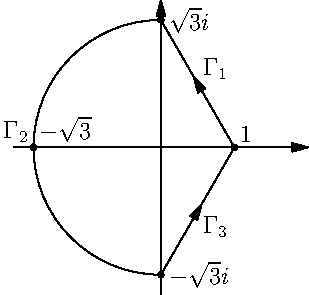
\includegraphics{Gamma_pre}
    \caption{The shape of $\Gamma^{\pre}$. It differs from $\Gamma$ only locally around $1$.}
    \label{fig:Gamma_pre}
  \end{minipage}
  \hfill
  \begin{minipage}[t]{0.45\linewidth}
    \centering
    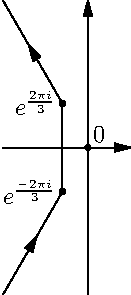
\includegraphics{tilde_Gamma}
    \caption{The shapes of $\tilde{\Gamma}$ and $\tilde{\Gamma}^{\infty}$ around $0$. For $\tilde{\Gamma}^{\infty}$ the contour extents to infinity, and for $\tilde{\Gamma}$ it extends to $N^{1/30} e^{\pm 2\pi i/3}$. $\tilde{\Gamma}$ has the same shape as $\Gamma \cap N_{\delta_N}(1)$ up to scaling.}
    \label{fig:tilde_Gamma}
  \end{minipage}
\end{figure}
We show that $\Re h(z)$ attains its global maximum on $\Gamma^{\pre}$ at $1$  by explicit computation. For $z \in \Gamma_1$, we write $z = (1 - t) + i\sqrt{3}t$ where $t \in [0, 1]$. Then
\begin{equation}
  \Re h(z) = 2(1 - t) - \frac{1}{2}(1 - 2t - 2t^2) - \log \sqrt{(1 - t)^2 + 3t^2} - 1
\end{equation}
and for $t \in (0, 1)$
\begin{equation}
  \frac{d}{dt} \Re h(z) = \frac{8t^3 - 8t^2}{1 - 2t + 4t^2} = \frac{8t^2 (t - 1)}{(1 - t)^2 + 3t^2} < 0.
\end{equation}
Hence $\Re h(z)$ decreases as $z$ moves from $1$ to $\sqrt{3}i$ along $\Gamma_1$. Since $\Gamma_2$ is symmetric to $\Gamma_1$ about the real axis and $h(z)$ is a real analytic function, $\Re h(z)$ decreases as $z$ moves from $1$ to $-i\sqrt{3}$ along $\Gamma_2$. For $z \in \Gamma_3$, denote $z = \sqrt{3}(\cos\theta + i\sin\theta)$ where $\theta \in [\pi/2, 3\pi/2]$. Then for $z \in \Gamma_3$
\begin{equation}
  \begin{split}
    \Re h(z) = {}& \frac{1}{2} - 3\cos^2\theta + 2\sqrt{3}\cos\theta - \log \sqrt{3} \\
    = {}& \frac{1}{2} + 1 - (1 - \sqrt{3}\cos\theta)^2 - \log \sqrt{3} \\
    \leq {}& \frac{1}{2} - \log \sqrt{3} < \Re h(1).
  \end{split}
\end{equation}
Thus $\Gamma^{\pre}$ satisfies the requirement of the steepest-descent contour in Step \ref{enu:steepest_descent_method_contour}. $\Gamma$ is defined by deforming $\Gamma^{\pre}$ such that the two points $1 + N^{-1/3}e^{\pm 2\pi i/3}$ are joint by a vertical line segment instead of a polygonal chain through $1$. See Figure \ref{fig:tilde_Gamma} for this local part of $\Gamma$ maginified.

By Taylor expansion around $1$,
\begin{equation}
  h(z) = h(1) + \frac{1}{6} h'''(1) (z - 1)^3 + \bigO((z - 1)^4) = \frac{1}{2} - \frac{(z - 1)^3}{3} + \bigO((z - 1)^4).
\end{equation}
Consider $\delta_N = N^{-3/10}$. The two points $1 + \delta_N e^{\pm 2\pi i/3}$ are on $\Gamma$, and
\begin{equation}
  h(1 + \delta_N e^{\pm 2\pi i/3}) = \frac{1}{2} - \frac{1}{3} N^{-\frac{9}{10}} + \bigO(N^{-\frac{6}{5}})
\end{equation}
and then
\begin{equation}
  \Re h(1 + \delta_N e^{\pm 2\pi i/3}) < \frac{1}{2} - \epsilon N^{-\frac{9}{10}}
\end{equation}
for an $\epsilon > 0$. From the construction of $\Gamma$, we can verify that
\begin{equation}
  \Re h(z) < \frac{1}{2} - \epsilon N^{-\frac{9}{10}}
\end{equation}
for all $z \in \Gamma \setminus N_{\delta_N}(1)$. Hence
\begin{equation} \label{eq:noness_part_steepest_descent}
  \begin{split}
    & \left\lvert \frac{1}{2\pi i} \oint_{\Gamma \setminus N_{\delta_N(1)}} e^{Nh(z)} g(z) dz \right\rvert \\
    \leq {}& \left\lvert \frac{1}{2\pi i} \oint_{\Gamma \setminus N_{\delta_N(1)}} e^{N(\frac{1}{2} - \epsilon N^{-\frac{9}{10}})} \lvert g(z) \rvert \lvert dz \rvert \right\rvert \\
    = {}& e^{- \epsilon N^{-\frac{9}{10}}} e^{\frac{1}{2} N} \left\lvert \frac{1}{2\pi i} \oint_{\Gamma \setminus N_{\delta_N(1)}} e^{N(\frac{1}{2} - \epsilon N^{-\frac{9}{10}})} \lvert g(z) \rvert \lvert dz \rvert \right\rvert = C e^{- \epsilon N^{-\frac{9}{10}}} e^{\frac{1}{2} N} \\
  \end{split}
\end{equation}
where $C$ depends on the behavior of $g(z)$ on $\Gamma$.

On the other hand, on $\Gamma \cap N_{\delta_N}(1)$, we take the change of variable $z = 1 + N^{-1/3}w$ and have
\begin{equation} \label{eq:exp(h)_when_x=2}
  e^{N h(z)} = e^{N(\frac{1}{2} - \frac{1}{3}(z - 1)^3 + \bigO((z - 1)^4))} = e^{\frac{N}{2}} e^{-\frac{w^3}{3}} e^{\bigO(N^{-\frac{1}{5}})} = e^{\frac{N}{2}} e^{-\frac{w^3}{3}} (1 + \bigO(N^{-\frac{1}{5}})),
\end{equation}
where we use the estimate that for $z \in N_{\delta_N}(1)$, $(z - 1)^4 = \bigO(N^{-6/5})$. Thus
\begin{equation} \label{eq:ess_part_steepest_descent}
  \begin{split}
    \frac{1}{2\pi i} \oint_{\Gamma \cap N_{\delta_N(1)}} e^{Nh(z)} g(z) dz = {}& N^{-\frac{1}{3}} \frac{1}{2\pi i} \oint_{\tilde{\Gamma}} e^{\frac{N}{2}} e^{-\frac{w^3}{3}} (1 + \bigO(N^{-\frac{1}{5}})) dw \\
    = {}& N^{-\frac{1}{3}}  e^{\frac{N}{2}} (1 + \bigO(N^{-\frac{1}{5}})) \frac{1}{2\pi i} \oint_{\tilde{\Gamma}^{\infty}} e^{-\frac{w^3}{3}} dw \\
    = {}& N^{-\frac{1}{3}}  e^{\frac{N}{2}} (1 + \bigO(N^{-\frac{1}{5}})) \Ai(0).
  \end{split}
\end{equation}
Here the contours $\tilde{\Gamma}$ and $\tilde{\Gamma}^{\infty}$ are described in Figure \ref{fig:tilde_Gamma}, and we use the Airy function to denote the integral in \eqref{eq:ess_part_steepest_descent}. The Airy function is a special function with many applications. See \cite{Abramowitz-Stegun64} for its various properties. The general formula of the Airy function is, in its contour integral formula,
\begin{equation} \label{eq:Airy_func}
  \Ai(x) = \frac{1}{2\pi i} \oint_{\tilde{\Gamma}^{\infty}}
  e^{-\frac{w^3}{3} + xw} dw.
\end{equation}
It is easy to see that the integrand in \eqref{eq:Airy_func}, although defined on an infinite contour, converges for all $x \in \compC$.

Now we consider more generally $x = 2 + N^{-2/3 \xi}$ where $\xi$ is in a compact subset of $\compC$. Although we are interested mostly in real value of $x$, it is harmless and actualy useful to consider complex $x$. Then
\begin{equation}
  h(z) = 2z - \frac{z^2}{2} - \log z - 1 + N^{-\frac{2}{3}} \xi z - N^{-\frac{2}{3}} \xi - \frac{1}{4} N^{-\frac{4}{3}} \xi^2,
\end{equation}
and for $z \in N_{\delta_N}(1)$, after the change of variable $z = 1 + N^{-1/3}w$, we have like \eqref{eq:exp(h)_when_x=2}
\begin{equation}
  e^{N h(z)} = e^{\frac{N}{2}} e^{-\frac{w^3}{3} + \xi w} (1 + \bigO(N^{-\frac{1}{5}})).
\end{equation}
Thus like \eqref{eq:ess_part_steepest_descent}
\begin{equation} \label{ess_part_steepest_descent_generalized}
  \begin{split}
    \frac{1}{2\pi i} \oint_{\Gamma \cap N_{\delta_N(1)}} e^{Nh(z)} g(z) dz = {}& N^{-\frac{1}{3}}  e^{\frac{N}{2}} (1 + \bigO(N^{-\frac{1}{5}})) \frac{1}{2\pi i} \oint_{\tilde{\Gamma}^{\infty}} e^{-\frac{w^3}{3} + \xi w} g(1) dw \\
    = {}& N^{-\frac{1}{3}} g(1) e^{\frac{N}{2}} (1 + \bigO(N^{-\frac{1}{5}})) \Ai(\xi).
  \end{split}
\end{equation}
On the other hand, since the ingegrand is only slightly changed, the estimate of the integral over $\Gamma \setminus N_{\delta_N}(1)$, which is not as sensitive as the integral near the critical point, barely changes, and we still have like \eqref{eq:noness_part_steepest_descent}
\begin{equation} \label{eq:noness_part_steepest_descent_generalized}
  \left\lvert \frac{1}{2\pi i} \oint_{\Gamma \setminus N_{\delta_N(1)}} e^{Nh(z)} g(z) dz \right\rvert < C e^{- \epsilon N^{-\frac{9}{10}}} e^{\frac{N}{2}}.
\end{equation}
The detail is left to the reader. 

The asymptotics \eqref{ess_part_steepest_descent_generalized} and the estimate \eqref{eq:noness_part_steepest_descent_generalized}, together with the asymptotics \eqref{eq:asy_of_C_N}, imply that as $N \to \infty$, for $x = 2 + N^{-2/3}\xi$ and $\xi$ is in a compact subset of $\realR$,
\begin{equation} \label{eq:asy_of_p_N}
  p_N(x) e^{-\frac{N}{4}x^2} = N^{\frac{1}{6}} (1 + \bigO(N^{-\frac{1}{5}}) \Ai(\xi).
\end{equation}

As $x \to +\infty$, the Airy function $\Ai(x) \to 0$ exponentially. Actually
\begin{equation}
  \Ai(x) = \frac{e^{-\frac{2}{3} x^{\frac{3}{2}}}}{2 \sqrt{\pi} x^{\frac{1}{4}}}, \quad \text{as $x \to +\infty$}.
\end{equation}
It suggests that the asymptotic formula for $p_N(x) e^{-Nx^2/4}$ can be extrapolated so show that it vanishes exponentially as $x$ increases. However, we need always to be cautious to do extrapolation. Below we give an expenential decay result, which is not the optimal one, but suffices for our purpose.

We distinguish $h(z)$ with different parameters $x$, and write
\begin{equation}
  h_{\xi}(z) = \left. h(z) \right\rvert_{x = 2 + N^{-\frac{2}{3} \xi}} = 2z - \frac{z^2}{2} - \log z + N^{-\frac{2}{3}} \xi z - 1 - N^{-\frac{2}{3}} \xi - \frac{1}{4} N^{-\frac{4}{3}} \xi^2.
\end{equation}
Then we have for all $\xi \in \realR_+$ and all $z \in \Gamma$
\begin{equation}
  \Re(h_{\xi}(z) - h_0(z)) = N^{-\frac{2}{3}} \xi \left( \Re z - 1 - \frac{1}{4} N^{-\frac{2}{3}} \xi \right) < -N^{-1} \frac{\xi}{2},
\end{equation}
where we use that $\Re z \leq 1 - N^{-1/3}/2$ for all $z \in \Gamma$. Thus
\begin{equation} \label{eq:ratio_h_xi_h_0}
  \lvert e^{N h_{\xi}(z)} \rvert < e^{-\frac{\xi}{2}} \lvert e^{N h_0(z)} \rvert
\end{equation}
for all $z \in \Gamma$.

Recall the computation of $p_N(x) e^{-Nx^2/4}$ for $x = 2$, especially \eqref{eq:noness_part_steepest_descent} and \eqref{eq:ess_part_steepest_descent}. We see that we can use almost the same computation to derive that
\begin{equation}
  \int_{\Gamma} \lvert e^{N h_0(z)} \rvert \lvert g(z) \rvert \lvert dz \rvert < C N^{-\frac{1}{3}} e^{\frac{N}{2}},
\end{equation}
where $C = \bigO(1)$ is a positive constant. Hence \eqref{eq:contour_int_p_N_N-1} and \eqref{eq:ratio_h_xi_h_0} imply
\begin{equation}
  \left. p_N(x) e^{-\frac{N}{4}x^2} \right\rvert_{x = 2 + N^{-\frac{2}{3} \xi}} < \frac{1}{2\pi} \int_{\Gamma} \lvert e^{N h_{\xi}(z)} \rvert \lvert g(z) \rvert \lvert dz \rvert = \frac{C_N}{2\pi} e^{-\frac{\xi}{2}} C N^{-\frac{1}{3}} e^{\frac{N}{2}} = e^{-\frac{\xi}{2}} \frac{C}{2\pi} N^{-\frac{1}{6}} (1 + \bigO(N^{-1})),
\end{equation}
where the $\bigO(N^{-1})$ term comes from the Stirling formula of $C_N$ and is independent of $\xi$. We conclude that as $x = 2 + N^{-\frac{2}{3} \xi}$ and $\xi > 0$, $p_N(x) e^{-Nx^2/4}$ decays exponentially with respect to $\xi$. A slight stretch of the computation shows that the exponential decay holds if $\xi$ is complex, with its imaginary part bounded.

Now we have asymptotics of $p_N(x) e^{-Nx^2/4}$. The method can be applied to $p_{N - 1}(x) e^{-Nx^2/4}$ verbatim, since the only difference between their contour integral formulas is from the $g(z)$ factor, but all our derivation does not use any specific property of $g(z)$. Similar to \eqref{eq:asy_of_p_N}, we have that for $x = 2 + N^{-2/3}\xi$ and $\xi$ is in a compact subset of $\compC$
\begin{equation} \label{eq:asy_of_p_N-1}
  p_{N - 1}(x) e^{-\frac{N}{4}x^2} = N^{\frac{1}{6}} (1 + \bigO(N^{-\frac{1}{5}}) \Ai(\xi),
\end{equation}
and we also have the exponential decay property as $\xi \to +\infty$. However, if we substitute formulas \eqref{eq:asy_of_p_N} and \eqref{eq:asy_of_p_N-1} into \eqref{eq:GUE_maximum}, we get no meaningful result.

The situation can be saved in a simple way. Write
\begin{equation} \label{eq:alternative_K_N}
    K_N(x, y) = \frac{(p_N(x) - p_{N - 1}(x))e^{-\frac{N}{4}x^2} p_{N - 1}(y)e^{-\frac{N}{4}y^2} - p_{N - 1}(x)e^{-\frac{N}{4}x^2} (p_N(y) - p_{N - 1}(y))e^{-\frac{N}{4}y^2}}{x - y},
\end{equation}
and express
\begin{equation}
  (p_N(x) - p_{N - 1}(x))e^{-\frac{N}{4}x^2} = \frac{C_N}{2\pi i} \oint_{\Gamma} e^{N h(z)} g(z) dz,
\end{equation}
where
\begin{equation}
  h(z) = xz - \frac{z^2}{2} - \log z - \frac{x^2}{4}, \quad g(z) = z^{-1} - 1.
\end{equation}
The estimation of the integral over $\Gamma \setminus N_{\delta_N}(1)$ can be done similarly to \eqref{eq:noness_part_steepest_descent}, and the same result can be obtained. But since the saddle point $1$ is a zero of $g(z)$, the integral over $\Gamma \cap N_{\delta_N(1)}$ need to be modified a little. With the change of variable $z = 1 + N^{-1/3}w$, we have similar to \eqref{eq:ess_part_steepest_descent} and \eqref{ess_part_steepest_descent_generalized}
\begin{equation}
  \begin{split}
    \frac{1}{2\pi i} \oint_{\Gamma \cap N_{\delta_N(1)}} e^{Nh(z)} g(z) dz = {}& N^{-\frac{1}{3}} \frac{1}{2\pi i} \oint_{\tilde{\Gamma}} e^{\frac{N}{2}} e^{-\frac{w^3}{3} + \xi w} (-N^{-\frac{1}{3}}w) (1 + \bigO(N^{-\frac{1}{5}})) dw \\
    = {}& -N^{-\frac{2}{3}}  e^{\frac{N}{2}} (1 + \bigO(N^{-\frac{1}{5}})) \frac{1}{2\pi i} \oint_{\tilde{\Gamma}^{\infty}} e^{-\frac{w^3}{3} + \xi w} w dw \\
    = {}& -N^{-\frac{2}{3}}  e^{\frac{N}{2}} (1 + \bigO(N^{-\frac{1}{5}})) \frac{d}{d\xi} \left( \frac{1}{2\pi i} \oint_{\tilde{\Gamma}^{\infty}} e^{-\frac{w^3}{3} + \xi w} dw \right) \\
    = {}& -N^{-\frac{2}{3}}  e^{\frac{N}{2}} (1 + \bigO(N^{-\frac{1}{5}})) \Ai'(\xi),
  \end{split}
\end{equation}
and then
\begin{equation} \label{eq:asy_of_p_N-p_N-1}
  (p_N(x) - p_{N - 1}(x))e^{-\frac{N}{4}x^2} = -N^{-\frac{1}{6}}  (1 + \bigO(N^{-\frac{1}{5}})) \Ai'(\xi).
\end{equation}
Furthermore we know that it decays exponentially with respect to $\xi$ as $\xi \to +\infty$.

We define the kernel function
\begin{equation}
  K_{\Airy}(\xi, \eta) =
  \begin{cases}
    {\displaystyle \frac{\Ai(\xi)\Ai'(\eta) - \Ai'(\xi)\Ai(\eta)}{\xi - \eta}} & \text{if $\xi \neq \eta$,} \\
    \Ai'(\eta)^2 - \Ai''(\eta)\Ai(\eta) & \text{if $\xi = \eta$.}
  \end{cases}
\end{equation}
Note that $K(\xi, \eta)$ is analytic in both $\xi$ and $\eta$. The asymptotics \eqref{eq:asy_of_p_N}, \eqref{eq:asy_of_p_N-1}, \eqref{eq:asy_of_p_N-p_N-1} and the identity \eqref{eq:alternative_K_N} immdiately give as that as $x = 2 + N^{-2/3}\xi$ and $y = 2 + N^{-2/3}\eta$, where $\xi, \eta$ are in a compact subset of $\realR$ and $\xi \neq \eta$,
\begin{equation}
  \lim_{N \to \infty} N^{-\frac{2}{3}} K_N(x, y) = K_{\Airy}(\xi, \eta).
\end{equation}
By a little complex analysis, we can generalise it to the $\xi = \eta$ case. For any $\eta$, we consider
\begin{equation}
  \xi_{\theta} = \eta + e^{i\theta}, \quad \text{and} \quad x_{\theta} = 2 + \xi_{\theta}.
\end{equation}
Then the Cauchy integral formula implies that
\begin{equation}
  \lim_{N \to \infty} N^{-\frac{2}{3}} K_N(y, y) = \lim_{N \to \infty} \int^{2\pi}_0 N^{-\frac{2}{3}} K_N(x_{\theta}, y) d\theta = \frac{1}{2\pi} \int^{2\pi}_0 K_{\Airy}(\xi_{\theta}, \eta) d\theta = K_{\Airy}(\eta, \eta).
\end{equation}

Now we have the pointwise convergence that $N^{-2/3}K_N(x, y) \to K_{\Airy}(\xi, \eta)$. We also know that as $\xi, \eta \to \pm \infty$, $\lvert N^{-2/3}K_N(x, y) \rvert$ vanishes uniformly. Then by argument in functional analysis, we have that if $a = 2 + N^{-2/3} T$, then
\begin{equation}
  \lim_{N \to \infty} \det( 1 - \id_{(a, \infty)}(x) K_N(x, y) \id_{(a, \infty)}(y)) = F_{\TW}(T) := \det(1 - \id_{(T, \infty)}(\xi) K_{\Airy}(\xi, \eta) \id_{(T, \infty)}(\eta)).
\end{equation}
Here the $F_{\TW}$ is the cumulative distribution function of the celebrated Tracy-Widom distribution. Finally we have the result for the limiting distribution of the largest eigenvalue in GUE:
\begin{thm}
  As the dimension $N \to \infty$, the largest eigenvalue $\lambda_{\max}$ in GUE is almost surely at $2$, and its fluctuation is of order $N^{-2/3}$, given by the Tracy-Widom distribution that
  \begin{equation}
    \lim_{N \to \infty} \Prob(\lambda_{\max} < 2 + N^{-2/3}T) = F_{\TW}(T).
  \end{equation}
\end{thm}
We are not going to give the proof of this theorem, unless we have enough time left in the end of this semester.

\paragraph{Exercise}

\begin{enumerate}
\item 
  Complete the proof of Lemma \ref{lem:very_good_Lebesgue} for the $k = 3, \dotsc, N$ case. (Hint: Cauchy-Binet formula is an important linear algebraic identity that you can learn from \url{http://en.wikipedia.org/wiki/Cauchy–Binet_formula}, for example.
\item
  The \emph{Laguerre polynomials} (see \cite{Szego75} and \url{http://en.wikipedia.org/wiki/Laguerre_polynomials})
  \begin{equation}
    L^{(\alpha)}_n(x) = \frac{1}{2\pi i} \oint \frac{e^{\frac{xt}{1 - t}}}{(1 - t)^{\alpha + 1} t^{n + 1}} dt
  \end{equation}
  where $\alpha > -1$ is a parameter, and the contour encloses $0$ but not $1$.

  Find an asymptotic formula involving Airy function of $e^{-x/2} L^{(0)}_n(x)$ for $x = 4n + 2 + 2(2n/3)^{1/3} t$ where $n \to \infty$ and $t$ is in a compact subset of $\realR$.
\end{enumerate}

\section{Limiting distribution of the largest eigenvalue in Gaussian $\beta$ ensemble}

We have derived the Tracy-Widom distribution for the limiting distribution of the largest eigenvalue in the GUE random matrices. For Gaussian orthogonal ensemble (GOE) and Gaussian symplectic ensemble (GSE), similar results hold, but the derivation becomes more sophisticated. Although the limiting distribution of the largest eigenvalues is a problem in probability, the solution for GUE as shown in Section \ref{sec:local_prop_GUE} and these for GOE and GSE rely on the exploit of the symmetry of the models and analytical techniques not commonly seen in probability literature. For people inclining to study probability, we present a unified solution for the limiting distribution of the largest eigenvalue in GUE, GOE and GSE. The drawback of this approach is that the result is stated in a rather abstract way.

This section follows closely to \cite[Section 4.5]{Anderson-Guionnet-Zeitouni10}. Another good reference is the Ph.D.\@ \href{https://tspace.library.utoronto.ca/bitstream/1807/31693/3/Bloemendal_Alex_201111_PhD_Thesis.pdf}{thesis} of Alex Bloemendal \cite{Bloemendal11}. The interested readers are refered to the original paper by \Ramirez, Rider and \Virag\ \cite{Ramirez-Rider-Virag11} that contains more results about the $\beta$ ensembles.

\begin{rmk}
  In this section, the terms ``Gaussian unitary ensemble'' and ``Gaussian orthogonal ensemble'' are defined slightly different from those in Section \ref{sec:semicircle_law}. For GUE, we define it as a random Hermitian matrix such that the diagonal entries are real and in $\Normal(0, 1)$, upper-triangular entries are complex with both real and imaginary parts in independent $\Normal(0, \frac{1}{2})$ distributions, and they are all independent. So it is the GUE in Section \ref{sec:semicircle_law} scaled up by $N$. The GOE (as well as GSE) is redefined by the same scaling.
\end{rmk}

\subsection{Tridiagonal matrix models and the Gaussian $\beta$ ensemble}

We are going to define a tridiagonal random matrix model that has a parameter $\beta > 0$, such that the distribution of the eigenvalues in the tridiagonal random matrix model with $\beta = 1, 2, 4$ is identical to that of the eigenvalues in GOE, GUE and GSE respectively. Thus we call this tridiagonal random matrix model \emph{Gaussian $\beta$ ensemble} (G$\beta$E). The limiting distributions of the largest eigenvalue in GOE, GUE and GSE become those of the largest eigenvalue in the G$\beta$E for the corresponding $\beta$.

First we recall the $\chi_t$ distribution that is a positive continuous probability distribution given by the density function
\begin{equation}
  f_t(x) = \frac{2^{1 - \frac{t}{2}} x^{t - 1} e^{-\frac{x^2}{2}}}{\Gamma(\frac{t}{2})} \id_{(0, \infty)}(x),
\end{equation}
where the real parameter $t > 0$. When $t$ is an integer, $\chi_t$ distribution is related to the normal distribution in the way that if $X_1, \dotsc, X_t$ are \iid\ random variables in distribution $\Normal(0, 1)$, then
\begin{equation} \label{eq:chi_and_normal}
  \left( \sum^t_{i = 1} X^2_i \right)^{\frac{1}{2}} \sim \chi_t(x).
\end{equation}
If $t$ is an integer, then it is a direct consequence of \eqref{eq:chi_and_normal} and the central limit theorem that as $t \to \infty$
\begin{equation} \label{eq:CLT_chi}
  2(\chi_t(x) - \sqrt{t}) \todistr \Normal(0, 1).
\end{equation}
A straightforward computation confirms that \eqref{eq:CLT_chi} holds for real $t$.

We define the Gaussian $\beta$ ensemble as follows. Let $\xi_1, \xi_2, \dotsc, Y_1, Y_2, \dotsc$ be independent random variables such that $\xi_i \sim N(0, 1)$ and $Y_i \sim \xi_{i\beta}$. For any dimension $N$, the $N$ dimensional symmetric matrix $H_N$ in G$\beta$E is given by
\begin{align}
  h_{ij} = {}& 0 \quad \text{if} \quad \lvert i - j \rvert > 1, \\
  h_{ii} = {}& \sqrt{2/\beta} \xi_i, \label{eq:defn_h_ii} \\
  h_{i, i + 1} = {}& h_{i + 1, i} = Y_{N - i}/\sqrt{\beta}. \label{eq:defn_h_ii+1} 
\end{align}
Then we have
\begin{thm} \label{thm:Edelman_Dumitriu}
  For any $\beta$ and $N$, let $\lambda_1, \dotsc, \lambda_N$ be the eigenvalues of $H_N$. Then the joint probability density function of $\lambda_1, \dotsc, \lambda_N$ is
  \begin{equation}
    P_{\beta}(\lambda_1, \dotsc, \lambda_N) = \frac{1}{C_{N, \beta}} \Delta(\lambda)^{\beta} e^{-\frac{\beta}{4} \sum^N_{i = 1} \lambda^2_i}.
  \end{equation}
\end{thm}
When $\beta = 2$, Theorem \ref{thm:Edelman_Dumitriu} shows that the G$\beta$E has the same spectral property as GUE. In Exercise \ref{enu:ex_4_1} we will see that the G$\beta$E with $\beta = 1$ has the same spectral property as GOE. The relation between G$\beta$E with $\beta = 4$ and GSE is analogous, but the proof is a little too complicated to be an exercise.

\begin{proof}[Proof of Theorem \ref{thm:Edelman_Dumitriu} for $\beta = 2$]
  First we show the eqivalence between the distribution of eigenvalues of G$\beta$E with $\beta = 2$ and GUE, and prove the theorem for $\beta = 2$. For any $N$, let the $N \times N$ random Hermitian matrix $X_N = (x_{ij})^N_{i, j = 1}$ be a GUE random matrix, such that
  \begin{equation}
    X_N =
    \begin{pmatrix}
      \Normal(0, 1) & \Normal(0, \frac{1}{2}) + i \Normal(0, \frac{1}{2}) & \dots & \Normal(0, \frac{1}{2}) + i \Normal(0, \frac{1}{2}) \\
      \Normal(0, \frac{1}{2}) + i \Normal(0, \frac{1}{2}) & \Normal(0, 1) & \dots & \Normal(0, \frac{1}{2}) + i \Normal(0, \frac{1}{2}) \\
      \vdots & \vdots & & \vdots \\
      \Normal(0, \frac{1}{2}) + i \Normal(0, \frac{1}{2}) & \Normal(0, \frac{1}{2}) + i \Normal(0, \frac{1}{2}) & \dots & \Normal(0, 1)
    \end{pmatrix}
  \end{equation}
  where all the upper diagonal entries are independent. Since any unitary similarity transformation does not change the spectrum of a matrix, we define a random unitary operator $U(1) \in \Unitary(N - 1)$ that depends on $X_N$ such that
  \begin{enumerate}
  \item
    Let $\vec{x}_1 = (x_{21}, x_{31}, \dotsc, x_{N1})^T$. Then
    \begin{equation}
      U(1) \vec{x}_1 = \lVert \vec{x}_1 \rVert \vec{e}_1 = (\lVert \vec{x}_1 \rVert, 0, \dotsc, 0)^T.
    \end{equation}
  \item
    $U(1) \vec{x} = \vec{x}$ if $\vec{x}$ is orthogonal to $\vec{x}_1$ and $\vec{e}_1$.
  \end{enumerate}
  This unitary transformation is the \emph{Householder transformation} \cite[Section 2.2.4]{Horn-Johnson90}
  \begin{equation}
    U(1) = I - 2\frac{\vec{u}\vec{u}^*}{\lVert \vec{u} \rVert^2}, \quad \text{where} \quad \vec{u} = \vec{x}_1 - \lVert \vec{x}_1 \rVert \vec{e}_1.
  \end{equation}
  Then we define the unitary matrix $\tilde{U}(1) \in \Unitary(N)$ by
  \begin{equation}
    \tilde{U}(1) = I_{1 \times 1} \oplus U(1), \quad \text{or equivalently} \quad \tilde{U}(1) =
    \begin{pmatrix}
      1 & 0 \\
      0 & U(1)
    \end{pmatrix}.
  \end{equation}
  Then
  \begin{equation}
    \tilde{U}(1) X_N \tilde{U}(1)^{-1} =
    \begin{pmatrix}
      x_{11} & \lVert \vec{x}_1 \rVert & 0 & \dots & 0 \\
      \lVert \vec{x}_1 \rVert & & & & \\
      0 & & & & \\
      \vdots & & X_{N - 1} & & \\
      0 & & & &
    \end{pmatrix},
  \end{equation}
  where $X_{N - 1}$ is a random matrix defined as
  \begin{equation}
    X_{N - 1} = U(1) (X_N)_{11} U(1)^{-1},
  \end{equation}
  where $(X_N)_{11}$ is the $(N - 1)$ dimensional matrix obtained by removing the first row and first column of $X_N$.

  Note that $x_{11} \sim \Normal(0, 1)$ and
  \begin{equation}
    \lVert \vec{x}_1 \rVert = \left( \sum^N_{i = 2} (\Re x_{i2})^2 + (\Im x_{i2})^2 \right)^{\frac{1}{2}} \sim \frac{1}{\sqrt{2}} \chi_{2(N - 1)}
  \end{equation}
  since both $\Re x_{ij}$ and $\Im x_{ij}$ are in $\Normal(0, \frac{1}{2})$ distribution for $i \neq j$. Thus $\tilde{U}(1) X_N \tilde{U}(1)^{-1}$ agrees with the tridiagonal matrix $H_N$ in the first column and the first row.

  $(X_N)_{11}$ is a random Hermitian matrix different from the $(N - 1)$ dimensional GUE only by scaling. Thus by Exercise \ref{enu:Ex_Sec_1:1} in Section \ref{sec:three_Gaussian_ensembles}, its distribution is invariant under unitary similarity transformation. Note that the result in the exercise is valid when the unitary similarity transformation is fixed. Here $U(1)$ is random, but by its construction, $U(1)$ depends only on entries of $X_N$ that are not in $(X_N)_{11}$, so $U(1)$ is independent of $(X_N)_{11}$, and then the result of the exercise still holds. Also we have that $X_{N - 1}$ is independent of $U(1)$, and if we write $X_{N - 1} = (\tilde{x}_{ij})^{N - 1}_{i, j = 1}$, all $\tilde{x}_{ij}$ are independent of $x_{11}$ and $\lVert \vec{x}_1 \rVert$.

  Let $U(2) \in \Unitary(N - 2)$ be a Householder transformation sending $\vec{x}_2 = (\tilde{x}_{21}, \tilde{x}_{31}, \dotsc, \tilde{x}_{N - 1, 1})^T$ into $\lVert \vec{x}_2 \rVert \vec{e}_1$ and keeping vectors orthogonal to $\vec{x}_2$ and $\vec{e}_1$ invariant. Then denoting $\tilde{U}(2) = I_{2 \times 2} \oplus U(2)$, we have
    \begin{equation}
      \tilde{U}(2) \tilde{U}(1) X_N \tilde{U}(1)^{-1} \tilde{U}(2)^{-1} =
    \begin{pmatrix}
      x_{11} & \lVert \vec{x}_1 \rVert & 0 & 0 & \dots & 0 \\
      \lVert \vec{x}_1 \rVert & \tilde{x}_{11} & \lVert \vec{x}_2 \rVert & 0 & & 0 \\
      0 & \lVert \vec{x}_2 \rVert & & & & \\
      0 & 0 & & & & \\
      \vdots & \vdots & & X_{N - 2} & & \\
      0 & 0 & & & &
    \end{pmatrix},
  \end{equation}
  which agrees with $H_N$ in the first two columns and the first two rows, where $X_{N - 2}$ is defined analogously to $X_{N - 1}$. Repeat the construction $N - 1$ times, we have finally that $ \tilde{U}(N - 1) \dotsm \tilde{U}(2) \tilde{U}(1) X_N \tilde{U}(1)^{-1} \tilde{U}(2)^{-1} \dotsm \tilde{U}(N - 1)^{-1}$ is the tridiagonal random matrix $H_N$ that has the same spectral property as $X_N$.
\end{proof}

Now we prove the general case. Denote the $N \times N$ tridiagonal matrix
\begin{equation} \label{eq:J_N}
  J_N =
  \begin{pmatrix}
    a_0 & b_1 & & & \\
    b_1 & a_1 & b_2 & & \\
     & b_2 & \ddots & \ddots & \\
     & & \ddots & a_{N - 2} & b_{N - 1} \\
     & & & b_{N - 1} & a_{N - 1}
  \end{pmatrix}.
\end{equation}
Without loss of generality, we assume that $b_1, \dotsc, b_{N - 1}$ are all strictly positive. Suppose $\lambda_1 \geq \dotsb \geq \lambda_N$ are eigenvalues of $J_N$ and $\vec{v}_1, \dotsc, \vec{v}_N$ are corresponding eigenvectors. Note that if $\lambda_i$'s are distinct, then $\vec{v}_i$'s are fixed up to a scalar multiple.
\begin{lem} \label{lem:distinct_eigenvalue_H_N}
  The eigenvalues $\lambda_1, \dots, \lambda_N$ are distinct. Furthermore, writing $\vec{v}_i = (v_i(1), \dotsc, v_i(N))^T$, we have $v_i(1) \neq 0$.
\end{lem}
\begin{proof}
  The identity $J_N  \vec{v}_i = \lambda_i \vec{v}_i$ is expressed as
  \begin{equation}
    \begin{pmatrix}
      a_0 - \lambda_i & b_1 & & & \\
      b_1 & a_1 - \lambda_i & b_2 & & \\
       & b_2 & \ddots & \ddots & \\
       & & \ddots & a_{N - 2} - \lambda_i & b_{N - 1} \\
       & & & b_{N - 1} & a_{N - 1} - \lambda_i 
    \end{pmatrix}
    \begin{pmatrix}
      v_i(1) \\
      v_i(2) \\
      \vdots \\
      v_i(N - 1) \\
      v_i(N)
    \end{pmatrix}
    = \vec{0},
  \end{equation}
  or componentwise
  \begin{equation} \label{eq:iterative_equations_of_v_i(n)}
    \left\{
      \begin{aligned}
        (a_0 - \lambda_i) v_i(1) + b_1 v_i(2) = {}& 0, \\
        b_1 v_i(1) + (a_1 - \lambda_i) v_i(2) + b_2 v_i(3) = {}& 0, \\
        \vdots & \\
        b_{N - 2} v_i(N - 2) + (a_{N - 2} - \lambda_i) v_i(N - 1) + b_{N - 1} v_i(N) = {}& 0, \\
        b_{N - 1} v_i(N - 1) + (a_{N - 1} - \lambda_i) v_i(N) = {}& 0.
      \end{aligned}
    \right.
  \end{equation}
  If $v_i(1) = 0$, then iteratively we find all components to be zero, and then the vector is a zero vector. For any nonzero $v_i(1)$, iteratively we can uniquely solve $v_i(2), \dotsc, v_i(N)$ by the first, \dots, $(N - 1)$-th equations in \eqref{eq:iterative_equations_of_v_i(n)}. Then the eigenspace associated to $\lambda_i$ is $1$-dimensional, and $\lambda_1, \dotsc, \lambda_N$ are distinct.
\end{proof}
Converse to Lemma \ref{lem:distinct_eigenvalue_H_N}, we have
\begin{lem} \label{lem:distinct_eigenvalue_H_N_reverse}
  Given a diagonal matrix
  \begin{equation} \label{eq:diagonal_related_to_H_N}
    D = \diag(\lambda_1, \dots \lambda_N) \quad \text{where} \quad \lambda_1 > \dotsb > \lambda_N.
  \end{equation}
  and a unit row vector $\vec{u} = (u_1, \dotsc, u_N)$ such that all its components are strictly positive and $\sum^N_{i = 1} u^2_i = 1$, there exists a tridiagonal matrix $J_N$ expressed as in \eqref{eq:J_N} such that $b_1, \dotsc, b_{N - 1}$ are strictly positive, and
  \begin{equation}
    J_N = O D O^{-1}
  \end{equation}
  where $O = (o_{ij})^N_{i, j = 1} \in \Orthogonal(N)$ with the first row $o_{1j} = u_j$. 
\end{lem}
\begin{proof}
  We relate tridiagonal matrices with orthogonal polynomials. Given a measure $\mu$ on $\realR$, let $p_0(x), p_1(x), \dotsc$ be orthogonal polynomials of degree $0, 1, \dotsc$ such that
  \begin{equation} \label{eq:ortho_poly_again}
    \int p_i(x) p_j(x) d\mu(x) = \delta_{ij}.
  \end{equation}
  Then the three term-recurrence formula is (assuming $a_{-1} = 0$)
  \begin{equation} \label{eq:3_term_recur}
    x p_n(x) = b_n p_{n + 1}(x) + a_n p_n(x) + b_{n - 1} p_{n - 1}(x),
  \end{equation}
  or equivalently (note that the $a_i, b_i$ in \eqref{eq:3_term_recur} and \eqref{eq:3_term_recur_matrix} are not consistent with those in \eqref{eq:J_N})
  \begin{equation} \label{eq:3_term_recur_matrix}
    x
    \begin{pmatrix}
      p_0(x) \\
      p_1(x) \\
      \vdots \\
      \vdots
    \end{pmatrix}
    =
    \begin{pmatrix}
      a_0 & b_1 & & \\
      b_1 & a_1 & b_2 & \\
      & b_2 & \ddots & \ddots \\
      & & \ddots & 
    \end{pmatrix}
    \begin{pmatrix}
      p_0(x) \\
      p_1(x) \\
      \vdots \\
      \vdots
    \end{pmatrix}.
  \end{equation}
  Truncate the $N \times N$ upper left block of the operator on the right-hand side of \eqref{eq:3_term_recur_matrix}, we get a tridiagonal matrix. Note that $b_i > 0$ if we choose all the orthogonal polynomials $p_i(x)$ to have positive leading coefficient.
  
  Suppose $\mu$ is a measure on $\realR$ supported on $N$ points $\lambda_1, \dotsc, \lambda_N$, such that
  \begin{equation}
    \mu(x) = \sum^N_{i = 1} c_i \delta_{\lambda_i}(x),
  \end{equation}
  where we assume $c_i \neq 0$. Then the space $L^2(\mu)$ is an $N$ dimensional space. Obviously $L^2(\mu)$ is spanned by $\{\id_{\lambda_1}(x), \dotsc, \id_{\lambda_N}(x) \}$, and it is also spanned by $\{ 1, x, \dotsc, x^{N - 1} \}$ by the Lagrange interpolation formula. Given that the orthogonal polynomials $p_0(x), \dotsc, p_{N - 1}(x)$ exist, (the existence of the orthogonal polynomials can be proved and is left as an exercise), then $\{ p_0(x), \dotsc, p_{N - 1}(x) \}$ is also a basis.

  Furthermore, the basis
  \begin{equation}
    B_1 = \{ \frac{1}{c_i} \id_{\lambda_i}(x) \overset{\text{a.e.\ in $\mu$}}{=} \frac{1}{c_i} \prod_{k = 1, \dotsc, N, k \neq i} \frac{x - \lambda_k}{\lambda_i - \lambda_k} \mid i = 1, \dotsc, N \}
  \end{equation}
  is an orthonormal basis of $L^2(\mu)$ for which the multiplication operator $x$ has the matrix representation $D$ in \eqref{eq:diagonal_related_to_H_N}, while the basis
  \begin{equation}
    B_2 = \{ p_{i - 1}(x) \mid i = 1, \dotsc, N \}
  \end{equation}
  is another orthogonal basis of $L^2(\mu)$ for which the multiplication operator $x$ has the matrix representation $J_N$ in \eqref{eq:J_N}.

  The identity $J_N = O D O^{-1}$ means that
  \begin{equation}
    \begin{pmatrix}
      p_0(x) \\
      \vdots \\
      p_{N - 1}(x)
    \end{pmatrix}
    = O
    \begin{pmatrix}
      c^{-1}_1 \id_{\lambda_1}(x) \\
      \vdots \\
      c^{-1}_N \id_{\lambda_N}(x)
    \end{pmatrix},
  \end{equation}
  and especially
  \begin{equation}
    \left( \sum^N_{i = 1} c^2_i \right)^{-\frac{1}{2}} = p_0(x) \overset{\text{a.e.\ in $\mu$}}{=} o_{11} \frac{1}{c_1} \id_{\lambda_1}(x) + \dotsb + o_{1N} \frac{1}{c_N} \id_{\lambda_N}(x).
  \end{equation}
  This identity is satisfied when $c_i = o_{1i}$. Thus we conclude that the matrix constructed from the three-term recurrence relation for the orthogonal polynomials $p_i(x)$ defined by \eqref{eq:ortho_poly_again} with $\mu$ given by 
  \begin{equation}
    \mu(x) = \sum^N_{i = 1} u_i \delta_{\lambda_i}(x),
  \end{equation}
  and the property that $b_i > 0$ are satisfied if we require all $p_i(x)$ to have positive leading coefficients.
\end{proof}

Lemmas \ref{lem:distinct_eigenvalue_H_N} and \ref{lem:distinct_eigenvalue_H_N_reverse} define a bijection between the space of tridiagonal matrices $H_N$ with strictly positive $b_i$ as denoted in \eqref{eq:J_N} and the space of $(D, \vec{u})$ where the diagonal matrix $D$ and the unit vector $\vec{u}$ satisfy the conditions in Lemma \ref{lem:distinct_eigenvalue_H_N_reverse}. We denote this map from $H_N$ to $(D, \vec{u})$ as
\begin{equation}
  F: \Delta_N \times S^{N - 1}_+ \to \realR^N \times (0, \infty)^{N - 1},
\end{equation}
where
\begin{align}
  \Delta_N = {}& \{ (x_1, \dotsc, x_N) \in \realR^N \mid x_1 > \dotsb > x_N \}, \\
  S^{N + 1}_+ = {}& \{(x_1, \dotsc, x_{N - 1}) \in (0, \infty)^{N - 1} \mid 0 < \sum^{N - 1}_{i = 1} x^2_i < 1 \},
\end{align}
and
\begin{equation}
  F(\lambda_1, \dotsc, \lambda_N; u_1, \dotsc, u_{N - 1}) = (a_0, \dotsc, a_{N - 1}; b_1, \dotsc, b_{N - 1}).
\end{equation}
Obviously $F$ is differentiable, and we have
\begin{lem} \label{lem:beta_Jacobian}
  The Jacobian of $F$ is
  \begin{equation} \label{eq:beta_Jacobian}
    \frac{\partial(a_0, \dotsc, a_{N - 1}; b_1, \dotsc, b_{N - 1})}{\partial(\lambda_1, \dotsc, \lambda_N; u_1, \dotsc, u_{N - 1})} = C \frac{\Delta(\lambda)}{\prod^{N - 1}_{i = 1} b^{N - j - 1}_j}.
  \end{equation}
\end{lem}
The proof of Lemma \ref{lem:beta_Jacobian} relies on the following technical result
\begin{lem}
  Any element in the set of $N \times N$ Hermitian matrices, except for those in a subset of Lebesgue measure $0$ (or equivalently, probability $0$ in GUE), can be written uniquely as
  \begin{equation} \label{eq:decompose_real_ortho}
    X = O^{-1} D O,
  \end{equation}
  where $D = \diag(\lambda_1, \dotsc, \lambda_N)$ and $\lambda_1 < \lambda_2 < \dotsb < \lambda_N$, and $O = (o_{ij})^N_{i, j = 1} \in \Orthogonal(N)$ such that $o_{11}, o_{21}, \dotsc, o_{N1}$ are all strictly positive.
\end{lem}
We are not going to prove this lemma, since its proof is parallel to those of Lemmas \ref{lem:repeated_eigenvalues}, \ref{lem:nonzero_U} and \ref{eq:unitary_parametrized} in Section \ref{subsec:jpdf_GUE}.
\begin{proof}[Proof of Lemma \ref{lem:beta_Jacobian}]
  By Exercise \ref{enu:ex_4_1}, we have that given an $N \times N$ random real symmetric matrix $X_N$ in GOE (as defined in this section), by the tridiagonalisation procedure we get a random tridiagonal matrix whose distribution is exactly the same as $H_N$ with $\beta = 1$. The tridiagonal procedure is (analogous to the proof of Theorem \ref{thm:Edelman_Dumitriu} for $\beta = 2$)
  \begin{equation}
    X_N \to \tilde{O}(N - 1) \dotsm \tilde{O}(2) \tilde{O}(1) X_N \tilde{O}(1)^{-1} \tilde{O}(2)^{-1} \dotsm \tilde{O}(N - 1)^{-1},
  \end{equation}
  where
  \begin{equation}
    \tilde{O}(k) =
    \begin{pmatrix}
      I_k & 0 \\
      0 & O(k)
    \end{pmatrix}
    \quad \text{and} \quad O(k) \in \Orthogonal(N - k).
  \end{equation}
  Suppose $X_N$ has the unique decomposition \eqref{eq:decompose_real_ortho}, then the tridiagonalisation procedure becomes
  \begin{equation}
    O^{-1} D O \to \tilde{O}^{-1} D \tilde{O}, \quad \text{where} \quad \tilde{O} = (\tilde{o}_{ij})^N_{i, j = 1} = O \tilde{O}(1)^{-1} \dotsm \tilde{O}(N - 1)^{-1}.
  \end{equation}
  We observe that the first column of $\tilde{O}$ is identical to that of $O$. Therefore by Lemma \ref{lem:distinct_eigenvalue_H_N_reverse}, we conclude that the tridiagonalisation procedure transforms real symmetric matrices $X_N$ (except for those in a measure $0$ subset) whose unique decomposition \eqref{eq:decompose_real_ortho} has eigenvalues $\lambda_1, \dotsc, \lambda_N$ and first column of $O$ as $o_{i1} = u_1$ ($i = 1, \dotsc, N$) to the tridiagonal matrix $J_N$ denoted in \eqref{eq:J_N} such that
  \begin{equation}
    a_0, \dotsc, a_{N - 1}; b_1, \dotsc, b_{N - 1} = F(\lambda_1, \dotsc, \lambda_N; u_1, \dotsc, u_{N - 1}).
  \end{equation}

  Suppose we have the marginal distribution of $\lambda_1, \dotsc, \lambda_N; u_1, \dotsc, u_{N - 1}$, then by the bijectivity results in Lemmas \ref{lem:distinct_eigenvalue_H_N} and \ref{lem:distinct_eigenvalue_H_N_reverse}, the distribution of $a_0, \dotsc, a_{N - 1}; b_1, \dotsc, b_{N - 1}$ is
  \begin{equation} \label{eq:relation_of_marginal_pdf}
    P(a_0, \dotsc, a_{N - 1}; b_1, \dotsc, b_{N - 1}) = P(\lambda_1, \dotsc, \lambda_N; u_1, \dotsc, u_{N - 1}) \frac{\partial(a_0, \dotsc, a_{N - 1}; b_1, \dotsc, b_{N - 1})}{\partial(\lambda_1, \dotsc, \lambda_N; u_1, \dotsc, u_{N - 1})}.
  \end{equation}

  We take a special choice of $X_N$ such that $X_N$ is in the GOE distribution. Then we have the marginal distribution
  \begin{equation} \label{eq:marginal_pdf_lambda_u}
    P(\lambda_1, \dotsc, \lambda_N; u_1, \dotsc, u_{N - 1}) = \frac{1}{C} \Delta(\lambda) \prod^N_{i = 1} e^{\frac{1}{4}jj \lambda^2_i},
  \end{equation}
  where $C$ does not depend on $\lambda_i$ or $u_i$. (The proof is similar to the arguments in Section \ref{subsec:jpdf_GUE}, and we are not going to give any detail. On the other hand, we have by Exercise \ref{enu:ex_4_1} that 
  \begin{equation} \label{eq:pdf_tridiagonal_beta=1}
    P(a_0, \dotsc, a_{N - 1}; b_1, \dotsc, b_{N - 1}) = \frac{1}{C} \prod^{N - 1}_{i = 0} e^{-\frac{1}{4} a^2_i} \prod^{N - 1}_{j = 1} e^{-\frac{1}{2} b^2_j} b^{N - j - 1}_j.
  \end{equation}
  Noting that
  \begin{equation}
    \prod^{N - 1}_{i = 0} e^{-\frac{1}{4} a^2_i} \prod^{N - 1}_{j = 1} e^{-\frac{1}{2} b^2_j} = e^{-\frac{1}{4} \Tr(J^2_N)} = \prod^N_{i = 1} e^{-\frac{1}{4} \lambda^2_i},
  \end{equation}
  we derive \eqref{eq:beta_Jacobian} from \eqref{eq:relation_of_marginal_pdf}, \eqref{eq:marginal_pdf_lambda_u} and \eqref{eq:pdf_tridiagonal_beta=1}.
\end{proof}

For the proof of Theorem \ref{thm:Edelman_Dumitriu}, we need another technical result
\begin{lem} \label{lem:beta_Jacobian_next}
  With notations the same as in Lemma \ref{lem:beta_Jacobian}, we have
  \begin{equation} \label{eq:beta_Jacobian_next}
    \prod^{N - 1}_{j = 1} b^{N - j}_j = \Delta(\lambda) \prod^N_{i = 1} u_i.
  \end{equation}
\end{lem}
\begin{proof}
  Let $\vec{e}_1 = (1, 0, 0, \dotsc, 0)^T$. We have
  \begin{align}
    J_N \vec{e}_1 = {}& (a_0, b_1, 0, \dotsc, 0), \\
    J^2_N \vec{e}_1 = {}& (a^2_0 + b_1 b_0, a_0 b_1 + b_1 a_1, b_1 b_2, \dotsc, 0), \\
    \vdots {}& \notag
  \end{align}
  Then
  \begin{equation}
    \det(\vec{e}_1, J_N \vec{e}_1, J^2_N \vec{e}_1, \dotsc, J^{N - 1}_N \vec{e}_1) =
    \begin{pmatrix}
      1 & * & * & \dots & * \\
      0 & b_1 & * & \dots & * \\
      0 & 0 & b_1 b_2 & & * \\
      \vdots & \vdots & \vdots & \ddots & \vdots \\
      0 & 0 & 0 & \dots & b_1 b_2 \dotsm b_{N - 1}
    \end{pmatrix}
    = \prod^{N - 1}_{j = 1} b^{N - j}_j.
  \end{equation}
  On the other hand, using the decomposition $J_N = O^{-1} D O$ where $D = \diag(\lambda_1, \dotsc, \lambda_N)$ and $\lambda_i$ are increasing, and the first column of $O$ is given by $\vec{u} = (u_1, \dotsc, u_N)^T$, we have
  \begin{equation}
    \begin{split}
      \det(\vec{e}_1, J_N \vec{e}_1, J^2_N \vec{e}_1, \dotsc, J^{N - 1}_N \vec{e}_1) = {}& \det(O^{-1} D^0 O \vec{e}_1, O^{-1} D^1 O \vec{e}_1, \dotsc, O^{-1} D^{N - 1} O \vec{e}_1) \\
      = {}& \det(O^{-1}(D^0 O \vec{e}_1, D^1 O \vec{e}_1, \dotsc, D^{N - 1} O \vec{e}_1)) \\
      = {}& \det(O^{-1}) \det(D^0 \vec{u}, D^1 \vec{u}, \dotsc, D^{N - 1} \vec{u})) \\
      = {}& \pm
      \begin{vmatrix}
        u_1 & \lambda_1 u_1 & \dots & \lambda^{N - 1}_1 u_1 \\
        u_1 & \lambda_2 u_1 & \dots & \lambda^{N - 1}_2 u_1 \\
        \vdots & \vdots & \dots & \vdots \\
        u_1 & \lambda_N u_1 & \dots & \lambda^{N - 1}_N u_1
      \end{vmatrix} \\
      = {}& \pm \Delta(\lambda) \prod^N_{i = 1} u_i.
    \end{split}
  \end{equation}
  The sign ambiguity can be solved since $\Delta(\lambda)$ is positive. Then we prove \eqref{eq:beta_Jacobian_next}.
\end{proof}
\begin{proof}[Proof of Theorem \ref{thm:Edelman_Dumitriu} for $\beta > 0$]
  The results in Lemmas \ref{lem:beta_Jacobian} and \ref{lem:beta_Jacobian_next} together imply that
  \begin{equation}
    \frac{\partial(a_0, \dotsc, a_{N - 1}; b_1, \dotsc, b_{N - 1})}{\partial(\lambda_1, \dotsc, \lambda_N; u_1, \dotsc, u_{N - 1})} = \frac{\prod^{N - 1}_{j = 1} b_j}{\prod^N_{i = 1} u_i}.
  \end{equation}
  For the $N$ dimensional random tridiagonal matrix $H_N$ defined in the beginning of this subsection, in probability $1$ the entries of $h_{i, i + 1} = h_{i + 1, i}$ are strictly positive, so we identify it with $J_N$ in \eqref{eq:J_N} and use $a_0, \dotsc, a_{N - 1}; b_1, \dotsc, b_{N - 1}$ to denote its nontrivial entries. From the distribution of $a_0, \dotsc, a_{N - 1}; b_1, \dotsc, b_{N - 1}$ and the Jacobian \eqref{eq:beta_Jacobian}, we compute the joint probability density of $\lambda_1, \dotsc, \lambda_N; u_1, \dotsc, u_{N - 1}$ as
  \begin{equation}
    \begin{split}
      P(\lambda_1, \dotsc, \lambda_N; u_1, \dotsc, u_{N - 1}) = {}& P(a_0, \dotsc, a_{N - 1}; b_1, \dotsc, b_{N - 1}) \frac{\partial(a_0, \dotsc, a_{N - 1}; b_1, \dotsc, b_{N - 1})}{\partial(\lambda_1, \dotsc, \lambda_N; u_1, \dotsc, u_{N - 1})} \\
      = {}& C \prod^{N - 1}_{i = 0} e^{-\frac{\beta}{4} a^2_i} \prod^{N - 1}_{j = 1} b^{\beta(N - j) - 1}_j e^{-\frac{\beta}{2} b^2_j} \frac{\prod^{N - 1}_{j = 1} b_j}{\prod^N_{i = 1} u_i} \\
      = {}& C e^{-\frac{\beta}{4} \Tr H^2_N} \frac{\prod^{N - 1}_{j = 1} b^{\beta(N - j)}_j}{\prod^N_{i = 1} u_i} \\
      = {}& C \Delta(\lambda)^{\beta} \prod^N_{i = 1} e^{-\frac{\beta}{4} \lambda^2_i} \left( \prod^N_{i = 1} u_i \right)^{\beta - 1}.
    \end{split}
  \end{equation}
  Integrating out $u_1, \dotsc, u_{N - 1}$, we obtain the distribution of $\lambda_1, \dotsc, \lambda_N$ as in Theorem \ref{thm:Edelman_Dumitriu}.
\end{proof}

\subsection{Limiting distribution of the largest eigenvalue in Gaussian $\beta$ ensemble}

Before the statement of the result on the limiting distribution of the largest eigenvalue of $H_N$, we give a heuristic argument to motivate the theorem and its proof. From our result for the largest eigenvalue in GUE that is equivalent to the special case of $H_N$ with $\beta = 2$, we conjecture that the largest eigenvalue is around $2\sqrt{N}$ with fluctuation $\bigO(N^{-1/6})$. Write
\begin{equation}
  \begin{split}
    \tilde{H}_N = {}& N^{\frac{1}{6}} (H_N - 2\sqrt{N}I) \\
    = {}&
    \begin{pmatrix}
      -2N^{\frac{2}{3}} + \sqrt{\frac{2}{\beta}} N^{\frac{1}{6}} \xi_1 & \frac{1}{\sqrt{\beta}} N^{\frac{1}{6}} Y_{N - 1} & & \\
      \frac{1}{\sqrt{\beta}} N^{\frac{1}{6}} Y_{N - 1} & -2N^{\frac{2}{3}} + \sqrt{\frac{2}{\beta}} N^{\frac{1}{6}} \xi_2 & \frac{1}{\sqrt{\beta}} N^{\frac{1}{6}} Y_{N - 2} & \\
      & \frac{1}{\sqrt{\beta}} N^{\frac{1}{6}} Y_{N - 2} & -2N^{\frac{2}{3}} + \sqrt{\frac{2}{\beta}} N^{\frac{1}{6}} \xi_3 & \ddots \\
      & & \ddots & \ddots 
    \end{pmatrix} \\
    = {}&
    \begin{pmatrix}
      -2N^{\frac{2}{3}} + \sqrt{\frac{2}{\beta}} N^{\frac{1}{6}} \xi_1 & N^{\frac{1}{6}} \sqrt{N - 1} + \frac{1}{\sqrt{2\beta}} N^{\frac{1}{6}} \xi'_1 & & \\
      N^{\frac{1}{6}} \sqrt{N - 1} + \frac{1}{\sqrt{2\beta}} N^{\frac{1}{6}} \xi'_1 & -2N^{\frac{2}{3}} + \sqrt{\frac{2}{\beta}} N^{\frac{1}{6}} \xi_2 & N^{\frac{1}{6}} \sqrt{N - 2} + \frac{1}{\sqrt{2\beta}} N^{\frac{1}{6}} \xi'_2 & \\
       & N^{\frac{1}{6}} \sqrt{N - 2} + \frac{1}{\sqrt{2\beta}} N^{\frac{1}{6}} \xi'_2 & -2N^{\frac{2}{3}} + \sqrt{\frac{2}{\beta}} N^{\frac{1}{6}} \xi_3 & \ddots \\
       & & \ddots & \ddots
    \end{pmatrix},
  \end{split}
\end{equation}
where $\xi'_i = \sqrt{2}(Y_{N - i} - \sqrt{(N - i)\beta})$, and from \eqref{eq:CLT_chi} we have that the distribution of $\xi'_i$ is close to $\Normal(0, 1)$ if $i$ is not close to $N$.

The matrix $\tilde{H}_N$ acts on $N$-dimensional vector $(f_1, f_2, \dotsc, f_N)^T$. Define a function $f(x)$ on $[0, N^{2/3}]$ such that
\begin{equation} \label{eq:equiv_vector_step_func}
  f(x) = f_i \quad \text{for} \quad x \in [(i - 1)N^{-\frac{1}{3}}, iN^{-\frac{1}{3}}).
\end{equation}
The function $f(x)$ is not continuous, let alone differentiable. But we assume that $f(x)$ is a ``discretised'' continuous, or even smooth, function with step length $N^{-1/3}$. One way to think of it is to let $\tilde{f}(x)$ be a smooth function, and $f(x) = \tilde{f}((i - 1)N^{-1/3})$ where $i$ is the smallest possible number such that $i N^{-1/3} \geq x$. Then heuristically (as commonly used in numerical analysis of smooth functions)
\begin{align}
  f_{i + 1} - f_i \approx {}& N^{-\frac{1}{3}} f'(i N^{-\frac{1}{3}}), \\
  f_{i + 1} - 2f_i + f_{i - 1} \approx {}& N^{-\frac{1}{3}} f'(i N^{-\frac{1}{3}}) - N^{-\frac{1}{3}} f'((i - 1) N^{-\frac{1}{3}}) \approx N^{-\frac{2}{3}} f''(i N^{-\frac{1}{3}}).
\end{align}

For $i = x N^{1/3}$ where $x \in (0, \infty)$, the vector identity
\begin{equation}
  \begin{split}
    \tilde{H}_N
    \begin{pmatrix}
      \vdots \\
      f_i \\
      \vdots
    \end{pmatrix}
    = {}&
    \begin{pmatrix}
      \vdots \\
      \begin{gathered}
        (N^{\frac{1}{6}} \sqrt{N - i + 1} + \frac{N^{\frac{1}{6}}}{\sqrt{2\beta}} \xi'_{i - 1}) f_{i - 1} + (-2N^{\frac{2}{3}} + \sqrt{\frac{2}{\beta}} N^{\frac{1}{6}} \xi_i) f_i \\
        + (N^{\frac{1}{6}} \sqrt{N - i} + \frac{N^{\frac{1}{6}}}{\sqrt{2\beta}} \xi'_i) f_{i + 1}
      \end{gathered} \\
      \vdots
    \end{pmatrix} \\
    = {}&
    \begin{pmatrix}
      \vdots \\
      \begin{gathered}
        N^{\frac{2}{3}} (f_{i - 1} + f_i + f_{i + 1}) + (N^{\frac{1}{6}} \sqrt{N - i + 1} - N^{\frac{2}{3}}) f_{i - 1} + (N^{\frac{1}{6}} \sqrt{N - i} - N^{\frac{2}{3}}) f_{i + 1} \\
        + N^{\frac{1}{6}} \left( \frac{1}{\sqrt{2\beta}} \xi'_{i - 1} f_{i - 1} + \sqrt{\frac{2}{\beta}} \xi_i f_i + \frac{1}{\sqrt{2\beta}} \xi'_i f_{i + 1} \right) 
      \end{gathered} \\
      \vdots
    \end{pmatrix}
  \end{split}
\end{equation}
can be approximated, by the identities
\begin{equation}
  N^{\frac{1}{6}} \sqrt{N - i + 1} - N^{\frac{2}{3}} \approx -\frac{x}{2}, \quad N^{\frac{1}{6}} \sqrt{N - i} - N^{\frac{2}{3}} \approx -\frac{x}{2}
\end{equation}
and $f_{i - 1} \approx f_i \approx f_{i + 1}$, as
\begin{equation} \label{eq:approx_of_tilde_H_N}
  \tilde{H}(f)(x) \approx f''(x) - x f(x) + \frac{2}{\sqrt{\beta}} N^{\frac{1}{6}} \left(\frac{1}{2\sqrt{2}} \xi'_{i - 1} + \frac{1}{\sqrt{2}} \xi_i + \frac{1}{2\sqrt{2}} \xi'_{i + 1} \right) f(x).
\end{equation}
Note that as $N \to \infty$,
\begin{equation}
  \frac{1}{2\sqrt{2}} \xi'_{i - 1} + \frac{1}{\sqrt{2}} \xi_i + \frac{1}{2\sqrt{2}} \xi'_{i + 1} \todistr \Normal(0, 1).
\end{equation}
We relate this factor in normal distribution to Brownian motion $B_x$. It is well known that $B_x$ is not differentiable. But if we consider the discretised derivative of $B_x$ with step length $N^{-1/3}$, we have
\begin{equation}
  \frac{B_{x + N^{-\frac{1}{3}}} - B_x}{N^{-\frac{1}{3}}} \sim N^{\frac{1}{6}} \Normal(0, 1).
\end{equation}
Thus we can write \eqref{eq:approx_of_tilde_H_N} as
\begin{equation}
  H_N(f)(x) \approx \Hbeta(f)(x),
\end{equation}
where the stochastic differential operator
\begin{equation}
  \Hbeta = \frac{d^2}{d x^2} - x + B'_x.
\end{equation}
\begin{rmk}
  When we approximate $N^{1/6} (\frac{1}{2\sqrt{2}} \xi'_{i - 1} + \frac{1}{\sqrt{2}} \xi_i + \frac{1}{2\sqrt{2}} \xi'_{i + 1})$ by $B'_x$, we violate the martingale property of $B_x$, that is, $B'_x$ and $B'_{x + N^{-1/3}}$ should be independent. To solve this discrepency, we aproximate $N^{1/6} \xi_i$ by $B_x(1)'$ and approximate $N^{1/6} \xi_i$ by $B_x(2)'$ where $B_x(1)$ and $B_x(2)$ are independent Brownian motions. Then $N^{1/6} (\frac{1}{2\sqrt{2}} \xi'_{i - 1} + \frac{1}{\sqrt{2}} \xi_i + \frac{1}{2\sqrt{2}} \xi'_{i + 1})$ is approximated by $\frac{1}{2\sqrt{2}} B_{x - N^{-1/3}}(2)' + \frac{1}{\sqrt{2}} B_x(1)' + \frac{1}{2\sqrt{2}} B_x(2)'$, and this is in some sense close to a Brownian motion.
\end{rmk}

The next question is, how to make sense of the stochastic differential operator (that is sometimes called \emph{Stochastic Airy operator}). The $B'_x$ term does not make sense, but it makes sense in distribution: If $h(x)$ is a function such that it has compact support and $h'(x)$ exists and is continuous, then for any continuous but not necessarily differentiable function $f$, we can talk about its derivative in the sense that
\begin{equation}
  \int f'(x) h(x) dx = - \int f(x) h'(x) dx.
\end{equation}
We use this idea, together with that the path of $B_x$ is continuous, to rigorously define $\Hbeta$.

For any $f, g \in C^{\infty}_0(0, \infty)$, \ie, smooth functions of compact support in $(0, \infty)$, we define the inner product
\begin{equation}
  \langle f, g \rangle_* = \int^{\infty}_0 f'(x) g'(x) dx + \int^{\infty}_0 (1 + x) f(x) g(x) dx,
\end{equation}
and then define $\Lstar$  as the Hilbert space that is the completion of $C^{\infty}_0(0, \infty)$ with respect to the inner product $\langle \cdot, \cdot \rangle_*$, and denote $\lVert f \rVert_* = \langle f, f \rangle_*$ for the norm of $f \in\Lstar$. Readers familiar with Sobolev spaces can see immediately the similarity between our $\Lstar$ and $H^1_0(0, \infty)$, which is defined as the Hilbert space obtained as the completion of smooth functions of compact support in $(0, \infty)$ with respect to the inner product
\begin{equation}
  \langle f, g \rangle_{H^1(0, \infty)} = \int^{\infty}_0 f'(x) g'(x) dx + \int^{\infty}_0 f(x) g(x) dx.
\end{equation}
The norm $\lVert f \rVert_{H^1(0, \infty)}$ is also defined similar to $\lVert f \rVert_*$. Below we give some basic properties of the space $\Lstar$.

\begin{lem} \label{lem:various_convergences}
  The point set of $\Lstar$ can be realised as a subset of \Holder\ $\frac{1}{2}$-continuous functions on $(0, \infty)$. Then for any $f \in \Lstar \in C^{0, \frac{1}{2}}(0, \infty)$, we have $f(0) := \lim_{x \to 0^*} f(x) = 0$ and for all $x > 1$
  \begin{equation} \label{eq:thm:Lstar}
    (x + 1)^{\frac{1}{4}} \lvert f(x) \rvert \leq \sqrt{2} \lVert f \rVert_*.
  \end{equation}
\end{lem}
\begin{proof}
  Comparing $\langle \cdot, \cdot \rangle_*$ with $\langle \cdot, \cdot \rangle_{H^1(0, \infty)}$, we see that any $f \in \Lstar$ satisfies $\lVert f \rVert_{H^1(0, \infty)} \leq \lVert f \rVert_*$ and then $\Lstar$ can be embedded into $H^1_0(0, \infty)$ naturally. It is a standard result that $H^1_0(0, \infty)$ can be embedded into $C^{0, \frac{1}{2}}(0, \infty)$ \cite[Theorem 4.12, Part II]{Adams-Fournier03}. Hence we have the embedding result from $\Lstar$ to the space of \Holder\ $\frac{1}{2}$-continuous functions. Furthermore, the Sobolev embedding theorem also imply that on any finite closed interval $I = [a, b] \in [0, \infty)$, there is a constant $C$ depending on $b - a$ only such that
  \begin{multline} \label{eq:Holder_norm}
    \lVert f \rVert_{C^{0, \frac{1}{2}}(I)} := \max_{x \in I}(\lvert f(x) \rvert) + \max_{x_1, x_2 \in I} \frac{f(x_1) - f(x_2)}{\sqrt{\lvert x_1 - x_2 \rvert}} \\
    < C \left( \int^b_a f(x)^2 + f'(x)^2 dx \right)^{\frac{1}{2}} \leq C \lVert f \rVert_{H^1_0(0, \infty)} \leq \lVert f \rVert_*.
  \end{multline}
  Let $f \in \Lstar \subset C^{0, \frac{1}{2}}(0, \infty)$ and $f = \lim_{n \to \infty} f_n$ where $f_n \in C^{\infty}_0(0, \infty)$. Since $f_n(0) = 0$, we have $f(0) = 0$ by the convergence in \Holder\ norm \eqref{eq:Holder_norm}. Below we prove the inequality \eqref{eq:thm:Lstar}. By the convergence in \Holder\ norm, we only need to consider $f \in C^{\infty}_0(0, \infty)$.  To prove \eqref{eq:thm:Lstar}, We show that for $f \in C^{\infty}_0(0, \infty)$,
  \begin{equation} \label{eq:intermediate_ineq}
    f(x)^2 \leq 4 \lVert f \rVert_{L^2(x, \infty)} \lVert f' \rVert_{L^2(x, \infty)}, \quad \text{where} \quad \lVert \phi \rVert_{L^2(x, \infty)} = \left( \int^{\infty}_x \phi(t)^2 dt \right)^{\frac{1}{2}} \quad \text{for $\phi = f, f'$}.
  \end{equation}
  Suppose \eqref{eq:intermediate_ineq} does not hold for $f$, without loss of generality we assume that there is $x > 0$ such that $f(x) > 0$ and $f(x)^2 > 4\lVert f \rVert_{L^2(x, \infty)} \lVert f' \rVert_{L^2(x, \infty)}$. Then in the set $A_x = \{ y: 0 < y - x < \frac{1}{4} f(x)^2 / \lVert f' \rVert^2_{L^2(x, \infty)} \}$, because
  \begin{equation}
    \lvert f(y) - f(x) \rvert = \left\lvert \int^y_x f'(t) dt \right\rvert < \left( \int^y_x f'(t)^2 dt \right)^{\frac{1}{2}} \sqrt{y-x} \leq \lVert f' \rVert_{L^2(x, \infty)},
  \end{equation}
  we have
  \begin{equation}
    f(y) \geq f(x) - \sqrt{\lvert y - x \rvert} \lVert f' \rVert_{L^2(x, \infty)} \geq f(x) - \frac{1}{2} \frac{f(x)}{\lVert f' \rVert_{L^2(x, \infty)}} \lVert f' \rVert_{L^2(x, \infty)} = \frac{1}{2} f(x),
  \end{equation}
  and get the contradiction that
  \begin{equation}
    \lVert f \rVert^2_{L^2(x, \infty)} \geq \int_{A_x} f(t)^2 dt > \left( \frac{1}{2} f(x) \right)^2 \cdot \frac{1}{4} \frac{f(x)^2}{\lVert f' \rVert^2_{L^2(x, \infty)}} > \lVert f \rVert^2_{L^2(x, \infty)}.
  \end{equation}
  Then we prove \eqref{eq:thm:Lstar} by combining \eqref{eq:intermediate_ineq} with the inequality
  \begin{equation}
    \begin{split}
      \lVert f \rVert^2_* \geq {}& \int^{\infty}_x (1 + t) f(t)^2 dt + \int^{\infty}_x f'(t)^2 dt \\
      \geq {}& (x + 1) \lVert f \rVert^2_{L^2(x, \infty)} + \lVert f' \rVert^2_{L^2(x, \infty)} \\
      \geq {}& 2\sqrt{x + 1} \lVert f \rVert_{L^2(x, \infty)} \lVert f' \rVert_{L^2(x, \infty)}.
    \end{split}
  \end{equation}
\end{proof}
Due to the embedding property of $\Lstar$ into $C^{0, \frac{1}{2}}[0, \infty)$, we assume all elements of $\Lstar$ as continuous functions.
\begin{lem}
  Let $\{ f_n \}$ be a bounded sequence in $\Lstar$, then we can choose a subsequence $\{ f_{n_k} \} \subseteq \{ f_n \}$ and a $f \in \Lstar$ and have
  \begin{enumerate}
  \item \label{enu:thm:Lstar_L^2}
    $L^2$ convergence: $f_{n_k} \to f$ in $L^2(0, \infty)$.
  \item  \label{enu:thm:Lstar_weak1}
    Weak $L^2$ convergence in derivative: $f'_{n_k} \to f'$ weakly in $L^2(0, \infty)$, that is, for any $h \in L^2(0, \infty)$, $\langle f'_{n_k}, h \rangle_2 \to \langle f', h \rangle_2$.
  \item \label{enu:thm:Lstar_local_uniform}
    Locally uniform convergence: On any compact subset of $(0, \infty)$, $f_{n_k} \to f$ uniformly.
  \item \label{enu:thm:Lstar_weak2}
    Weak $\Lstar$ convergence: $f_{n_k} \to f$ weakly in $\Lstar$, that is, for any $h \in \Lstar$, $\langle f_{n_k}, h \rangle_* \to \langle f, h \rangle_*$.
  \end{enumerate}
\end{lem}
\begin{proof}
  Property \ref{enu:thm:Lstar_weak2} is direct consequence of the Banach-Alaoglu theorem. Noting that the boundedness of $\lVert f \rVert_*$ implies the boundedness of $\lVert f' \rVert_2$, we find property \ref{enu:thm:Lstar_weak1} to be the sequence of the Banach-Alaoglu theorem as well. By the inequality \eqref{eq:Holder_norm}, the boundedness in $\Lstar$ norm implies the uniform boundedness and equicontinuous over a compact interval, so property \ref{enu:thm:Lstar_local_uniform} is proved by the \Arzela-Ascoli theorem. Property \ref{enu:thm:Lstar_local_uniform} immediately implies that given any $C > 0$, a subsequence $\{ f_{n_k} \}$ converges in $L^2(0, C)$ if we consider these functions on $(0, C)$. The condition that $\int^{\infty}_0 (1 + x) f_n(x)^2 dx \leq \lVert f \rVert^2_*$ is bounded implies that the result holds when $C = \infty$. The detail is left as an exercise.
\end{proof}

We call a pair $(f, \lambda) \in \Lstar \times \realR$ an \emph{eigenvector-eigenvalue pair} of $\Hbeta$, if $\lVert f \rVert_2 := \lVert f \rVert_{L^2(0, \infty)} = 1$ and $\Hbeta f = \lambda f$ in the sense of Schwarz distribution, \ie, for any test  function $\phi(x) \in C^{\infty}_0(0, \infty)$,
\begin{equation} \label{eq:defining_prop_pair:1}
  \lambda \int^{\infty}_0 f(x) \phi(x) dx = \int^{\infty}_0 \left[ f''(x) - xf(x) + \frac{2}{\sqrt{\beta}} B'_x f(x) \right] \phi(x) dx,
\end{equation}
or equivalently
\begin{equation} \label{eq:defining_prop_pair:2}
  \lambda \int^{\infty}_0 f(x) \phi(x) dx = \int^{\infty}_0 f(x) \left[ \phi''(x) - x \phi(x) - \frac{2}{\sqrt{\beta}} B_x \phi'(x) \right] - \frac{2}{\sqrt{\beta}} f'(x) B_x \phi(x) dx.
\end{equation}

Now we can state the main result in this section
\begin{thm} \label{thm:RRV}
  Fix $\beta > 0$. Let $\lambda^N_N \geq \lambda^N_{N - 1} \geq \dotsb$ be eigenvalues of $H_N$. We consider any $k \in \intZ_+$.
  \begin{enumerate}
  \item \label{enu:thm:RRV:1}
    For almost any Brownian motion path $B_x$, $\Hbeta$ has well defined largest, second largest, \dots, $k$-th largest eigenvalues $\lambda_1, \dotsc, \lambda_k$ and all of them are simple eigenvalues.
  \item \label{enu:thm:RRV:2}
    The random vector $N^{1/6}(\lambda^N_N - 2\sqrt{N}, \dotsc, \lambda^N_{N - k + 1} - 2\sqrt{N})$ converges in distribution to $(\lambda_1, \dotsc, \lambda_k)$ as $N \to \infty$.
  \end{enumerate}
\end{thm}

To prove part \ref{enu:thm:RRV:1} of Theorem \ref{thm:RRV}, we introduce a bilinear form on $\Lstar$ associated with $\Hbeta$. Suppose $f, g \in C^{\infty}_0(0, \infty) \subset \Lstar$ are smooth functions, we inteprete $\Hbeta g$ as a distribution, and define
\begin{equation}
  \begin{split}
    \langle f, g \rangle_{\Hbeta} = {}& -\int^{\infty}_0 (\Hbeta g)(x) f(x) dx \\
    = {}& -\int^{\infty}_0 f(x) \left( g''(x) - xg(x) + \frac{2}{\sqrt{\beta}} B'_x g(x) \right) dx \\
    = {}& \int^{\infty}_0 f'(x) g'(x) dx + \int^{\infty}_0 xf(x)g(x) dx + \frac{2}{\sqrt{\beta}} \int^{\infty}_0 B_x (f(x) g(x))' dx\\
    = {}& \langle f, g \rangle_* - \langle f, g \rangle_2 + \frac{2}{\sqrt{\beta}} \int^{\infty}_0 B_x (f'(x) g(x) + f(x) g'(x)) dx.
  \end{split}
\end{equation}
Since $\langle \cdot, \cdot \rangle_{\Hbeta}$ is symmetric, we only need to consider the $\langle f, f \rangle_{\Hbeta}$, since $\langle f, g \rangle_{\Hbeta} = \frac{1}{4}(\langle f + g, f + g \rangle_{\Hbeta} - \langle f - g, f - g \rangle_{\Hbeta})$.

To extend the definition of $\langle f, f \rangle_{\Hbeta}$ to $f \in \Lstar$, we need to make the integral $\int^{\infty}_0 B_x f(x) f'(x) dx$ meaningful. It is not a problem if we consider the integral on a compact interval $[0, C]$. Since $f'(x) \in L^2(0, \infty)$, $\sqrt{1 + x}f(x) \in L^2(0, \infty)$ and $B_x$ is bounded on $[0, C]$,
\begin{equation}
  \begin{split}
    \left\lvert \int^C_0 B_x f(x) f'(x) dx \right\rvert \leq {}& \lVert (1 + x)^{-\frac{1}{2}} B_x \rVert_{L^{\infty}(0, C)} \lVert \sqrt{1 + x} f(x) \rVert_{L^2(0, C)} \lVert f'(x) \rVert_{L^2(0, C)} \\
    \leq {}& \sup_{0 \leq x \leq C} \lvert (1 + x)^{-\frac{1}{2}} B_x \rvert \lVert \sqrt{1 + x} f(x) \rVert_2 \lVert f'(x) \rVert_2 \\
    \leq {}& \sup_{0 \leq x \leq C} \lvert (1 + x)^{-\frac{1}{2}} B_x \rvert \lVert f(x) \rVert^2_*.
  \end{split}
\end{equation}
But as $C \to \infty$, almost surely
\begin{equation}
  \sup_{0 \leq x \leq \infty} \lvert (1 + x)^{-\frac{1}{2}} B_x \rvert = \infty.
\end{equation}
So the well-definedness of $\langle f, f \rangle_{\Hbeta}$ is not obvious. It is an interesting question whether a straightforward definition
\begin{equation}
  \int^{\infty}_0 B_x f(x) f'(x) dx = \lim_{C \to \infty} \int^C_0 B_x f(x) f'(x) dx
\end{equation}
leads to a satisfactory definition of $\langle f, f \rangle_{\Hbeta}$ such that it is almost surely a bounded operator. Below we are going to take an indirect way to solve the problem.

Consider the smoothed Brownian motion
\begin{equation}
  \bar{B}_x = \int^{x + 1}_x B_t dt.
\end{equation}
Then $\bar{B}_x$ is differentiable with $\bar{B}'_x = B_{x + 1} - B_x$. Denoting
\begin{equation} \label{eq:defn_Q_x_R_x}
  Q_x = \bar{B}'_x = B_{x + 1} - B_x, \quad \text{and} \quad R_x = B_x - \bar{B}_x,
\end{equation}
for $f \in C^{\infty}_0(0, \infty)$, we have
\begin{equation}
  \begin{split}
    \int^{\infty}_0 B_x f(x) f'(x) dx = {}& \int^{\infty}_0 \bar{B}_x f(x)f'(x) dx + \int^{\infty}_0 (B_x - \bar{B}_x) f(x)f'(x) dx \\
    = {}& -\frac{1}{2} \int^{\infty}_0 Q_x f(x)^2 dx + \int^{\infty}_0 R_x f(x)f'(x) dx.
  \end{split}
\end{equation}
Inspired by this transform, we define for all $f \in \Lstar$
\begin{equation} \label{eq:rigorous_defn_of_inner_prod}
  \langle f, f \rangle_{\Hbeta} = \lVert f \rVert^2_* - \lVert f \rVert^2_2 - \frac{2}{\sqrt{\beta}} \int^{\infty}_0 Q_x f(x)^2 dx + \frac{4}{\sqrt{\beta}} \int^{\infty}_0 R_x f(x)f'(x) dx.
\end{equation}
Below we show that this definition is valid.

\begin{lem} \label{lem:est_Brownian_path}
  Given any $\epsilon > 0$, almost surely for all paths of $B_x$, there exists a constant $C_1$, depending on $\beta$, $\epsilon$ and the path, such that
  \begin{equation} \label{eq:est_Brownian_path}
    \frac{2}{\sqrt{\beta}} \sup_{x \geq 0} \frac{\lvert Q_x \rvert}{C_1 + \sqrt{x}} < \frac{\epsilon}{2}, \quad \text{and} \quad \frac{4}{\sqrt{\beta}} \sup_{x \geq 0} \frac{\lvert R_x \rvert}{C_1 + \sqrt{x}} < \epsilon.
  \end{equation}
\end{lem}
\begin{proof}
  For each $k \in \intZ_+$, we define
  \begin{equation}
    Z_k = \max_{0 \leq t \leq 1} \lvert B_{k + t} - B_k \rvert.
  \end{equation}
  Then we have
  \begin{equation}
    \begin{split}
      \lvert R_x \rvert \leq {}& \max_{x \leq y \leq x + 1} \lvert B_y - B_x \rvert \\
      \leq {}& \max \left(
        \begin{gathered}
          \max_{x \leq y \leq \lfloor x \rfloor + 1} (\lvert B_x - B_{\lfloor x \rfloor} \rvert + \lvert B_y - B_{\lfloor x \rfloor} \rvert), \\
          \max_{\lfloor x \rfloor + 1 \leq y \leq x + 1} (\lvert B_x - B_{\lfloor x \rfloor} \rvert + \lvert B_{\lfloor x + 1 \rfloor} - B_{\lfloor x \rfloor} \rvert + \lvert B_y - B_{\lfloor x \rfloor + 1} \lvert)
        \end{gathered}
      \right) \\
      \leq {}& 2Z_{\lfloor x \rfloor} + Z_{\lfloor x \rfloor + 1}.
    \end{split}
  \end{equation}
  Similarly we also have $\lvert Q_x \rvert \leq 2Z_{\lfloor x \rfloor} + Z_{\lfloor x \rfloor + 1}$.  Note that $Z_k$ are independently and identically distributed. The distribution of $Z_0$ can be explicitly computed, but the following estimate suffices for us. The distribution of $M_t = \sup_{0 \leq s \leq t} B_s$ is the same as $\lvert B_t \rvert$ by the reflection principle \cite[Example 8.4.1]{Durrett10}. Then for $t = 1$ and $x \geq 0$,
  \begin{equation}
    \Prob(M_1 > x) = \frac{2}{\sqrt{2\pi}} \int^{\infty}_x e^{-\frac{t^2}{2}} dt = 2 - 2 \Phi(x).
  \end{equation}
  By the symmetry of $B_t$ about $0$, for any $x \geq 0$
  \begin{equation} \label{eq:tail_of_Z_0}
    \Prob(Z_0 > x) \leq 2 \Prob(M_1 > x) = 4(1 - \Phi(x)).
  \end{equation}
  Then for each $k \in Z_+$, if $x > 3$,
  \begin{equation}
    \begin{split}
      \Prob(2Z_{k} + Z_{k + 1} > x) \leq {}& \Prob(Z_k > \frac{x}{3}) + \Prob(Z_{k + 1} > \frac{x}{3}) \\
      \leq {}& 8(1 - \Phi(\frac{x}{3}) = \frac{8}{\sqrt{2\pi}} \int^{\infty}_{\frac{x}{3}} e^{-\frac{t^2}{2}} dt \\
      \leq {}& \frac{8}{\sqrt{2\pi}} \int^{\infty}_{\frac{x}{3}} t e^{-\frac{t^2}{2}} dt = \frac{8}{\sqrt{2\pi}} e^{-\frac{x^2}{18}}.
    \end{split}
  \end{equation}
  Thus for any $\epsilon > 0$,
  \begin{equation}
    \sum^{\infty}_{k = 0} \Prob \left( 2Z_{k} + Z_{k + 1} > \frac{\sqrt{\beta}}{4} \sqrt{k} \right) \leq \underbrace{1 + 1 + \dotsb + 1}_{\text{$L$'s $1$}} + \frac{8}{\sqrt{2\pi}} \sum^{\infty}_{k = L + 1}e^{-\frac{\beta \epsilon}{288} k} < \infty,
  \end{equation}
  where $L$ is the smallest number such that $\sqrt{\beta k}\epsilon/4 \geq 3$. By the Borel-Cantelli lemma \cite[Section 4.2]{Chung01}, \cite[Section 2.3]{Durrett10}, we have that in probability $1$ there are only finitely many $k \in \intZ_+$ such that
  \begin{equation} \label{eq:Borel_Cantelli_condition}
    2Z_{k} + Z_{k + 1} > \frac{\sqrt{\beta}}{4} \sqrt{k}.
  \end{equation}
  For any path of $B_x$ such that \eqref{eq:Borel_Cantelli_condition} holds for only finitely many $k$, there exists a $C_1$ such that for all $k \in \intZ_+$
  \begin{equation}
    2Z_{k} + Z_{k + 1} > \frac{\sqrt{\beta}}{4} (C_1 + \sqrt{k}).
  \end{equation}
  Thus for all $x \in (0, \infty)$
  \begin{equation}
    \frac{4}{\sqrt{\beta}} \frac{\lvert R_x \rvert}{C + \sqrt{x}}  < \frac{4}{\sqrt{\beta}} \frac{2Z_{\lfloor x \rfloor} + Z_{\lfloor x \rfloor + 1}}{C + \sqrt{x}} < \epsilon,
  \end{equation}
  and  we prove the lemma \ref{lem:est_Brownian_path} for $R_x$. The proof for $Q_x$ is identical.
\end{proof}

\begin{lem} \label{lem:well-definedness_of_Hbeta}
  The quadratic form $\langle \cdot, \cdot \rangle_{\Hbeta}$ defined in \eqref{eq:rigorous_defn_of_inner_prod} extends to a continuous symmetric bilinear form on $\Lstar \times \Lstar$ almost surely for all paths of $B_x$, such that there exists constants $C_2, C'_2$ depending on the path and
  \begin{equation} \label{eq:estimate_of_Hbeta}
    \frac{1}{2} \lVert f \rVert^2_* - C_2 \lVert f \rVert^2_2 \leq \langle f, f \rangle_{\Hbeta} \leq C'_2 \lVert f \rVert^2_*.
  \end{equation}
\end{lem}
\begin{proof}
  We need to consider only $\langle f, f \rangle_{\Hbeta}$ for $f \in \Lstar$. The first two terms on the right-hand side of \eqref{eq:rigorous_defn_of_inner_prod} are well defined, so we only need to consider the last two terms. Suppose for the path of $B_x$ there exists $C_1$ to make the inequality \eqref{eq:est_Brownian_path} hold with $\epsilon = \frac{1}{4}$. (The paths that are qualified are in probability $1$.) Then
  \begin{equation} \label{eq:est_Qx}
    \begin{split}
      \left\lvert \int^{\infty}_0 \frac{2}{\sqrt{\beta}} Q_x f^2(x) dx \right\rvert \leq {}& \frac{1}{8} \int^{\infty}_0 (C_1  + \sqrt{x}) f^2(x) dx \\
      \leq {}& \frac{1}{8} \left( \int^{\infty}_0 (1 + x) f^2(x) dx + C_1 \int^{\infty}_0 f^2(x) dx \right) \\
      \leq {}& \frac{1}{8} \lVert f \rVert^2_* + \frac{C_1}{8} \lVert f \rVert^2_2,
    \end{split}
  \end{equation}
  where we use the inequality $1 + x > \sqrt{x}$, and
  \begin{equation} \label{eq:est_Rx}
    \begin{split}
      & \left\lvert \int^{\infty}_0 \frac{4}{\sqrt{\beta}} R_x f(x) f'(x) dx \right\rvert \\
      \leq {}& \frac{1}{4} \left\lvert \int^{\infty}_0 (C_1 + \sqrt{x}) f(x) f'(x) dx \right\rvert \\
      \leq {}& \frac{1}{4} \left\lvert \int^{\infty}_0 \sqrt{1 + x} f(x) f'(x) dx + C_1 \int^{\infty}_0 f(x) f'(x) dx \right\rvert \\
      \leq {}& \frac{1}{4} \left[ \left( \int^{\infty}_0 (1 + x) f(x)^2 dx \right)^{\frac{1}{2}} \left( f'(x)^2 dx \right)^{\frac{1}{2}} + C_1 \left( f(x)^2 dx \right)^{\frac{1}{2}} \left( f'(x)^2 dx \right)^{\frac{1}{2}} \right] \\
      \leq {}& \frac{1}{4} [\lVert f \rVert_* \lVert f \rVert_* + C_1 \lVert f \rVert_2 \lVert f \rVert_* ] \\
      \leq {}& \frac{1}{4} \left[ \lVert f \rVert^2_* + \left( \frac{1}{2} \lVert f \rVert^2_* + \frac{C^2_1}{2} \lVert f \rVert^2_2 \right) \right] \\
      = {}& \frac{3}{8} \lVert f \rVert^2_* + \frac{C^2_1}{8} \lVert f \rVert^2_2,
    \end{split}
  \end{equation}
  where we use the Cauchy-Schwarz inequality. Summing up all terms together, we see that the $\langle f, f \rangle_{\Hbeta}$ is well defined by \eqref{eq:rigorous_defn_of_inner_prod} as long as $C_1$ exists, and $C_2, C'_2$ in \eqref{eq:estimate_of_Hbeta} are determined by $C_1$ as $C_2 = 1 + (C_1 + C^2_1)/8$ and $C'_2 = 3/2 + (C_1 + C^2_1)/8$, where in the calculation of $C'_2$ we use that $\lVert f \rVert_2 \leq \lVert f \rVert_*$.
\end{proof}

\begin{lem} \label{lem:existence_of_lambda_0}
  In probability $1$, the infimum
  \begin{equation} \label{eq:infimum_of_Hbeta}
    \Lambda_0 = \inf_{g \in \Lstar,\ \lVert f \rVert_2 = 1} \langle g, g \rangle_{\Hbeta}
  \end{equation}
  exists, and is achieved at some $f \in \Lstar$. Furthermore, $(f, -\Lambda_0)$ is an eigenvector-eigenvalue pair for $\Hbeta$ with $-\Lambda_0 = \lambda_0$.
\end{lem}
\begin{proof}
  We consider a path of $B_x$ such that $C_2, C'_2$ in Lemma \ref{lem:well-definedness_of_Hbeta} exist. The set of these paths is of probability $1$.

  By the result of Lemma \ref{lem:well-definedness_of_Hbeta}, we see that for all $f \in \Lstar$ with $\lVert f \rVert_2 = 1$,
  \begin{equation}
    \langle f, f \rangle_{\Hbeta} > \frac{1}{2} \lVert f \rVert^2_* - C_2 \lVert f \rVert^2_2 \geq (\frac{1}{2} - C_2) \lVert f \rVert^2_2 = \frac{1}{2} - C_2.
  \end{equation}
  Thus the infimum on the right-hand side of \eqref{eq:infimum_of_Hbeta} exists.

  Let $\{ f_n \} \subset \Lstar$ be a sequence such that
  \begin{equation}
    \lVert f_n \rVert_2 = 1 \quad \text{and} \quad \lim_{n \to \infty} \langle f_n, f_n \rangle_{\Hbeta} = \Lambda_0.
  \end{equation}
  Then $\lVert f_n \rVert_*$ are bounded, since by Lemma \ref{lem:well-definedness_of_Hbeta} again,
  \begin{equation}
    \frac{1}{2} \lVert f \rVert^2_* < \langle f, f \rangle_{\Hbeta} + C_2 \lVert f \rVert^2_2 =  \langle f, f \rangle_{\Hbeta} + C_2.
  \end{equation}
  Below we denote $\lVert f_n \rVert_* < K$. Using the result of Lemma \ref{lem:various_convergences}, we see that by passing to a subsequence if necessary, there exists $f \in \Lstar$ that is the limit of $\{ f_n \}$ in the sense of (1) $L^2$, (2) weak $L^2$ in derivative, (3) locally uniform and (4) weak $\Lstar$. But the desired convergence in the sense of $\Lstar$ still need to be proved. Some direct consequences of the convergence results above are:
  \begin{itemize}
  \item
    Due to the $L^2$ convergence,
    \begin{equation} \label{eq:L^2_conv_of_f}
      \lVert f \rVert_2 = \lim_{n \to \infty} \lVert f_n \rVert_2 = 1.
    \end{equation}
  \item
    Due to the weak $\Lstar$ convergence,
    \begin{equation} \label{eq:L^*_inf_conv_of_f}
      \lVert f \rVert_* \leq \liminf_{n \to \infty} \lVert f_n \rVert_* < K.
    \end{equation}
  \end{itemize}

  By inequality \eqref{eq:est_Brownian_path} in Lemma \ref{lem:est_Brownian_path}, in probability $1$ there exists a constant $C_3$ depending only on the path of $B_x$ such that
  \begin{equation} \label{eq:est_depending_on_C_3}
    \frac{2}{\sqrt{\beta}} Q_x < \frac{\epsilon}{2}(1 + x), \quad \text{and} \quad \frac{4}{\sqrt{\beta}} R_x < \frac{\epsilon}{2} \sqrt{1 + x}.
  \end{equation}
  Then for all $g \in \Lstar$, by arguments similar to those in \eqref{eq:est_Qx} and \eqref{eq:est_Rx}, we have
  \begin{equation} \label{eq:boundedness_depending_on_C_3}
    \begin{split}
      & \left\lvert -\int^{\infty}_{C_3} \frac{2}{\sqrt{\beta}} Q_x g(x)^2 dx + \int^{\infty}_{C_3} \frac{4}{\sqrt{\beta}} R_x g(x)g'(x) dx \right\rvert \\
      \leq & \frac{\epsilon}{2} \left( \int^{\infty}_{C_3} (1 + x) g(x)^2 dx + \left\lvert \int^{\infty}_{C_3} \sqrt{1 + x} g(x)g'(x) dx \right\rvert \right) \\
      \leq & \frac{\epsilon}{2}(\lVert g \rVert^2_* + \lVert g \rVert^2_*) = \epsilon \lVert g \rVert^2_*.
    \end{split}
  \end{equation}
 Hence
 \begin{multline} \label{eq:limit_of_f_n_extra}
   \lim_{n \to \infty} -\int^{\infty}_0 \frac{2}{\sqrt{\beta}} Q_x f_n(x)^2 dx + \int^{\infty}_0 \frac{4}{\sqrt{\beta}} R_x f_n(x)f'_n(x) dx = \\
   -\int^{\infty}_0 \frac{2}{\sqrt{\beta}} Q_x f(x)^2 dx + \int^{\infty}_0 \frac{4}{\sqrt{\beta}} R_x f(x)f'(x) dx,
 \end{multline}
 since for any $\epsilon > 0$ and $C_3$ determined by \eqref{eq:est_depending_on_C_3}, by $L^2$ convergence,
  \begin{equation}
    \lim_{n \to \infty} \int^{C_3}_0 \frac{2}{\sqrt{\beta}} Q_x f_n(x)^2 dx = \int^{C_3}_0 \frac{2}{\sqrt{\beta}} Q_x f(x)^2 dx,
  \end{equation}
  by $L^2$ convergence and weak $L^2$ convergence in derivative,
  \begin{equation}
    \lim_{n \to \infty} \int^{C_3}_0 \frac{4}{\sqrt{\beta}} R_x f_n(x)f'_n(x) dx = \int^{C_3}_0 \frac{4}{\sqrt{\beta}} R_x f(x)f'(x) dx,
  \end{equation}
  and by the boundedness $\lVert f  \rVert, \lVert f_n \rVert < K$ together with \eqref{eq:boundedness_depending_on_C_3}, for $n$ large enough
  \begin{equation}
    \begin{split}
      & \left\lvert
        \begin{aligned}
          & \left( -\int^{\infty}_0 \frac{2}{\sqrt{\beta}} Q_x f_n(x)^2 dx + \int^{\infty}_0 \frac{4}{\sqrt{\beta}} R_x f_n(x)f'_n(x) dx \right) \\
          & \qquad - \left( \int^{\infty}_0 \frac{2}{\sqrt{\beta}} Q_x f(x)^2 dx + \int^{\infty}_0 \frac{4}{\sqrt{\beta}} R_x f(x)f'(x) dx \right)
        \end{aligned}
      \right\rvert \\
      \leq {}& \left\lvert \int^{C_3}_0 \frac{2}{\sqrt{\beta}} Q_x f_n(x)^2 dx - \int^{C_3}_0 \frac{2}{\sqrt{\beta}} Q_x f(x)^2 dx \right\rvert \\
      & + \left\lvert \int^{C_3}_0 \frac{4}{\sqrt{\beta}} R_x f_n(x)f'_n(x) dx - \int^{C_3}_0 \frac{4}{\sqrt{\beta}} R_x f(x)f'(x) dx \right\rvert \\
      & + \left\lvert -\int^{\infty}_{C_3} \frac{2}{\sqrt{\beta}} Q_x f_n(x)^2 dx + \int^{\infty}_{C_3} \frac{4}{\sqrt{\beta}} R_x f_n(x)f'_n(x) dx \right\rvert \\
      & + \left\lvert -\int^{\infty}_{C_3} \frac{2}{\sqrt{\beta}} Q_x f(x)^2 dx + \int^{\infty}_{C_3} \frac{4}{\sqrt{\beta}} R_x f(x)f'(x) dx \right\rvert \\
      < {}& \epsilon + \epsilon + \epsilon K + \epsilon K = \epsilon(2 + 2K).
    \end{split}
  \end{equation}
 Substituting the limit formulas \eqref{eq:L^2_conv_of_f}, \eqref{eq:L^*_inf_conv_of_f} and \eqref{eq:limit_of_f_n_extra} into the definition formula \eqref{eq:rigorous_defn_of_inner_prod} for $\langle f, f \rangle_{\Hbeta}$, We write
  \begin{equation}
    \begin{split}
      \langle f, f \rangle_{\Hbeta} \leq {}& \liminf_{n \to \infty} \lVert f_n \rVert^2_* - \lim_{n \to \infty} \lVert f \rVert^2_2 + \lim_{n \to \infty} \left( - \int^{C_3}_0 \frac{2}{\sqrt{\beta}} Q_x f(x)^2 dx + \int^{C_3}_0 \frac{4}{\sqrt{\beta}} R_x f(x)f'(x) dx \right) \\
      = {}& \liminf_{n \to \infty} \langle f_n, f_n \rangle_{\Hbeta} = \Lambda_0.
    \end{split}
  \end{equation}
  Thus we prove the first part of the lemma.

  To prove the second part, we consider any $\phi \in C^{\infty}_0(0, \infty)$ and $\epsilon$ an arbitrary small real number. Then
  \begin{equation}
    f^{\phi, \epsilon} = \frac{1}{\lVert f + \epsilon \phi \rVert_2} (f + \epsilon \phi)
  \end{equation}
  is a function in $\Lstar$ with $\lVert f^{\phi, \epsilon} \rVert_2 = 1$. Since we assume that $f$ solves the minimisation problem \eqref{eq:infimum_of_Hbeta}, we have
  \begin{equation}
    \begin{split}
      0 \leq {}& \langle f^{\phi, \epsilon}, f^{\phi, \epsilon} \rangle_{\Hbeta} - \langle f, f \rangle_{\Hbeta} \\
      = {}& \int^{\infty}_0 (f^{\phi, \epsilon})'(x)^2 - f'(x)^2 dx + \int^{\infty}_0 x(f^{\phi, \epsilon}(x)^2 - f(x)^2) dx \\
      & - \frac{2}{\sqrt{\beta}} \int^{\infty}_0 Q_x (f^{\phi, \epsilon}(x)^2 - f(x)^2) dx + \frac{4}{\sqrt{\beta}} \int^{\infty}_0 R_x (f^{\phi, \epsilon}(x)(f^{\phi, \epsilon})'(x) - f(x)f'(x))dx \\
      = {}& 2\epsilon \left[ -\langle f, f \rangle_{\Hbeta} \int^{\infty}_0 f(x) \phi(x) dx \right. \\
      + {}& \left. \int^{\infty}_0 f'(x) \phi'(x) + xf(x)\phi(x) - \frac{2}{\sqrt{\beta}} Q_x f(x) \phi(x) + \frac{2}{\sqrt{\beta}}(f'(x) \phi(x) + f(x) \phi'(x)) dx \right] + \bigO(\epsilon^2).
    \end{split}
  \end{equation}
  By the standard argument for variational problem, noting that $\langle f, f \rangle_{\Hbeta} = \Lambda_0$ and the relation \eqref{eq:defn_Q_x_R_x} between $Q_x, R_x$ and $B_x$, we have
  \begin{equation}
    \begin{split}
      & -\Lambda_0 \int^{\infty}_0 f(x) \phi(x) dx \\
      = {}& \int^{\infty}_0 f(x) \left[ \phi''(x) - x\phi(x) - \frac{2}{\sqrt{\beta}} R_x \phi'(x) \right] - \frac{2}{\sqrt{\beta}}(R_x f'(x)\phi(x) - Q_x f(x)\phi'(x)) dx \\
      = {}& \int^{\infty}_0 f(x) \left[ \phi''(x) - x\phi(x) - \frac{2}{\sqrt{\beta}} B_x \phi'(x) \right] - \frac{2}{\sqrt{\beta}} f'(x) B_x \phi(x) \\
      & - \frac{2}{\sqrt{\beta}} \int^{\infty}_0 f'(x) \bar{B}_x \phi(x) + f(x) \bar{B}'_x \phi(x) + f(x) \bar{B}_x \phi(x)' dx \\
      = {}& \int^{\infty}_0 f(x) \left[ \phi''(x) - x\phi(x) - \frac{2}{\sqrt{\beta}} B_x \phi'(x) \right] - \frac{2}{\sqrt{\beta}} f'(x) B_x \phi(x).
    \end{split}
  \end{equation}
  Then $(f(x), -\Lambda_0)$ is an eigenvector-eigenvalue pair of $\Hbeta$.

  At last we show that $-\Lambda_0 = \lambda_0$, \ie, $-\Lambda_0$ is the largest eigenvalue of $\Hbeta$. Suppose $(g, \lambda)$ is an eigenvector-eigenvalue pair. Since $g \in \Lstar$, there is a sequence $\phi_n \to g$ in $\Lstar$ where $\{ \phi_n \} \subset C^{\infty}_0(0, \infty)$. By the definition \eqref{eq:defining_prop_pair:1}, \eqref{eq:defining_prop_pair:2}, for all $\phi_n$,
  \begin{equation}
    \lambda \int^{\infty}_0 g(x) \phi_n(x) dx = \int^{\infty}_0 (\Hbeta g)(x) \phi_n(x) dx,
  \end{equation}
  or equivalently,
  \begin{equation} \label{eq:pair_g_lambda}
    \lambda \langle g, \phi_n \rangle_2 = -\langle g, \phi_n \rangle_{\Hbeta}.
  \end{equation}
  By Lemma \ref{lem:well-definedness_of_Hbeta}, we can take the limit on both sides of \eqref{eq:pair_g_lambda} and get
  \begin{equation}
    \lambda \langle g, g \rangle_2 = - \langle g, g \rangle_{\Hbeta},
  \end{equation}
  or equivalently, by $\lVert g \rVert_2 = 1$, $\langle g, g \rangle_{\Hbeta} = -\lambda$. Thus $\lambda \leq -\Lambda_0$, and we finish the proof.
\end{proof}

We have considered $\lambda_0 = -\Lambda_0$, the largest eigenvalue of $\Hbeta$. Now define
\begin{equation}
  \mathcal{H}_0 = \text{span of } \{ f \in \Lstar \mid \lVert f \rVert_2 = 1 \text{ and } \langle f, f \rangle_{\Hbeta} = \Lambda_0 \},
\end{equation}
and consider the minimisation problem
\begin{equation}
  \Lambda_1 = \inf_{f \in \Lstar, \lVert f \rVert_2 = 1, f \in \mathcal{H}_0} \langle f, f \rangle_{\Hbeta}.
\end{equation}
By the same arguments as the proof of Lemma \ref{lem:existence_of_lambda_0}, there exists an $f$ that achieves the minimisation problem, $(f, \Lambda_0)$ is an eigenvector-eigenvalue pair of $\Hbeta$, and $\lambda_1 = -\Lambda_1$. Recursively we can find $\lambda_2, \lambda_3, \dotsc$.

At last, we show that the eigenvalues of $\Hbeta$ are all simple.
\begin{lem}
  For each path of $B_x$ and $\lambda \in \realR$ where $\Hbeta f = \lambda f$ has a nontrivial solution $f \in \Lstar$, the solution space is one-dimensional.
\end{lem}
\begin{proof}
  Write the identity $(\Hbeta - \lambda)f = 0$ as
  \begin{equation}
    \int^{\infty}_0 f(x) \left[ \phi''(x) - (x + \lambda) \phi(x) - \frac{2}{\sqrt{\beta}} B_x \phi'(x) \right] - \frac{2}{\sqrt{\beta}} f'(x) B_x \phi(x) dx = 0,
  \end{equation}
  or equivalently,
  \begin{equation} \label{eq:inner_prod_in_phi'}
    \int^{\infty}_0 \left[ -f'(x) + \int^x_0 (t + \lambda)f(t) dt - \frac{2}{\sqrt{\beta}} B_x f(x) + \frac{2}{\sqrt{\beta}} \int^x_0 B_t f'(t) dt \right] \phi'(x) dx,
  \end{equation}
  for all $\phi \in C^{\infty}_0(0, \infty)$. The identity \eqref{eq:inner_prod_in_phi'} holds for all $\phi$ if and only if the formula in the bracket is a constant. Using the identity
  \begin{equation}
    \int^x_0 (t + \lambda) f(t) dt = \frac{1}{2} (x + \lambda)^2 \int^x_0 f'(t) dt - \int^x_0 \frac{1}{2} (t + \lambda)^2 f'(t) dt,
  \end{equation}
  we express the condition that the formula in the bracket in \eqref{eq:inner_prod_in_phi'} as
  \begin{equation} \label{eq:1-dim_condition}
    f'(x) = C + \int^x_0 \left( \frac{1}{2} ((x + \lambda)^2 - (t + \lambda)^2) - \frac{2}{\sqrt{\beta}} (B_x - B_t) \right) f'(t) dt.
  \end{equation}
  To show that the solution space of the integral equation \eqref{eq:1-dim_condition} is one-dimensional, we only need to show that for $C = 0$, \eqref{eq:1-dim_condition} has only the trivial solution $f(x) = 0$. The \eqref{eq:1-dim_condition} shows that $f'(x)$ is continuous (if it is the solution to $\Hbeta f = \lambda f$). For any $T > 0$, there is an upper bound $C'$ for $\frac{1}{2} ((x + \lambda)^2 - (t + \lambda)^2) - \frac{2}{\sqrt{\beta}} (B_x - B_t)$ with $x, t \in [0, T]$. Thus for all $x \in [0, T]$,
  \begin{equation}
    \lvert f'(x) \rvert \leq \int^x_0 C' \lvert f'(t) \rvert dt.
  \end{equation}
  This is an integral form of Gronwell inequality \cite{Bellman53}, and it implies that $f'(x) = 0$ for all $x \in [0, T]$. Since $T$ is arbitrary, it shows that $f'(x) = 0$ for $x \geq 0$. 
\end{proof}

Below we prove part \ref{enu:thm:RRV:2} of Theorem \ref{thm:RRV}. Recall that $H_N$ is a tridiagonal matrix whose diagonal entries $h_{i, i}$ are in normal distribution and off-diagonal entries $h_{i, i + 1}$ are in $\chi$ distribution, as defined in \eqref{eq:defn_h_ii} and \eqref{eq:defn_h_ii+1}. Define
\begin{align}
  y_{N, 1}(x) = {}& N^{-\frac{1}{6}} \sum^{\lfloor x N^{\frac{1}{3}} \rfloor}_{i = 1} h_{i,i} = N^{-\frac{1}{6}} \sqrt{\frac{2}{\beta}} \sum^{\lfloor x N^{\frac{1}{3}} \rfloor}_{i = 1} \xi_i, \\
  y_{N, 2}(x) = {}& 2N^{-\frac{1}{6}} \sum^{\lfloor x N^{\frac{1}{3}} \rfloor}_{i = 1} (\sqrt{N} - h_{i,i + 1}) = N^{-\frac{1}{6}} \frac{2}{\sqrt{\beta}} \sum^{\lfloor x N^{\frac{1}{3}} \rfloor}_{i = 1} (\sqrt{\beta N} - Y_{N - i}). \label{eq:chi_sum}
\end{align}
\begin{lem}
  There exists a probability space supporting the processes $y_{N, 1}(x), y_{N, 2}(x)$ for all $N \in \intZ_+$ and two independent Brownian motion $B_x(1), B_x(2)$ such that with respect to the Skorokhod topology \cite[Section3.5]{Ethier-Kurtz86} on $D_{\realR}[0, \infty)$,
  \begin{equation}
    y_{N, 1} \to \sqrt{\frac{2}{\beta}} B_x(1), \quad y_{N, 2} \to \sqrt{\frac{2}{\beta}} B_x(2) + \frac{x^2}{2}.
  \end{equation}
\end{lem}
\begin{proof}[Sketch of the proof]
  The convergence of $y_{N, 1}$ to Brownian motion is Donsker's theorem, and the convergence of $y_{N, 2}$ can be proved similarly, since each term in the summation \eqref{eq:chi_sum} converges in distribution to normal distribution as $N \to \infty$.
\end{proof}
As $N \to \infty$, $y_{N, 1}(x)$ converges to a Brownian motion and $y_{N, 2}(x)$ converges to a Brownian motion with a drift. We separate the Brownian motion part and the drift part as
\begin{equation}
  y_{N, 2}(x) = \bar{y}_{N, 2}(x) + \tilde{y}_{N, 2}(x),
\end{equation}
where
\begin{equation}
  \bar{y}_{N, 2}(x) =\sum^{\lfloor x N^{\frac{1}{3}} \rfloor}_{i = 1} \eta_i, \quad \tilde{y}_{N, 2}(x) = \sum^{\lfloor x N^{\frac{1}{3}} \rfloor}_{i = 1} \gamma_i,
\end{equation}
and
\begin{equation}
  \eta_i = N^{-\frac{1}{6}} \frac{2}{\sqrt{\beta}} (\sqrt{\beta N} - \E Y_{N - i}), \quad \gamma_i = N^{-\frac{1}{6}} \frac{2}{\sqrt{\beta}} (\E Y_{N - i} - Y_{N - i}).
\end{equation}
We can compute $\sqrt{\beta N} - \E Y_{N - i}$ explicitly, but for our purpose we are satisfied with the inequality
\begin{equation} \label{eq:est_of_eta_i}
  \frac{i}{\kappa \sqrt{N}} - \kappa \leq \eta_i \leq \frac{\kappa i}{\sqrt{N}} + \kappa
\end{equation}
for some constant $\kappa$. Like the estimate in Lemma \ref{lem:est_Brownian_path}, we have that for any $\epsilon > 0$ there is a tight sequence of random variables $\kappa_{N, \epsilon}$ such that
\begin{equation} \label{eq:est_of_xi_gamma}
  \sup_{x \leq t \leq x + 1} \lvert Y_{N, 1}(t) - Y_{N, 1}(x) \rvert \leq \epsilon x + \kappa_{N, \epsilon}, \quad \sup_{x \leq t \leq x + 1} \lvert \tilde{Y}_{N, 2}(t) - \tilde{Y}_{N, 2}(x) \rvert \leq \epsilon x + \kappa_{N, \epsilon}.
\end{equation}

We define a norm $\lVert \cdot \rVert_{N, *}$ on the space of $N$-dimensional vector $\realR^N$, such that (denoting $v_{N + 1} = 0$)
\begin{equation}
  \lVert v \rVert^2_{N, *} = \sum^N_{i = 1} (N^{\frac{1}{3}}(v_{i + 1} - v_i))^2 N^{-\frac{1}{3}} + \sum^N_{i = 1} (1 + N^{-\frac{1}{3}} i) v^2_i N^{-\frac{1}{3}}.
\end{equation}

We identify an $N$-dimensional vector as a step function on $[0, N^{2/3}]$ as in \eqref{eq:equiv_vector_step_func}, and then $\lVert \cdot \rVert_{N, *}$ is a norm defined on the space of the step functions that we denote by $L^{N, 2}$. This norm gives a symmetric bilinear form $\langle \cdot, \cdot \rangle_{N, *}$ on $L^{N, 2}$ as the norm $\lVert \cdot \rVert_*$ gives $\langle, \cdot, \cdot \rangle_*$ on $\Lstar$. We note that as $N \to \infty$, $\lVert \cdot \rVert_{N, *}$ converges to $\lVert \cdot \rVert_*$ in some sense. Also $L^{N, 2}$ can be viewed as a subspace of $L^2(0, \infty)$, where $f(x) \in L^{N, 2}$ is piecewise constant for $x < N^{2/3}$ and $f(x) = 0$ for $x \geq N^{2/3}$. Thus $L^{N, 2}$ has the natural norm $\lVert \cdot \rVert_2$ and inner product $\langle \cdot, \cdot \rangle_2$ inherited from $L^2(0, \infty)$.

From the heuristic argument in the beginning of this subsection, we expect that $\hat{H}_N \to \Hbeta$ as $N \to \infty$. We interpret the convergence in the associated bilinear forms. Analogous to $\langle \cdot, \cdot \rangle_{\Hbeta}$ defined by $\Hbeta$, we consider the bilinear form $-\langle f, \hat{H}_N g \rangle_2$ for $f, g \in L^{N, 2}$. Since $L^{N, 2} = \realR^N$ is finite dimensional, the bilinear form is clearly well defined. Since $\hat{H}_N$ is a symmetric matrix, it is well known that its top eigenvalues are characterised recursively by
\begin{equation} \label{eq:variational_defn_of_top_eigen_of_H_N}
  \text{the $k$-th largest eigenvalue of $\hat{H}_N$} = \max_{\substack{f \in L^{N, 2},\ f \perp \text{eigenvectors} \\ \text{associated to the top $k - 1$ eigenvalues}}} \frac{\langle f \hat{H}_N f \rangle_2}{\langle f, f \rangle_2}.
\end{equation}
Analogous to Lemma \ref{lem:well-definedness_of_Hbeta}, we have
\begin{lem} \label{lem:boundedness_with_N}
  There exists a tight sequence of random variables $c_i = c_i(N)$, $i = 1, 2, 3$, such that
  \begin{equation} \label{eq:boundedness_with_N}
    c_1 \lVert v \rVert^2_{N, *} - c_2 \lVert v \rVert^2_2 \leq -\langle v, \hat{H}_N v \rangle_2 \leq c_3 \lVert v \rVert^2_{N, *}.
  \end{equation}
\end{lem}
\begin{proof}[Sketch of the proof]
  Write
  \begin{equation}
    -\langle v, \hat{H}_N v \rangle_2 = S_1 + S_2 - S_3 + S_4,
  \end{equation}
  where
  \begin{equation}
    \begin{aligned}
      S_1 = {}& N^{\frac{1}{3}} \sum^{N}_{i = 1} (v_{i + 1} - v_i)^2, & S_2 = {}& 2N^{-\frac{1}{6}} \sum^N_{i = 1} \eta_i v_i v_{i + 1}, \\
      S_3 = {}& \sqrt{\frac{2}{\beta}} N^{-\frac{1}{6}} \sum^N_{i = 1} v^2_i \xi_i, & S_4 = {}& 2N^{-\frac{1}{6}} \sum^N_{i = 1} \gamma_i v_i v_{i + 1}.
    \end{aligned}
  \end{equation}
  Then apply the estimates \eqref{eq:est_of_eta_i} and \eqref{eq:est_of_xi_gamma}.
\end{proof}

The tightness of the random variables $c_i(N)$ in Lemma \ref{lem:boundedness_with_N} implies that any subsequence $\{ N_l \}$ of $\{ N \}$ contains a further subsequence $\{ N_{l_i} \}$ such that the estimate \eqref{eq:boundedness_with_N} holds with random variables $c_i$, independent of $N_{l_i}$.

For each $N$ define the projection operator $P_N: L^2 \to L^{N, 2}$ such that
\begin{multline}
  (P_N)f(x) = \\
  \begin{cases}
    \text{the average of $f(x)$ on $[iN^{-\frac{1}{3}}, (i + 1)N^{-\frac{1}{3}})$} & \text{if $x \in [iN^{-\frac{1}{3}}, (i + 1)N^{-\frac{1}{3}})$ and $x < N^{\frac{2}{3}}$,} \\
      0 & \text{otherwise.}
  \end{cases}
\end{multline}
Then the operator $\hat{H}_N P_N$ is an operator from $L^2(0, \infty)$ to $L^{N, 2} \subset L^2(0, \infty)$. The convergence of $\hat{H}_N$ to $\Hbeta$ is described by the following two lemmas. In the statement of Lemma \ref{lem:convergence_H_N_to_Hbeta}, we use the difference operator in $L^{N, 2}$
\begin{equation}
  D_N f(x) = N^{\frac{1}{3}}(f(x + N^{-\frac{1}{3}}) - f(x)).
\end{equation}
\begin{lem} \label{lem:convergence_H_N_to_Hbeta}
  Let $f \in \Lstar$, $f_N \in L^{N, 2}$ and suppose $f_N \to f$ weakly in $L^2$ and $D_N f_N \to f'$ weakly in $L^2$. Then for all $\phi \in C^{\infty}_0(0, \infty)$,
  \begin{equation}
    -\langle \phi, \hat{H}_N f_N \rangle_2 \to \langle \phi, f \rangle_{\Hbeta},
  \end{equation}
  and in particular
  \begin{equation} \label{eq:convergence_H_N_to_Hbeta:particular}
    -\langle P_N \phi, \hat{H}_N P_N \phi \rangle_2 \to \langle \phi, \hat{H}_N P_N \phi \rangle_2 \to \langle \phi, \phi \rangle_{\Hbeta}.
  \end{equation}
\end{lem}

\begin{lem}
  Let $f_N \in L^{N, 2}$ with $\lVert f_N \rVert_2 = 1$ and $\lVert f_N \rVert_{N, *} \leq c$. Then there exists a subsequence $\{ N_l \}$ and $f \in \Lstar$ such that $f_{N_l} \to f$ in $L^2(0, \infty)$ and for all $\phi \in C^{\infty}_0(0, \infty)$,
  \begin{equation}
    -\langle \phi, \hat{H}_N f_{N_l} \rangle_2 \to \langle \phi, f \rangle_{\Hbeta}.
  \end{equation}
\end{lem}

Below we prove part \ref{enu:thm:RRV:2} of Theorem \ref{thm:RRV}. Write the $k$ top eigenvalues of $\hat{H}_N$ as $\eta_{N, i} = N^{1/6}(\lambda^N_{N - i} - 2\sqrt{N})$, $i = 0, \dotsc, k - 1$. Let $v_{N, i} \in \realR^N$ be the associated eigenvectors such that $\lVert v_{N, i} \rVert_2 = 1$.

First we show that
\begin{equation} \label{eq:limsup_of_eta}
  \eta^+_i := \limsup_{N \to \infty} n_{N, i} \leq \lambda_i, \quad i = 0, \dotsc, k - 1.
\end{equation}
Without loss of generality, we assume $\eta^+_i > -\infty$ for all $i < k$. Then for each $i$, there is a subsequence $N_l$ such that $(\eta_{N_l, 0}, \dotsc, \eta_{N_l, i}) \to (\xi_0, \dotsc, \xi_i = \eta^+_i)$. By Lemma \ref{lem:boundedness_with_N}, for $j = 0, \dotsc, i$, $\lVert v_{N_l, j} \rVert_{N, *}$ are uniformly bounded, and then a subsequence of $v_{N_l, j}$ converges in $L^2$ to a limit function $g_j \in \Lstar$. For notational simplicity, we denote the also subsequence by $v_{N_l, j}$. Then we have that $(g_0, \xi_1), \dotsc, (g_i, \xi_i = n^+_i)$ are eigenvector-eigenvalue pairs of $\Hbeta$ where $\xi_0 \geq \dotsb \geq \xi_i$. Since for each $N_l$, $v_{N_l, 0}, \dotsb, v_{N_l, i}$ are orthogonal to each other in $L^2(0, \infty)$, we have that $g_0, \dotsc, g_i$ are orthogonal in $L^2(0, \infty)$ to each other. Then $\xi_0, \dotsc, \xi_i$ are distinct since the eigenspaces of $\Hbeta$ are $1$-dimensional. Hence $\xi_0 \leq \lambda_0, \dotsc, \lambda_i = \eta^+_i \leq \lambda_i$, and we prove \eqref{eq:limsup_of_eta}.

Next we show that
\begin{equation} \label{eq:liminf_eta}
  \eta^-_i := \liminf_{N \to \infty} n_{N, i} \geq \lambda_i., \quad i = 0, \dotsc, k - 1.
\end{equation}
and if the signs of $v_{N, i}$ and $f_i$ properly, we have the $L^2$ convergence as $N \to \infty$
\begin{equation} \label{eq:convergence_eigenvector}
  v_{N, i} \to f_i, \quad, i = 0, \dotsc, k - 1.
\end{equation}
We prove \eqref{eq:liminf_eta} and \eqref{eq:convergence_eigenvector} inductively in $i$. Suppose for $j < i$, \eqref{eq:liminf_eta} and \eqref{eq:convergence_eigenvector} hold with $i$ replaced by $j$. (Note that if $i = 0$, then the inductive assumption is void.) For any $\epsilon > 0$, let $f^{\epsilon}_i \in C^{\infty}_0(0, \infty)$ satisfy
\begin{equation} \label{eq:defn_f^epsilon_i}
  \lVert f^{\epsilon}_i - f_i \rVert_* \leq \epsilon,
\end{equation}
and set
\begin{equation} \label{eq:proj_of_f^epsilon_i}
  f_{N, k} = P_N f^{\epsilon}_k - \sum^{i - 1}_{j = 0} \langle v_{N, j}, P_N f^{\epsilon}_i \rangle_2 v_{N, j}.
\end{equation}
In \eqref{eq:proj_of_f^epsilon_i}, $\Vert v_{N, j} \rVert_{N, *}$ is bounded by Lemma \ref{lem:boundedness_with_N}. Also by the orthogonality of $f_i$ and $f_j$ in $L^2(0, \infty)$,
\begin{equation}
  \begin{split}
    \lvert \langle v_{N, j}, P_N f^{\epsilon}_i \rangle_2 \rvert = {}& \lvert \langle f_j + (v_{N, j} - f_j), f_i + (f^{\epsilon}_i - f_i) \rangle_2 \rvert \\
    = {}& \lvert \langle f_j, (f^{\epsilon}_i - f_i) \rangle_2 \rvert + \lvert \langle (v_{N, j} - f_j), f_i \rangle_2 \rvert + \lvert \langle (v_{N, j} - f_j), (f^{\epsilon}_i - f_i) \rangle_2 \rvert \\
    \leq {}& \lVert f^{\epsilon}_i - f_i \rVert_2 + \lVert v_{N, j} - f_j \rVert_2 + \lVert f^{\epsilon}_i - f_i \rVert_2 \lVert v_{N, j} - f_j \rVert_2.
  \end{split}
\end{equation}
By the assumption \ref{eq:defn_f^epsilon_i} and the convergence \eqref{eq:convergence_eigenvector} for $j$, we have that if $N$ is large enough, $\lvert \langle v_{N, j}, P_N f^{\epsilon}_i \rangle_2 \rvert < 2\epsilon$. Thus we have that for $N$ large enough,
\begin{equation}
  \lVert f_{N, i} - P_N f^{\epsilon}_i \rVert_{N, *} < c\epsilon,
\end{equation}
where $c$ is a random constant independent of $N$. By \eqref{eq:variational_defn_of_top_eigen_of_H_N},  $\eta_{N, i} \geq \langle f_{N, i}, f_{N, i} \rangle^{-1}_2 \langle f_{N, i} \hat{H}_N f_{N, i} \rangle_2$, so by Lemma \ref{lem:convergence_H_N_to_Hbeta}
\begin{equation} \label{eq:estimate_of_eta_inf_i}
  \eta^-_i \geq \liminf_{N \to \infty} \frac{\langle f_{N, i} \hat{H}_N f_{N, i} \rangle_2}{\langle f_{N, i}, f_{N, i} \rangle_2} = \liminf_{N \to \infty} \frac{\langle P_N f^{\epsilon}_i, \hat{H}_N P_N f^{\epsilon}_i \rangle_2}{\langle P_N f^{\epsilon}_i \rangle_2} + s(\epsilon),
\end{equation}
where $s(\epsilon) \to 0$ as $\epsilon \to 0$. By \eqref{eq:convergence_H_N_to_Hbeta:particular},
\begin{equation} \label{eq:proj_est}
  \lim_{N \to \infty} \langle P_N f^{\epsilon}_i, \hat{H}_N P_N f^{\epsilon}_i \rangle_2 = \langle f^{\epsilon}_k, f^{\epsilon}_k \rangle_{\Hbeta} = \langle f_i, f_i \rangle_{\Hbeta} + s'(\epsilon),
\end{equation}
where $s'(\epsilon) \to 0$ as $\epsilon \to 0$. Also it is not difficult to see that
\begin{equation} \label{eq:proj_est_deno}
  \langle P_N f^{\epsilon}_i \rangle_2 \to \langle f_i, f_i \rangle_2 = 1
\end{equation}
as $N \to \infty$. Thus by \eqref{eq:estimate_of_eta_inf_i}, \eqref{eq:proj_est} and \eqref{eq:proj_est_deno}, we obtain \eqref{eq:liminf_eta} after taking $\epsilon \to 0$.

To prove \eqref{eq:convergence_eigenvector}, note that each subsequence of $v_{N, i}$ has a further subsequence, say $v_{N_l, i}$, converging in $L^2$ to $g \in \Lstar$ such that
\begin{equation}
  \langle \phi, g \rangle_{\Hbeta} = \lim_{l \to \infty} \langle \phi, \hat{H}_{N_l} v_{N_l, i} \rangle_2 = \lim_{l \to \infty} n_{N_l, i} \langle \phi, v_{N_l, i} \rangle_2 = \lambda_i \langle \phi, g \rangle_2,
\end{equation}
Hence $g = f_i$, and we prove \eqref{eq:convergence_eigenvector}.

\paragraph{Exercises}

\begin{enumerate}
\item \label{enu:ex_4_1}
  Prove that the joint probability density function of the eigenvalues of the random tridiagonal matrix $H_N$ with $\beta = 1$ is the same as that of the eigenvalues of an $N \times N$ GOE random matrix whose diagonal entries are in $\Normal(0, 2)$ and upper triangular entries in $\Normal(0, 1)$.

  Hint: Follow the argument in the proof for $\beta = 2$.
\end{enumerate}

\appendix

\section{Some related results in linear algebra}

\subsection{Normal forms under the unitary congruence group for a complex symmetric matrix (Takagi's factorisation) and for an complex anti-symmetric matrix} \label{subsec:Takagi_and_antisymm}

In this appendix, we show that
\begin{enumerate}
\item
  Given any $n \times n$ complex symmetric matrix $M$, there is a unitary matrix $U \in \Unitary(n)$ and a diagonal matrix $D$ such that
  \begin{equation}
    M = U D U^T
  \end{equation}
  and the diagonal entries of $D$ are square roots of the eigenvalues of $M \bar{M}$.
\item
  Given any $n \times n$ complex anti-symmetric matrix $M$, there is a unitary matrix $U \times \Unitary(n)$ and a block diagonal matrix $J$ such that
  \begin{equation}
    M = U J U^T
  \end{equation}
  and
  \begin{equation}
    J = \diag(
    \begin{pmatrix}
      0 & \sqrt{a_1} \\
      -\sqrt{a_1} & 0
    \end{pmatrix},
    \dotsc,
    \begin{pmatrix}
      0 & \sqrt{a_r} \\
      -\sqrt{a_r} & 0
    \end{pmatrix},
    0, \dotsc, 0),
  \end{equation}
  where $a_i$ are eigenvalues of $-M \bar{M}$.
\end{enumerate}
The result in the symmetric case is called Takagi's factorisation, first discovered by Takagi \cite{Takagi24} in 1925, and reproved by Jacobson \cite{Jacobson39}, Hua \cite{Hua44} and Schur \cite{Schur45}, and The text book \cite{Horn-Johnson90} by Horn and Johnson is a good reference. In the anti-symmetric case, the original reference can be traced back to \cite{Hua44}. An elementary proof for Youla decomposition, which generalises the symmetric and antisymmetric cases to general complex square matrix case, was provided by Youla \cite{Youla61}. Here our proofs are based on the approach in \cite[Section 4.4]{Horn-Johnson90}.

\begin{proof}[Proof of the symmetric case]
  First, $M \bar{M} = M M^*$ is a nonnegative definite Hermitian matrix, so it has nonnegative eigenvalues $a_1, \dotsc, a_n$. Let $\vec{v} \in \compC^n$ be an eigenvector of $M \bar{M}$ such that $M \bar{M} \vec{v} = a_1 \vec{v}$. Then $\bar{M} M (\bar{M} \vec{v}) = a_1 \bar{M} \vec{v}$, \ie, $\bar{M} \vec{v}$ is an eigenvector of $\bar{M} M$. Taking complex conjugate on both sides, we have
\begin{equation}
  \overline{\bar{M} M (\bar{M} \vec{v})} = a_1 \overline{\bar{M} \vec{v}}, \quad \text{or equivalently} \quad M \bar{M}(M \bar{\vec{v}}) = a_1 M \bar{\vec{v}},
\end{equation}
and see that $M \bar{\vec{v}}$ is an eigenvector of $M \bar{M}$ with eigenvalue $a_1$. If $M \bar{\vec{v}}$ is dependent on $\vec{v}$, \ie, $M \bar{\vec{v}} = \lambda \vec{v}$, then $\bar{M} \vec{v} = \bar{\lambda} \bar{\vec{v}}$, and $M \bar{M} \vec{v} = M \bar{\lambda} \bar{\vec{v}} = \lvert \lambda \rvert^2 \vec{v}$. We find that $\lambda = \sqrt{a_1} e^{i\theta}$. Let the unit vector $\vec{u} = e^{-i\theta/2} \vec{v} / \lVert \vec{v} \rVert$, then
\begin{equation}
  M \bar{\vec{u}} = \sqrt{a_1} \vec{u}.
\end{equation}
Otherwise if $M \bar{\vec{v}} = \vec{w}$ is independent of $\vec{v}$, we have
\begin{equation}
  M \bar{\vec{w}} = M \bar{M} \vec{v} = a_1 \vec{v}.
\end{equation}
Let the unit vector $\vec{u} = w + \sqrt{a_1} \vec{v}$, we have
\begin{equation}
  M \bar{\vec{u}} = M(\bar{\vec{w}} + \sqrt{a_1} \bar{\vec{v}}) = a_1 \vec{v} + \sqrt{a_1} \vec{w} = \sqrt{a_1} \vec{u}.
\end{equation}

In either case, there is a unitary matrix $U_1$ such that $U_1 \vec{e}_1 = \vec{u}$. Then
\begin{equation}
  M = U_1 M' U^T_1, \quad \text{where} \quad M' =
  \begin{pmatrix}
    1 & * & \dots & * \\
    0 & & & \\
    \vdots & & M_2 & \\
    0 & & &
  \end{pmatrix}.
\end{equation}
Note that $M' = U^{-1}_1 M (U^{-1}_1)^T$ is symmetric, and so its first row is $(1, 0, \dotsc, 0)$, and $M_2$ is symmetric. Furthermore,
\begin{equation}
  M' \bar{M}' = U^{-1}_1 M (U^{-1}_1)^T \bar{U}^{-1}_1 \bar{M} \overline{(U^{-1}_1)^T} = U^{-1}_1 M \bar{U}_1 (\bar{U})^{-1}_1 \bar{M} U_1 = U^{-1}_1 M \bar{M} U_1,
\end{equation}
and has the same spectrum as $M \bar{M}$. Hence $M_2 \bar{M}_2$ has eigenvalues $a_2, \dots, a_n$.

Repeating this procedure, we have
\begin{equation}
  M = U_n \dotsb U_2 U_1
  \begin{pmatrix}
    \sqrt{a_1} & & \\
     & \ddots & \\
     & & \sqrt{a_n}
  \end{pmatrix}
  U^T_1 U^T_2 \dotsb U^T_n,
\end{equation}
and prove Tagaki's factorization, the result in the symmetric case.
\end{proof}

\begin{proof}[Proof of the anti-symmetric case]
  First, note that $M \bar{M} = -MM^*$ is a nonpositive definite Hermitian matrix. Without loss of generality, suppose it has a negative eigenvalue $-a_1$. If $\vec{v}$ is an eigenvector of $M \bar{M}$ such that $M \bar{M} \vec{v} = -a_1 \vec{v}$, then $M \bar{\vec{v}}$ cannot be equal to $\lambda \vec{v}$, otherwise by the argument in the proof of the symmetric case, we have $\lvert \lambda \rvert^2 = -a_1$, a contradiction. Thus $\vec{w} := M \bar{\vec{v}}$ is independent to $\vec{v}$, and by the same argument as in the proof of the symmetric case we see that $\vec{w}$ is also an eigenvector of $M \bar{M}$ associated to the eigenvalue $-a_1$.

  Let $\vec{u}_1 = \vec{v} / \lVert \vec{v} \rVert$ and $\vec{u}_2$ be a unit vector in $\spn(\vec{v}, \vec{w})$ that is orthogonal to $\vec{u}_1$. Note that there is a angular parameter not specified for $\vec{u}_2$, and we are going to fix it later. Both $\vec{u}_1$ and $\vec{u}_2$ are eigenvectors of $M \bar{M}$ with eigenvalue $-a_1$, and we denote
  \begin{equation}
    M \bar{\vec{u}}_i = c_{1i} \vec{u}_1 + c_{2i} \vec{u}_2, \quad \text{for $i = 1, 2$}.
  \end{equation}

  Suppose $U_1$ is a unitary matrix such that $U_1 \vec{e}_1 = \vec{u}_1, U_1 \vec{e}_2 = U \vec{u}_2$. Then
  \begin{equation} \label{eq:first_transformation_anti_symm_case}
    M = U_1 M' U^T_1, \quad \text{where} \quad M' =
    \begin{pmatrix}
      c_{11} & c_{12} & * & \dots & * \\
      c_{21} & c_{22} & * & \dots & * \\
      0 & 0 & & & \\
      \vdots & \vdots & & M_2 & \\
      0 & 0 & & &
    \end{pmatrix}.
  \end{equation}
  Since $M$ is anti-symmetric, $M' = U^{-1}_1 M (U^{-1}_1)^T$ is also anti-symmetric, and so its first two rows become
  \begin{equation} \label{eq:first_two_rows_anti_symm}
    \begin{pmatrix}
      c_{11} & c_{12} & * & \dots & * \\
      c_{21} & c_{22} & * & \dots & *
    \end{pmatrix}
    = 
    \begin{pmatrix}
      0 & \lambda & 0 & \dots & 0 \\
      -\lambda & 0 & 0 & \dots & 0 
    \end{pmatrix},
  \end{equation}
  and $M_2$ is anti-symmetric. Note that \eqref{eq:first_transformation_anti_symm_case} and \eqref{eq:first_two_rows_anti_symm} imply
  \begin{equation} \label{eq:action_on_u_1_u_2_anti_symm}
    M \bar{\vec{u}}_1 = -\lambda \vec{u}_2, \quad M \bar{\vec{u}}_2 = \lambda \vec{u}_1.
  \end{equation}

  Using \eqref{eq:action_on_u_1_u_2_anti_symm}, we see that $M \bar{M} \vec{u}_1 = M(-\lambda \vec{u}_2) = - \lvert \lambda \rvert^2 \vec{u}_1$, and then obtain $\lambda = \sqrt{a_1} e^{i\theta}$ by the property $M \bar{M} \vec{u}_1 = -a_1 \vec{u}_1$. Finally by a change of variable $\vec{u}_2 \mapsto e^{i\theta} \vec{u}_2$ and use the new $\vec{u}_2$ instead of the original one used above, we find the factorisation
  \begin{equation}
    M = U_1 
    \begin{pmatrix}
      0 & \sqrt{a_1} & 0 & \dots & 0 \\
      -\sqrt{a_1} & 0 & 0 & \dots & 0 \\
      0 & 0 & & & \\
      \vdots & \vdots & & M_2 & \\
      0 & 0 & & &
    \end{pmatrix}.
  \end{equation}
  Repeating this argument, we prove the result in anti-symmetric case.
\end{proof}

\subsection{Proof of Hoffman-Wielandt theorem} \label{subsec:H-W_theorem}

In the lecture notes we only consider the theorem of Hoffman and Wielandt for Hermitian matrices. The original theorem discovered by these two authors \cite{Hoffman-Wielandt53} is  more general, for normal matrices.
\begin{thm}[Hoffman-Wielandt] \label{thm:Hoffman-Wielandt_normal}
  Let $A$ and $B$ be $n \times n$ matrices with eigenvalues $\alpha_1, \dotsc, \alpha_n$ and $\beta_1, \dotsc, \beta_n$ respectively. Then there is a permutation $\sigma \in S_n$, the symmetric group of $\{ 1, \dotsc, n \}$, such that
  \begin{equation} \label{eq:Hoffman-Wielandt_normal}
    \sum^n_{k = 1} \lvert \alpha_k - \beta_{\sigma(k)} \rvert^2 \leq \lVert A - B \rVert^2,
  \end{equation}
  where $\Vert \cdot \rVert$ is the Frobenius norm (aka Hilbert-Schmidt norm) of a matrix such that
  \begin{equation}
    \lVert (x_{ij})^n_{i, j = 1} \rVert = \left( \sum^n_{i, j = 1} \lvert x_{ij} \rvert^2 \right)^2.
  \end{equation}
\end{thm}

\begin{rmk}
  For any square matrix $X$,
  \begin{equation} \label{eq:explicit_formula_of_Frobenius_norm}
    \lVert X \rVert^2 = \Tr(X^* X).
  \end{equation}
\end{rmk}
\begin{rmk}
  If $A$ and $B$ are Hermitian, \ie, $\alpha_j$'s and $\beta_j$'s are all real, then the minimum of $\sum^n_{k = 1} \lvert \alpha_k - \beta_{\pi(k)} \rvert^2$ is obtained when both $\alpha_j$'s and $\beta_j$'s are in increasing order. Thus Theorem \ref{thm:Hoffman-Wielandt_Hermitian} becomes a special case of \ref{thm:Hoffman-Wielandt_normal}.
\end{rmk}

\begin{proof}
  Since $A$ and $B$ are normal matrices, they can be written as
  \begin{equation}
    A = U^*_1 D_1 U_1, \quad B = U^*_2 D_2 U_2,
  \end{equation}
  where $D_1 = \diag(\alpha_1, \dotsc, \alpha_n)$, $D_2 = (\beta_1, \dotsc, \beta_n)$ and $U_1, U_2 \in \Unitary(n)$ are unitary matrices.

  With the help of \eqref{eq:explicit_formula_of_Frobenius_norm}, we write \eqref{eq:Hoffman-Wielandt_normal} as
  \begin{equation}
    \sum^n_{k = 1} \lvert \alpha_k \rvert^2 + \sum^n_{k = 1} \lvert \beta_k \rvert^2 + \sum^n_{k = 1} (\bar{\alpha}_k \beta_{\sigma(k)} + \alpha_k \bar{\beta}_{\sigma(k)}) \leq \Tr A^* A + \Tr B^* B + \Tr(A^* B + A B^*).
  \end{equation}
  It is clear that
  \begin{equation}
    \sum^n_{k = 1} \lvert \alpha_k \rvert^2 = \Tr D^*_1 D_1 = \Tr(U^*_1 D^*_1 U_1 U^*_1 D_1 U_1) = \Tr A^* A,
  \end{equation}
  and similarly $\sum^n_{k = 1} \lvert \beta_k \rvert^2 = \Tr B^* B$. Then we need only to show that there is a $\sigma \in S_n$ such that
  \begin{equation}
    \sum^n_{k = 1} (\bar{\alpha}_k \beta_{\sigma(k)} + \alpha_k \bar{\beta}_{\sigma(k)}) \geq \Tr(A^* B + A B^*).
  \end{equation}

  Define $V = U_2 U^*_1$, suppose $V = (v_{ij})^n_{i, j = 1}$ and $\lvert v_{ij} \rvert^2 = w_{ij}$. We have
  \begin{equation} \label{eq:entriy_expansion_of_H-W}
    \begin{split}
      Tr(A^* B + A B^*) = {}& \Tr(U^* D^*_1 U_1 U^*_2 D_2 U_2 + U^* D_1 U_1 U^*_2 D^*_2 U_2) \\
      = {}& \Tr U^*_1 (D^*_1 V^* D_2 V + D_1 V^* D_2 V) U_1 \\
      = {}& \Tr (D^*_1 V^* D_2 V + D_1 V^* D_2 V) \\
      = {}& \sum^n_{i, j = 1} (\bar{\alpha}_i \beta_j + \alpha_i \bar{\beta}_j) \lvert v_{ij} \rvert^2 \\
      = {}& \sum^n_{i, j = 1} (\bar{\alpha}_i \beta_j + \alpha_i \bar{\beta}_j) w_{ij}.
    \end{split}
  \end{equation}

  Note that $(w_{ij})^n_{i, j = 1}$ is a doubly stochastic matrix in the sense that
  \begin{equation}
    \sum^n_{i = 1} w_{ij} = 1, \quad \sum^n_{j = 1} w_{ij} = 1, \quad w_{ij} \geq 0, \quad \text{for $i, j = 1, \dotsc, n$.}
  \end{equation}
  A theorem of Birkhoff \cite[Section 8.7]{Horn-Johnson90}, \cite{Birkhoff46} shows that the set of all $n \times n$ doubly stochastic matrices form an $(n - 1)^2$ dimensional polytope in the $n^2$ dimensional space of all real $n \times n$ matrices, denoted as $\doublystochastic_n$, and this polytope has permutation matrices as its vertices.

  Consider the right-hand side of \eqref{eq:entriy_expansion_of_H-W} as a linear function of $w_{ij}$ on the domain $\doublystochastic_n$, the set of doubly stochastic matrices (actually $\{ (w_{ij})^n_{i, j = 1} \}$ is a subset of $\doublystochastic_n$). It is an (almost) obvious and well known (at least in linear programming) that a linear function on a polytope attains its maximum at a vertex. In our case, it implies that
  \begin{equation} \label{eq:sigma_as_vertex}
    \min_{(w_{ij})^n_{i, j = 1} \in \doublystochastic_n} \sum^n_{i, j = 1} (\bar{\alpha}_i \beta_j + \alpha_i \bar{\beta}_j) w_{ij} = \sum^n_{k = 1} (\bar{\alpha}_k \beta_{\sigma(k)} + \alpha_k \bar{\beta}_{\sigma(k)}),
  \end{equation}
  where the permutation $\sigma$ corresponds to the vertex that is a permutation matrix. Then we prove Theorem \ref{thm:Hoffman-Wielandt_normal} with the $\sigma$ in \eqref{eq:Hoffman-Wielandt_normal} the same as the $\sigma$ in \eqref{eq:sigma_as_vertex}.
\end{proof}

\bibliographystyle{plain}
\bibliography{bibliography.bib}

\end{document}
